\documentclass{whiteboard}
\begin{document}
\begin{frame}[plain,t]
\bbcover{Grafos}{Grafos de sucessores}{Prof. Edson Alves}{Faculdade UnB Gama}

\end{frame}
\begin{frame}[plain,t]
\begin{tikzpicture}
\node[draw,opacity=0] at (0, 0) {x};
\node[draw,opacity=0] at (14, 8) {x};

	\node[anchor=west] (title) at (0.0, 6.5) { \Large \bbbold{Grafos de sucessores} };
\end{tikzpicture}
\end{frame}
\begin{frame}[plain,t]
\begin{tikzpicture}
\node[draw,opacity=0] at (0, 0) {x};
\node[draw,opacity=0] at (14, 8) {x};

	\node[anchor=west] (title) at (0.0, 6.5) { \Large \bbbold{Grafos de sucessores} };

	\node[anchor=west] (a) at (1.0, 5.5) { \bbtext{Um grafo $G(V,E)$ é um \bbbold{grafo de sucessores} se, para qualquer $u\in V$, o} };

	\node[anchor=west] (a1) at (0.5, 4.75) { \bbtext{grau de saída de $u$ é igual a $1$.} };

\end{tikzpicture}
\end{frame}
\begin{frame}[plain,t]
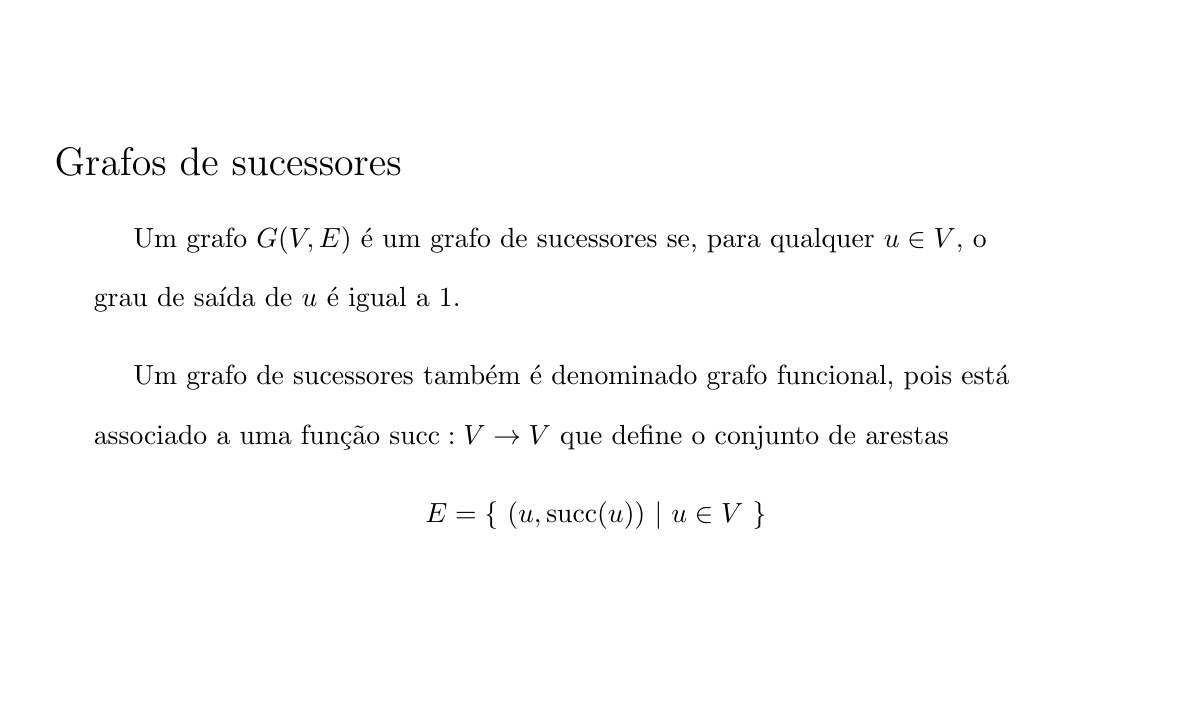
\begin{tikzpicture}
\node[draw,opacity=0] at (0, 0) {x};
\node[draw,opacity=0] at (14, 8) {x};

	\node[anchor=west] (title) at (0.0, 6.5) { \Large \bbbold{Grafos de sucessores} };

	\node[anchor=west] (a) at (1.0, 5.5) { \bbtext{Um grafo $G(V,E)$ é um \bbbold{grafo de sucessores} se, para qualquer $u\in V$, o} };

	\node[anchor=west] (a1) at (0.5, 4.75) { \bbtext{grau de saída de $u$ é igual a $1$.} };


	\node[anchor=west] (b) at (1.0, 3.75) { \bbtext{Um grafo de sucessores também é denominado \bbbold{grafo funcional}, pois está } };

	\node[anchor=west] (b1) at (0.5, 3.0) { \bbtext{associado a uma função $\mathrm{succ}: V \to V$ que define o conjunto de arestas} };

	\node[] (b2) at (7.0, 2.0) { $\displaystyle E = \{\ (u, \mathrm{succ}(u))\ |\ u\in V\ \}$ };

\end{tikzpicture}
\end{frame}
\begin{frame}[plain,t]
\begin{tikzpicture}
\node[draw,opacity=0] at (0, 0) {x};
\node[draw,opacity=0] at (14, 8) {x};

	\node[anchor=west] (title) at (0.0, 6.5) { \Large \bbbold{Características dos grafos de sucessores} };
\end{tikzpicture}
\end{frame}
\begin{frame}[plain,t]
\begin{tikzpicture}
\node[draw,opacity=0] at (0, 0) {x};
\node[draw,opacity=0] at (14, 8) {x};

	\node[anchor=west] (title) at (0.0, 6.5) { \Large \bbbold{Características dos grafos de sucessores} };

	\node[anchor=west] (a) at (1.0, 5.5) { $\star$ \bbtext{Um grafo de sucessores $G$ tem exatamente $|V|$ arestas} };

\end{tikzpicture}
\end{frame}
\begin{frame}[plain,t]
\begin{tikzpicture}
\node[draw,opacity=0] at (0, 0) {x};
\node[draw,opacity=0] at (14, 8) {x};

	\node[anchor=west] (title) at (0.0, 6.5) { \Large \bbbold{Características dos grafos de sucessores} };

	\node[anchor=west] (a) at (1.0, 5.5) { $\star$ \bbtext{Um grafo de sucessores $G$ tem exatamente $|V|$ arestas} };


	\node[anchor=west] (b) at (1.0, 4.5) { $\star$ \bbtext{Há, no mínimo, um ciclo em $G$} };

\end{tikzpicture}
\end{frame}
\begin{frame}[plain,t]

\begin{tikzpicture}
\node[draw,opacity=0] at (0, 0) {x};
\node[draw,opacity=0] at (14, 8) {x};

	\node[anchor=west] (title) at (0.0, 6.5) { \Large \bbbold{Características dos grafos de sucessores} };

	\node[anchor=west] (a) at (1.0, 5.5) { $\star$ \bbtext{Um grafo de sucessores $G$ tem exatamente $|V|$ arestas} };


	\node[anchor=west] (b) at (1.0, 4.5) { $\star$ \bbtext{Há, no mínimo, um ciclo em $G$} };


	\node[anchor=west] (c) at (1.0, 3.5) { $\star$ \bbtext{De fato, $G$ é composto por $k$ componentes, cada um deles com ao menos} };

	\node[anchor=west] (c1) at (0.5, 3.0) { \bbtext{um ciclo e um ou mais caminhos que levam a estes ciclos} };


\end{tikzpicture}
\end{frame}
\begin{frame}[plain,t]
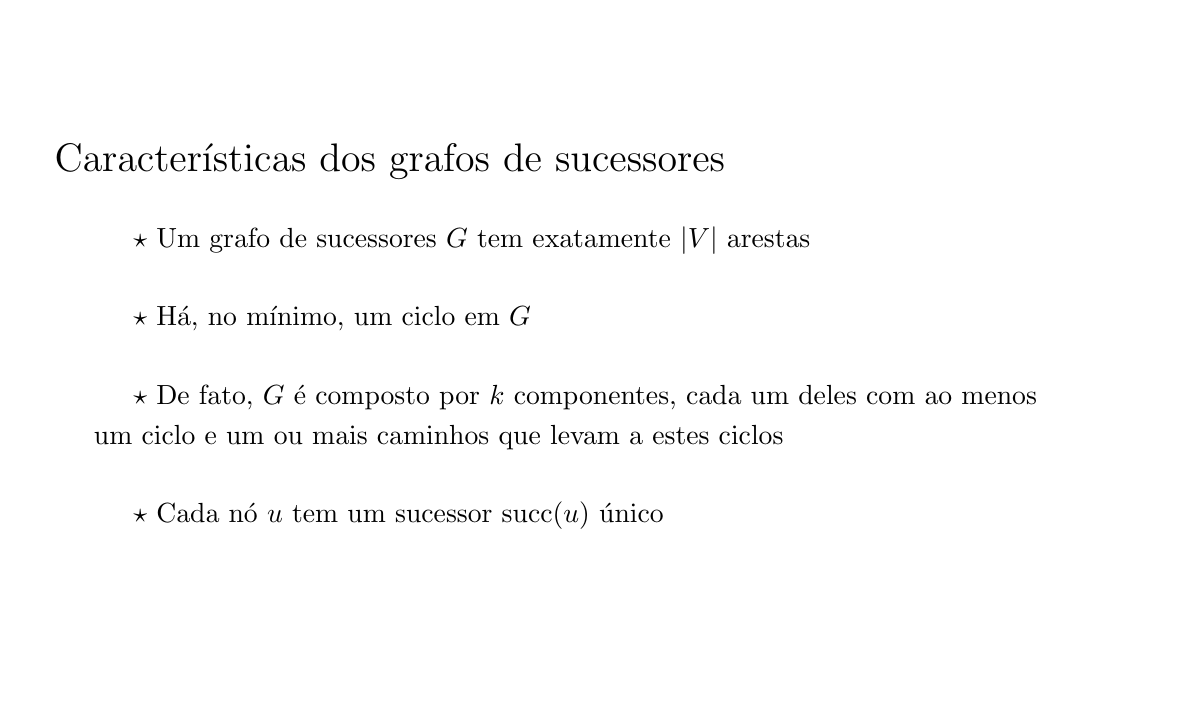
\begin{tikzpicture}
\node[draw,opacity=0] at (0, 0) {x};
\node[draw,opacity=0] at (14, 8) {x};

	\node[anchor=west] (title) at (0.0, 6.5) { \Large \bbbold{Características dos grafos de sucessores} };

	\node[anchor=west] (a) at (1.0, 5.5) { $\star$ \bbtext{Um grafo de sucessores $G$ tem exatamente $|V|$ arestas} };


	\node[anchor=west] (b) at (1.0, 4.5) { $\star$ \bbtext{Há, no mínimo, um ciclo em $G$} };


	\node[anchor=west] (c) at (1.0, 3.5) { $\star$ \bbtext{De fato, $G$ é composto por $k$ componentes, cada um deles com ao menos} };

	\node[anchor=west] (c1) at (0.5, 3.0) { \bbtext{um ciclo e um ou mais caminhos que levam a estes ciclos} };



	\node[anchor=west] (d) at (1.0, 2.0) { $\star$ \bbtext{Cada nó $u$ tem um sucessor $\mathrm{succ}(u)$ único} };

\end{tikzpicture}
\end{frame}
\begin{frame}[plain,t]
\begin{tikzpicture}
\node[draw,opacity=0] at (0, 0) {x};
\node[draw,opacity=0] at (14, 8) {x};

	\draw[thick] (2.0, 0.0) grid  (12.0, 1.0);

	\node[anchor=east] (succ) at (2.0, 0.5) { $\mathrm{succ}[u] = $ };

	\node[] (l1) at (2.5, 1.4) { \bbtext{1} };

	\node[] (l2) at (3.5, 1.4) { \bbtext{2} };

	\node[] (l3) at (4.5, 1.4) { \bbtext{3} };

	\node[] (l4) at (5.5, 1.4) { \bbtext{4} };

	\node[] (l5) at (6.5, 1.4) { \bbtext{5} };

	\node[] (l6) at (7.5, 1.4) { \bbtext{6} };

	\node[] (l7) at (8.5, 1.4) { \bbtext{7} };

	\node[] (l8) at (9.5, 1.4) { \bbtext{8} };

	\node[] (l9) at (10.5, 1.4) { \bbtext{9} };

	\node[] (l10) at (11.5, 1.4) { \bbtext{10} };

	\node[] (v1) at (2.5, 0.5) { $4$ };

	\node[] (v2) at (3.5, 0.5) { $5$ };

	\node[] (v3) at (4.5, 0.5) { $3$ };

	\node[] (v4) at (5.5, 0.5) { $7$ };

	\node[] (v5) at (6.5, 0.5) { $2$ };

	\node[] (v6) at (7.5, 0.5) { $8$ };

	\node[] (v7) at (8.5, 0.5) { $1$ };

	\node[] (v8) at (9.5, 0.5) { $9$ };

	\node[] (v9) at (10.5, 0.5) { $6$ };

	\node[] (v10) at (11.5, 0.5) { $8$ };

\end{tikzpicture}
\end{frame}
\begin{frame}[plain,t]
\begin{tikzpicture}
\node[draw,opacity=0] at (0, 0) {x};
\node[draw,opacity=0] at (14, 8) {x};

	\draw[thick] (2.0, 0.0) grid  (12.0, 1.0);

	\node[anchor=east] (succ) at (2.0, 0.5) { $\mathrm{succ}[u] = $ };

	\node[] (l1) at (2.5, 1.4) { \bbtext{1} };

	\node[] (l2) at (3.5, 1.4) { \bbtext{2} };

	\node[] (l3) at (4.5, 1.4) { \bbtext{3} };

	\node[] (l4) at (5.5, 1.4) { \bbtext{4} };

	\node[] (l5) at (6.5, 1.4) { \bbtext{5} };

	\node[] (l6) at (7.5, 1.4) { \bbtext{6} };

	\node[] (l7) at (8.5, 1.4) { \bbtext{7} };

	\node[] (l8) at (9.5, 1.4) { \bbtext{8} };

	\node[] (l9) at (10.5, 1.4) { \bbtext{9} };

	\node[] (l10) at (11.5, 1.4) { \bbtext{10} };

	\node[] (v1) at (2.5, 0.5) { $4$ };

	\node[] (v2) at (3.5, 0.5) { $5$ };

	\node[] (v3) at (4.5, 0.5) { $3$ };

	\node[] (v4) at (5.5, 0.5) { $7$ };

	\node[] (v5) at (6.5, 0.5) { $2$ };

	\node[] (v6) at (7.5, 0.5) { $8$ };

	\node[] (v7) at (8.5, 0.5) { $1$ };

	\node[] (v8) at (9.5, 0.5) { $9$ };

	\node[] (v9) at (10.5, 0.5) { $6$ };

	\node[] (v10) at (11.5, 0.5) { $8$ };


	\node[fill=BBCyan,very thick,draw,circle] (node1) at (1.0, 7.0) { \bbtext{1} };

\end{tikzpicture}
\end{frame}
\begin{frame}[plain,t]
\begin{tikzpicture}
\node[draw,opacity=0] at (0, 0) {x};
\node[draw,opacity=0] at (14, 8) {x};

	\draw[thick] (2.0, 0.0) grid  (12.0, 1.0);

	\node[anchor=east] (succ) at (2.0, 0.5) { $\mathrm{succ}[u] = $ };

	\node[] (l1) at (2.5, 1.4) { \bbtext{1} };

	\node[] (l2) at (3.5, 1.4) { \bbtext{2} };

	\node[] (l3) at (4.5, 1.4) { \bbtext{3} };

	\node[] (l4) at (5.5, 1.4) { \bbtext{4} };

	\node[] (l5) at (6.5, 1.4) { \bbtext{5} };

	\node[] (l6) at (7.5, 1.4) { \bbtext{6} };

	\node[] (l7) at (8.5, 1.4) { \bbtext{7} };

	\node[] (l8) at (9.5, 1.4) { \bbtext{8} };

	\node[] (l9) at (10.5, 1.4) { \bbtext{9} };

	\node[] (l10) at (11.5, 1.4) { \bbtext{10} };

	\node[] (v1) at (2.5, 0.5) { $4$ };

	\node[] (v2) at (3.5, 0.5) { $5$ };

	\node[] (v3) at (4.5, 0.5) { $3$ };

	\node[] (v4) at (5.5, 0.5) { $7$ };

	\node[] (v5) at (6.5, 0.5) { $2$ };

	\node[] (v6) at (7.5, 0.5) { $8$ };

	\node[] (v7) at (8.5, 0.5) { $1$ };

	\node[] (v8) at (9.5, 0.5) { $9$ };

	\node[] (v9) at (10.5, 0.5) { $6$ };

	\node[] (v10) at (11.5, 0.5) { $8$ };


	\node[fill=BBCyan,very thick,draw,circle] (node1) at (1.0, 7.0) { \bbtext{1} };

	\node[fill=BBCyan,very thick,draw,circle] (node4) at (3.0, 7.0) { \bbtext{4} };

	\draw[thick,-latex](node1) to (node4);

\end{tikzpicture}
\end{frame}
\begin{frame}[plain,t]
\begin{tikzpicture}
\node[draw,opacity=0] at (0, 0) {x};
\node[draw,opacity=0] at (14, 8) {x};

	\draw[thick] (2.0, 0.0) grid  (12.0, 1.0);

	\node[anchor=east] (succ) at (2.0, 0.5) { $\mathrm{succ}[u] = $ };

	\node[] (l1) at (2.5, 1.4) { \bbtext{1} };

	\node[] (l2) at (3.5, 1.4) { \bbtext{2} };

	\node[] (l3) at (4.5, 1.4) { \bbtext{3} };

	\node[] (l4) at (5.5, 1.4) { \bbtext{4} };

	\node[] (l5) at (6.5, 1.4) { \bbtext{5} };

	\node[] (l6) at (7.5, 1.4) { \bbtext{6} };

	\node[] (l7) at (8.5, 1.4) { \bbtext{7} };

	\node[] (l8) at (9.5, 1.4) { \bbtext{8} };

	\node[] (l9) at (10.5, 1.4) { \bbtext{9} };

	\node[] (l10) at (11.5, 1.4) { \bbtext{10} };

	\node[] (v1) at (2.5, 0.5) { $4$ };

	\node[] (v2) at (3.5, 0.5) { $5$ };

	\node[] (v3) at (4.5, 0.5) { $3$ };

	\node[] (v4) at (5.5, 0.5) { $7$ };

	\node[] (v5) at (6.5, 0.5) { $2$ };

	\node[] (v6) at (7.5, 0.5) { $8$ };

	\node[] (v7) at (8.5, 0.5) { $1$ };

	\node[] (v8) at (9.5, 0.5) { $9$ };

	\node[] (v9) at (10.5, 0.5) { $6$ };

	\node[] (v10) at (11.5, 0.5) { $8$ };


	\node[fill=BBCyan,very thick,draw,circle] (node1) at (1.0, 7.0) { \bbtext{1} };

	\node[fill=BBCyan,very thick,draw,circle] (node4) at (3.0, 7.0) { \bbtext{4} };

	\draw[thick,-latex](node1) to (node4);

	\node[fill=BBCyan,very thick,draw,circle] (node7) at (5.0, 7.0) { \bbtext{7} };

	\draw[thick,-latex](node4) to (node7);

\end{tikzpicture}
\end{frame}
\begin{frame}[plain,t]
\begin{tikzpicture}
\node[draw,opacity=0] at (0, 0) {x};
\node[draw,opacity=0] at (14, 8) {x};

	\draw[thick] (2.0, 0.0) grid  (12.0, 1.0);

	\node[anchor=east] (succ) at (2.0, 0.5) { $\mathrm{succ}[u] = $ };

	\node[] (l1) at (2.5, 1.4) { \bbtext{1} };

	\node[] (l2) at (3.5, 1.4) { \bbtext{2} };

	\node[] (l3) at (4.5, 1.4) { \bbtext{3} };

	\node[] (l4) at (5.5, 1.4) { \bbtext{4} };

	\node[] (l5) at (6.5, 1.4) { \bbtext{5} };

	\node[] (l6) at (7.5, 1.4) { \bbtext{6} };

	\node[] (l7) at (8.5, 1.4) { \bbtext{7} };

	\node[] (l8) at (9.5, 1.4) { \bbtext{8} };

	\node[] (l9) at (10.5, 1.4) { \bbtext{9} };

	\node[] (l10) at (11.5, 1.4) { \bbtext{10} };

	\node[] (v1) at (2.5, 0.5) { $4$ };

	\node[] (v2) at (3.5, 0.5) { $5$ };

	\node[] (v3) at (4.5, 0.5) { $3$ };

	\node[] (v4) at (5.5, 0.5) { $7$ };

	\node[] (v5) at (6.5, 0.5) { $2$ };

	\node[] (v6) at (7.5, 0.5) { $8$ };

	\node[] (v7) at (8.5, 0.5) { $1$ };

	\node[] (v8) at (9.5, 0.5) { $9$ };

	\node[] (v9) at (10.5, 0.5) { $6$ };

	\node[] (v10) at (11.5, 0.5) { $8$ };


	\node[fill=BBCyan,very thick,draw,circle] (node1) at (1.0, 7.0) { \bbtext{1} };

	\node[fill=BBCyan,very thick,draw,circle] (node4) at (3.0, 7.0) { \bbtext{4} };

	\draw[thick,-latex](node1) to (node4);

	\node[fill=BBCyan,very thick,draw,circle] (node7) at (5.0, 7.0) { \bbtext{7} };

	\draw[thick,-latex](node4) to (node7);

	\draw[thick,-latex](node7) to [bend left] (node1);

\end{tikzpicture}
\end{frame}
\begin{frame}[plain,t]
\begin{tikzpicture}
\node[draw,opacity=0] at (0, 0) {x};
\node[draw,opacity=0] at (14, 8) {x};

	\draw[thick] (2.0, 0.0) grid  (12.0, 1.0);

	\node[anchor=east] (succ) at (2.0, 0.5) { $\mathrm{succ}[u] = $ };

	\node[] (l1) at (2.5, 1.4) { \bbtext{1} };

	\node[] (l2) at (3.5, 1.4) { \bbtext{2} };

	\node[] (l3) at (4.5, 1.4) { \bbtext{3} };

	\node[] (l4) at (5.5, 1.4) { \bbtext{4} };

	\node[] (l5) at (6.5, 1.4) { \bbtext{5} };

	\node[] (l6) at (7.5, 1.4) { \bbtext{6} };

	\node[] (l7) at (8.5, 1.4) { \bbtext{7} };

	\node[] (l8) at (9.5, 1.4) { \bbtext{8} };

	\node[] (l9) at (10.5, 1.4) { \bbtext{9} };

	\node[] (l10) at (11.5, 1.4) { \bbtext{10} };

	\node[] (v1) at (2.5, 0.5) { $4$ };

	\node[] (v2) at (3.5, 0.5) { $5$ };

	\node[] (v3) at (4.5, 0.5) { $3$ };

	\node[] (v4) at (5.5, 0.5) { $7$ };

	\node[] (v5) at (6.5, 0.5) { $2$ };

	\node[] (v6) at (7.5, 0.5) { $8$ };

	\node[] (v7) at (8.5, 0.5) { $1$ };

	\node[] (v8) at (9.5, 0.5) { $9$ };

	\node[] (v9) at (10.5, 0.5) { $6$ };

	\node[] (v10) at (11.5, 0.5) { $8$ };


	\node[fill=BBCyan,very thick,draw,circle] (node1) at (1.0, 7.0) { \bbtext{1} };

	\node[fill=BBCyan,very thick,draw,circle] (node4) at (3.0, 7.0) { \bbtext{4} };

	\draw[thick,-latex](node1) to (node4);

	\node[fill=BBCyan,very thick,draw,circle] (node7) at (5.0, 7.0) { \bbtext{7} };

	\draw[thick,-latex](node4) to (node7);

	\draw[thick,-latex](node7) to [bend left] (node1);

	\node[fill=BBGreen,very thick,draw,circle] (node2) at (7.0, 7.0) { \bbtext{2} };

\end{tikzpicture}
\end{frame}
\begin{frame}[plain,t]
\begin{tikzpicture}
\node[draw,opacity=0] at (0, 0) {x};
\node[draw,opacity=0] at (14, 8) {x};

	\draw[thick] (2.0, 0.0) grid  (12.0, 1.0);

	\node[anchor=east] (succ) at (2.0, 0.5) { $\mathrm{succ}[u] = $ };

	\node[] (l1) at (2.5, 1.4) { \bbtext{1} };

	\node[] (l2) at (3.5, 1.4) { \bbtext{2} };

	\node[] (l3) at (4.5, 1.4) { \bbtext{3} };

	\node[] (l4) at (5.5, 1.4) { \bbtext{4} };

	\node[] (l5) at (6.5, 1.4) { \bbtext{5} };

	\node[] (l6) at (7.5, 1.4) { \bbtext{6} };

	\node[] (l7) at (8.5, 1.4) { \bbtext{7} };

	\node[] (l8) at (9.5, 1.4) { \bbtext{8} };

	\node[] (l9) at (10.5, 1.4) { \bbtext{9} };

	\node[] (l10) at (11.5, 1.4) { \bbtext{10} };

	\node[] (v1) at (2.5, 0.5) { $4$ };

	\node[] (v2) at (3.5, 0.5) { $5$ };

	\node[] (v3) at (4.5, 0.5) { $3$ };

	\node[] (v4) at (5.5, 0.5) { $7$ };

	\node[] (v5) at (6.5, 0.5) { $2$ };

	\node[] (v6) at (7.5, 0.5) { $8$ };

	\node[] (v7) at (8.5, 0.5) { $1$ };

	\node[] (v8) at (9.5, 0.5) { $9$ };

	\node[] (v9) at (10.5, 0.5) { $6$ };

	\node[] (v10) at (11.5, 0.5) { $8$ };


	\node[fill=BBCyan,very thick,draw,circle] (node1) at (1.0, 7.0) { \bbtext{1} };

	\node[fill=BBCyan,very thick,draw,circle] (node4) at (3.0, 7.0) { \bbtext{4} };

	\draw[thick,-latex](node1) to (node4);

	\node[fill=BBCyan,very thick,draw,circle] (node7) at (5.0, 7.0) { \bbtext{7} };

	\draw[thick,-latex](node4) to (node7);

	\draw[thick,-latex](node7) to [bend left] (node1);

	\node[fill=BBGreen,very thick,draw,circle] (node2) at (7.0, 7.0) { \bbtext{2} };

	\node[fill=BBGreen,very thick,draw,circle] (node5) at (7.0, 5.0) { \bbtext{5} };

	\draw[thick,-latex](node2) to (node5);

\end{tikzpicture}
\end{frame}
\begin{frame}[plain,t]
\begin{tikzpicture}
\node[draw,opacity=0] at (0, 0) {x};
\node[draw,opacity=0] at (14, 8) {x};

	\draw[thick] (2.0, 0.0) grid  (12.0, 1.0);

	\node[anchor=east] (succ) at (2.0, 0.5) { $\mathrm{succ}[u] = $ };

	\node[] (l1) at (2.5, 1.4) { \bbtext{1} };

	\node[] (l2) at (3.5, 1.4) { \bbtext{2} };

	\node[] (l3) at (4.5, 1.4) { \bbtext{3} };

	\node[] (l4) at (5.5, 1.4) { \bbtext{4} };

	\node[] (l5) at (6.5, 1.4) { \bbtext{5} };

	\node[] (l6) at (7.5, 1.4) { \bbtext{6} };

	\node[] (l7) at (8.5, 1.4) { \bbtext{7} };

	\node[] (l8) at (9.5, 1.4) { \bbtext{8} };

	\node[] (l9) at (10.5, 1.4) { \bbtext{9} };

	\node[] (l10) at (11.5, 1.4) { \bbtext{10} };

	\node[] (v1) at (2.5, 0.5) { $4$ };

	\node[] (v2) at (3.5, 0.5) { $5$ };

	\node[] (v3) at (4.5, 0.5) { $3$ };

	\node[] (v4) at (5.5, 0.5) { $7$ };

	\node[] (v5) at (6.5, 0.5) { $2$ };

	\node[] (v6) at (7.5, 0.5) { $8$ };

	\node[] (v7) at (8.5, 0.5) { $1$ };

	\node[] (v8) at (9.5, 0.5) { $9$ };

	\node[] (v9) at (10.5, 0.5) { $6$ };

	\node[] (v10) at (11.5, 0.5) { $8$ };


	\node[fill=BBCyan,very thick,draw,circle] (node1) at (1.0, 7.0) { \bbtext{1} };

	\node[fill=BBCyan,very thick,draw,circle] (node4) at (3.0, 7.0) { \bbtext{4} };

	\draw[thick,-latex](node1) to (node4);

	\node[fill=BBCyan,very thick,draw,circle] (node7) at (5.0, 7.0) { \bbtext{7} };

	\draw[thick,-latex](node4) to (node7);

	\draw[thick,-latex](node7) to [bend left] (node1);

	\node[fill=BBGreen,very thick,draw,circle] (node2) at (7.0, 7.0) { \bbtext{2} };

	\node[fill=BBGreen,very thick,draw,circle] (node5) at (7.0, 5.0) { \bbtext{5} };

	\draw[thick,-latex](node2) to (node5);

	\draw[thick,-latex](node5) to [bend left] (node2);

\end{tikzpicture}
\end{frame}
\begin{frame}[plain,t]
\begin{tikzpicture}
\node[draw,opacity=0] at (0, 0) {x};
\node[draw,opacity=0] at (14, 8) {x};

	\draw[thick] (2.0, 0.0) grid  (12.0, 1.0);

	\node[anchor=east] (succ) at (2.0, 0.5) { $\mathrm{succ}[u] = $ };

	\node[] (l1) at (2.5, 1.4) { \bbtext{1} };

	\node[] (l2) at (3.5, 1.4) { \bbtext{2} };

	\node[] (l3) at (4.5, 1.4) { \bbtext{3} };

	\node[] (l4) at (5.5, 1.4) { \bbtext{4} };

	\node[] (l5) at (6.5, 1.4) { \bbtext{5} };

	\node[] (l6) at (7.5, 1.4) { \bbtext{6} };

	\node[] (l7) at (8.5, 1.4) { \bbtext{7} };

	\node[] (l8) at (9.5, 1.4) { \bbtext{8} };

	\node[] (l9) at (10.5, 1.4) { \bbtext{9} };

	\node[] (l10) at (11.5, 1.4) { \bbtext{10} };

	\node[] (v1) at (2.5, 0.5) { $4$ };

	\node[] (v2) at (3.5, 0.5) { $5$ };

	\node[] (v3) at (4.5, 0.5) { $3$ };

	\node[] (v4) at (5.5, 0.5) { $7$ };

	\node[] (v5) at (6.5, 0.5) { $2$ };

	\node[] (v6) at (7.5, 0.5) { $8$ };

	\node[] (v7) at (8.5, 0.5) { $1$ };

	\node[] (v8) at (9.5, 0.5) { $9$ };

	\node[] (v9) at (10.5, 0.5) { $6$ };

	\node[] (v10) at (11.5, 0.5) { $8$ };


	\node[fill=BBCyan,very thick,draw,circle] (node1) at (1.0, 7.0) { \bbtext{1} };

	\node[fill=BBCyan,very thick,draw,circle] (node4) at (3.0, 7.0) { \bbtext{4} };

	\draw[thick,-latex](node1) to (node4);

	\node[fill=BBCyan,very thick,draw,circle] (node7) at (5.0, 7.0) { \bbtext{7} };

	\draw[thick,-latex](node4) to (node7);

	\draw[thick,-latex](node7) to [bend left] (node1);

	\node[fill=BBGreen,very thick,draw,circle] (node2) at (7.0, 7.0) { \bbtext{2} };

	\node[fill=BBGreen,very thick,draw,circle] (node5) at (7.0, 5.0) { \bbtext{5} };

	\draw[thick,-latex](node2) to (node5);

	\draw[thick,-latex](node5) to [bend left] (node2);


	\node[fill=BBOrange,very thick,draw,circle] (node3) at (7.0, 3.0) { \bbtext{3} };

\end{tikzpicture}
\end{frame}
\begin{frame}[plain,t]
\begin{tikzpicture}
\node[draw,opacity=0] at (0, 0) {x};
\node[draw,opacity=0] at (14, 8) {x};

	\draw[thick] (2.0, 0.0) grid  (12.0, 1.0);

	\node[anchor=east] (succ) at (2.0, 0.5) { $\mathrm{succ}[u] = $ };

	\node[] (l1) at (2.5, 1.4) { \bbtext{1} };

	\node[] (l2) at (3.5, 1.4) { \bbtext{2} };

	\node[] (l3) at (4.5, 1.4) { \bbtext{3} };

	\node[] (l4) at (5.5, 1.4) { \bbtext{4} };

	\node[] (l5) at (6.5, 1.4) { \bbtext{5} };

	\node[] (l6) at (7.5, 1.4) { \bbtext{6} };

	\node[] (l7) at (8.5, 1.4) { \bbtext{7} };

	\node[] (l8) at (9.5, 1.4) { \bbtext{8} };

	\node[] (l9) at (10.5, 1.4) { \bbtext{9} };

	\node[] (l10) at (11.5, 1.4) { \bbtext{10} };

	\node[] (v1) at (2.5, 0.5) { $4$ };

	\node[] (v2) at (3.5, 0.5) { $5$ };

	\node[] (v3) at (4.5, 0.5) { $3$ };

	\node[] (v4) at (5.5, 0.5) { $7$ };

	\node[] (v5) at (6.5, 0.5) { $2$ };

	\node[] (v6) at (7.5, 0.5) { $8$ };

	\node[] (v7) at (8.5, 0.5) { $1$ };

	\node[] (v8) at (9.5, 0.5) { $9$ };

	\node[] (v9) at (10.5, 0.5) { $6$ };

	\node[] (v10) at (11.5, 0.5) { $8$ };


	\node[fill=BBCyan,very thick,draw,circle] (node1) at (1.0, 7.0) { \bbtext{1} };

	\node[fill=BBCyan,very thick,draw,circle] (node4) at (3.0, 7.0) { \bbtext{4} };

	\draw[thick,-latex](node1) to (node4);

	\node[fill=BBCyan,very thick,draw,circle] (node7) at (5.0, 7.0) { \bbtext{7} };

	\draw[thick,-latex](node4) to (node7);

	\draw[thick,-latex](node7) to [bend left] (node1);

	\node[fill=BBGreen,very thick,draw,circle] (node2) at (7.0, 7.0) { \bbtext{2} };

	\node[fill=BBGreen,very thick,draw,circle] (node5) at (7.0, 5.0) { \bbtext{5} };

	\draw[thick,-latex](node2) to (node5);

	\draw[thick,-latex](node5) to [bend left] (node2);


	\node[fill=BBOrange,very thick,draw,circle] (node3) at (7.0, 3.0) { \bbtext{3} };

	\draw[thick,-latex](node3) to [loop left] (node3);

\end{tikzpicture}
\end{frame}
\begin{frame}[plain,t]
\begin{tikzpicture}
\node[draw,opacity=0] at (0, 0) {x};
\node[draw,opacity=0] at (14, 8) {x};

	\draw[thick] (2.0, 0.0) grid  (12.0, 1.0);

	\node[anchor=east] (succ) at (2.0, 0.5) { $\mathrm{succ}[u] = $ };

	\node[] (l1) at (2.5, 1.4) { \bbtext{1} };

	\node[] (l2) at (3.5, 1.4) { \bbtext{2} };

	\node[] (l3) at (4.5, 1.4) { \bbtext{3} };

	\node[] (l4) at (5.5, 1.4) { \bbtext{4} };

	\node[] (l5) at (6.5, 1.4) { \bbtext{5} };

	\node[] (l6) at (7.5, 1.4) { \bbtext{6} };

	\node[] (l7) at (8.5, 1.4) { \bbtext{7} };

	\node[] (l8) at (9.5, 1.4) { \bbtext{8} };

	\node[] (l9) at (10.5, 1.4) { \bbtext{9} };

	\node[] (l10) at (11.5, 1.4) { \bbtext{10} };

	\node[] (v1) at (2.5, 0.5) { $4$ };

	\node[] (v2) at (3.5, 0.5) { $5$ };

	\node[] (v3) at (4.5, 0.5) { $3$ };

	\node[] (v4) at (5.5, 0.5) { $7$ };

	\node[] (v5) at (6.5, 0.5) { $2$ };

	\node[] (v6) at (7.5, 0.5) { $8$ };

	\node[] (v7) at (8.5, 0.5) { $1$ };

	\node[] (v8) at (9.5, 0.5) { $9$ };

	\node[] (v9) at (10.5, 0.5) { $6$ };

	\node[] (v10) at (11.5, 0.5) { $8$ };


	\node[fill=BBCyan,very thick,draw,circle] (node1) at (1.0, 7.0) { \bbtext{1} };

	\node[fill=BBCyan,very thick,draw,circle] (node4) at (3.0, 7.0) { \bbtext{4} };

	\draw[thick,-latex](node1) to (node4);

	\node[fill=BBCyan,very thick,draw,circle] (node7) at (5.0, 7.0) { \bbtext{7} };

	\draw[thick,-latex](node4) to (node7);

	\draw[thick,-latex](node7) to [bend left] (node1);

	\node[fill=BBGreen,very thick,draw,circle] (node2) at (7.0, 7.0) { \bbtext{2} };

	\node[fill=BBGreen,very thick,draw,circle] (node5) at (7.0, 5.0) { \bbtext{5} };

	\draw[thick,-latex](node2) to (node5);

	\draw[thick,-latex](node5) to [bend left] (node2);


	\node[fill=BBOrange,very thick,draw,circle] (node3) at (7.0, 3.0) { \bbtext{3} };

	\draw[thick,-latex](node3) to [loop left] (node3);


	\node[fill=BBBlack,very thick,draw,circle] (node6) at (9.0, 7.0) { \bbchalk{6} };

\end{tikzpicture}
\end{frame}
\begin{frame}[plain,t]
\begin{tikzpicture}
\node[draw,opacity=0] at (0, 0) {x};
\node[draw,opacity=0] at (14, 8) {x};

	\draw[thick] (2.0, 0.0) grid  (12.0, 1.0);

	\node[anchor=east] (succ) at (2.0, 0.5) { $\mathrm{succ}[u] = $ };

	\node[] (l1) at (2.5, 1.4) { \bbtext{1} };

	\node[] (l2) at (3.5, 1.4) { \bbtext{2} };

	\node[] (l3) at (4.5, 1.4) { \bbtext{3} };

	\node[] (l4) at (5.5, 1.4) { \bbtext{4} };

	\node[] (l5) at (6.5, 1.4) { \bbtext{5} };

	\node[] (l6) at (7.5, 1.4) { \bbtext{6} };

	\node[] (l7) at (8.5, 1.4) { \bbtext{7} };

	\node[] (l8) at (9.5, 1.4) { \bbtext{8} };

	\node[] (l9) at (10.5, 1.4) { \bbtext{9} };

	\node[] (l10) at (11.5, 1.4) { \bbtext{10} };

	\node[] (v1) at (2.5, 0.5) { $4$ };

	\node[] (v2) at (3.5, 0.5) { $5$ };

	\node[] (v3) at (4.5, 0.5) { $3$ };

	\node[] (v4) at (5.5, 0.5) { $7$ };

	\node[] (v5) at (6.5, 0.5) { $2$ };

	\node[] (v6) at (7.5, 0.5) { $8$ };

	\node[] (v7) at (8.5, 0.5) { $1$ };

	\node[] (v8) at (9.5, 0.5) { $9$ };

	\node[] (v9) at (10.5, 0.5) { $6$ };

	\node[] (v10) at (11.5, 0.5) { $8$ };


	\node[fill=BBCyan,very thick,draw,circle] (node1) at (1.0, 7.0) { \bbtext{1} };

	\node[fill=BBCyan,very thick,draw,circle] (node4) at (3.0, 7.0) { \bbtext{4} };

	\draw[thick,-latex](node1) to (node4);

	\node[fill=BBCyan,very thick,draw,circle] (node7) at (5.0, 7.0) { \bbtext{7} };

	\draw[thick,-latex](node4) to (node7);

	\draw[thick,-latex](node7) to [bend left] (node1);

	\node[fill=BBGreen,very thick,draw,circle] (node2) at (7.0, 7.0) { \bbtext{2} };

	\node[fill=BBGreen,very thick,draw,circle] (node5) at (7.0, 5.0) { \bbtext{5} };

	\draw[thick,-latex](node2) to (node5);

	\draw[thick,-latex](node5) to [bend left] (node2);


	\node[fill=BBOrange,very thick,draw,circle] (node3) at (7.0, 3.0) { \bbtext{3} };

	\draw[thick,-latex](node3) to [loop left] (node3);


	\node[fill=BBBlack,very thick,draw,circle] (node6) at (9.0, 7.0) { \bbchalk{6} };


	\node[fill=BBBlack,very thick,draw,circle] (node8) at (11.0, 7.0) { \bbchalk{8} };

	\draw[thick,-latex](node6) to (node8);

\end{tikzpicture}
\end{frame}
\begin{frame}[plain,t]
\begin{tikzpicture}
\node[draw,opacity=0] at (0, 0) {x};
\node[draw,opacity=0] at (14, 8) {x};

	\draw[thick] (2.0, 0.0) grid  (12.0, 1.0);

	\node[anchor=east] (succ) at (2.0, 0.5) { $\mathrm{succ}[u] = $ };

	\node[] (l1) at (2.5, 1.4) { \bbtext{1} };

	\node[] (l2) at (3.5, 1.4) { \bbtext{2} };

	\node[] (l3) at (4.5, 1.4) { \bbtext{3} };

	\node[] (l4) at (5.5, 1.4) { \bbtext{4} };

	\node[] (l5) at (6.5, 1.4) { \bbtext{5} };

	\node[] (l6) at (7.5, 1.4) { \bbtext{6} };

	\node[] (l7) at (8.5, 1.4) { \bbtext{7} };

	\node[] (l8) at (9.5, 1.4) { \bbtext{8} };

	\node[] (l9) at (10.5, 1.4) { \bbtext{9} };

	\node[] (l10) at (11.5, 1.4) { \bbtext{10} };

	\node[] (v1) at (2.5, 0.5) { $4$ };

	\node[] (v2) at (3.5, 0.5) { $5$ };

	\node[] (v3) at (4.5, 0.5) { $3$ };

	\node[] (v4) at (5.5, 0.5) { $7$ };

	\node[] (v5) at (6.5, 0.5) { $2$ };

	\node[] (v6) at (7.5, 0.5) { $8$ };

	\node[] (v7) at (8.5, 0.5) { $1$ };

	\node[] (v8) at (9.5, 0.5) { $9$ };

	\node[] (v9) at (10.5, 0.5) { $6$ };

	\node[] (v10) at (11.5, 0.5) { $8$ };


	\node[fill=BBCyan,very thick,draw,circle] (node1) at (1.0, 7.0) { \bbtext{1} };

	\node[fill=BBCyan,very thick,draw,circle] (node4) at (3.0, 7.0) { \bbtext{4} };

	\draw[thick,-latex](node1) to (node4);

	\node[fill=BBCyan,very thick,draw,circle] (node7) at (5.0, 7.0) { \bbtext{7} };

	\draw[thick,-latex](node4) to (node7);

	\draw[thick,-latex](node7) to [bend left] (node1);

	\node[fill=BBGreen,very thick,draw,circle] (node2) at (7.0, 7.0) { \bbtext{2} };

	\node[fill=BBGreen,very thick,draw,circle] (node5) at (7.0, 5.0) { \bbtext{5} };

	\draw[thick,-latex](node2) to (node5);

	\draw[thick,-latex](node5) to [bend left] (node2);


	\node[fill=BBOrange,very thick,draw,circle] (node3) at (7.0, 3.0) { \bbtext{3} };

	\draw[thick,-latex](node3) to [loop left] (node3);


	\node[fill=BBBlack,very thick,draw,circle] (node6) at (9.0, 7.0) { \bbchalk{6} };


	\node[fill=BBBlack,very thick,draw,circle] (node8) at (11.0, 7.0) { \bbchalk{8} };

	\draw[thick,-latex](node6) to (node8);


	\node[fill=BBBlack,very thick,draw,circle] (node9) at (13.0, 7.0) { \bbchalk{9} };

	\draw[thick,-latex](node8) to (node9);
\end{tikzpicture}
\end{frame}
\begin{frame}[plain,t]
\begin{tikzpicture}
\node[draw,opacity=0] at (0, 0) {x};
\node[draw,opacity=0] at (14, 8) {x};

	\draw[thick] (2.0, 0.0) grid  (12.0, 1.0);

	\node[anchor=east] (succ) at (2.0, 0.5) { $\mathrm{succ}[u] = $ };

	\node[] (l1) at (2.5, 1.4) { \bbtext{1} };

	\node[] (l2) at (3.5, 1.4) { \bbtext{2} };

	\node[] (l3) at (4.5, 1.4) { \bbtext{3} };

	\node[] (l4) at (5.5, 1.4) { \bbtext{4} };

	\node[] (l5) at (6.5, 1.4) { \bbtext{5} };

	\node[] (l6) at (7.5, 1.4) { \bbtext{6} };

	\node[] (l7) at (8.5, 1.4) { \bbtext{7} };

	\node[] (l8) at (9.5, 1.4) { \bbtext{8} };

	\node[] (l9) at (10.5, 1.4) { \bbtext{9} };

	\node[] (l10) at (11.5, 1.4) { \bbtext{10} };

	\node[] (v1) at (2.5, 0.5) { $4$ };

	\node[] (v2) at (3.5, 0.5) { $5$ };

	\node[] (v3) at (4.5, 0.5) { $3$ };

	\node[] (v4) at (5.5, 0.5) { $7$ };

	\node[] (v5) at (6.5, 0.5) { $2$ };

	\node[] (v6) at (7.5, 0.5) { $8$ };

	\node[] (v7) at (8.5, 0.5) { $1$ };

	\node[] (v8) at (9.5, 0.5) { $9$ };

	\node[] (v9) at (10.5, 0.5) { $6$ };

	\node[] (v10) at (11.5, 0.5) { $8$ };


	\node[fill=BBCyan,very thick,draw,circle] (node1) at (1.0, 7.0) { \bbtext{1} };

	\node[fill=BBCyan,very thick,draw,circle] (node4) at (3.0, 7.0) { \bbtext{4} };

	\draw[thick,-latex](node1) to (node4);

	\node[fill=BBCyan,very thick,draw,circle] (node7) at (5.0, 7.0) { \bbtext{7} };

	\draw[thick,-latex](node4) to (node7);

	\draw[thick,-latex](node7) to [bend left] (node1);

	\node[fill=BBGreen,very thick,draw,circle] (node2) at (7.0, 7.0) { \bbtext{2} };

	\node[fill=BBGreen,very thick,draw,circle] (node5) at (7.0, 5.0) { \bbtext{5} };

	\draw[thick,-latex](node2) to (node5);

	\draw[thick,-latex](node5) to [bend left] (node2);


	\node[fill=BBOrange,very thick,draw,circle] (node3) at (7.0, 3.0) { \bbtext{3} };

	\draw[thick,-latex](node3) to [loop left] (node3);


	\node[fill=BBBlack,very thick,draw,circle] (node6) at (9.0, 7.0) { \bbchalk{6} };


	\node[fill=BBBlack,very thick,draw,circle] (node8) at (11.0, 7.0) { \bbchalk{8} };

	\draw[thick,-latex](node6) to (node8);


	\node[fill=BBBlack,very thick,draw,circle] (node9) at (13.0, 7.0) { \bbchalk{9} };

	\draw[thick,-latex](node8) to (node9);

	\draw[thick,-latex](node9) to [bend right] (node6);
\end{tikzpicture}
\end{frame}
\begin{frame}[plain,t]
\begin{tikzpicture}
\node[draw,opacity=0] at (0, 0) {x};
\node[draw,opacity=0] at (14, 8) {x};

	\draw[thick] (2.0, 0.0) grid  (12.0, 1.0);

	\node[anchor=east] (succ) at (2.0, 0.5) { $\mathrm{succ}[u] = $ };

	\node[] (l1) at (2.5, 1.4) { \bbtext{1} };

	\node[] (l2) at (3.5, 1.4) { \bbtext{2} };

	\node[] (l3) at (4.5, 1.4) { \bbtext{3} };

	\node[] (l4) at (5.5, 1.4) { \bbtext{4} };

	\node[] (l5) at (6.5, 1.4) { \bbtext{5} };

	\node[] (l6) at (7.5, 1.4) { \bbtext{6} };

	\node[] (l7) at (8.5, 1.4) { \bbtext{7} };

	\node[] (l8) at (9.5, 1.4) { \bbtext{8} };

	\node[] (l9) at (10.5, 1.4) { \bbtext{9} };

	\node[] (l10) at (11.5, 1.4) { \bbtext{10} };

	\node[] (v1) at (2.5, 0.5) { $4$ };

	\node[] (v2) at (3.5, 0.5) { $5$ };

	\node[] (v3) at (4.5, 0.5) { $3$ };

	\node[] (v4) at (5.5, 0.5) { $7$ };

	\node[] (v5) at (6.5, 0.5) { $2$ };

	\node[] (v6) at (7.5, 0.5) { $8$ };

	\node[] (v7) at (8.5, 0.5) { $1$ };

	\node[] (v8) at (9.5, 0.5) { $9$ };

	\node[] (v9) at (10.5, 0.5) { $6$ };

	\node[] (v10) at (11.5, 0.5) { $8$ };


	\node[fill=BBCyan,very thick,draw,circle] (node1) at (1.0, 7.0) { \bbtext{1} };

	\node[fill=BBCyan,very thick,draw,circle] (node4) at (3.0, 7.0) { \bbtext{4} };

	\draw[thick,-latex](node1) to (node4);

	\node[fill=BBCyan,very thick,draw,circle] (node7) at (5.0, 7.0) { \bbtext{7} };

	\draw[thick,-latex](node4) to (node7);

	\draw[thick,-latex](node7) to [bend left] (node1);

	\node[fill=BBGreen,very thick,draw,circle] (node2) at (7.0, 7.0) { \bbtext{2} };

	\node[fill=BBGreen,very thick,draw,circle] (node5) at (7.0, 5.0) { \bbtext{5} };

	\draw[thick,-latex](node2) to (node5);

	\draw[thick,-latex](node5) to [bend left] (node2);


	\node[fill=BBOrange,very thick,draw,circle] (node3) at (7.0, 3.0) { \bbtext{3} };

	\draw[thick,-latex](node3) to [loop left] (node3);


	\node[fill=BBBlack,very thick,draw,circle] (node6) at (9.0, 7.0) { \bbchalk{6} };


	\node[fill=BBBlack,very thick,draw,circle] (node8) at (11.0, 7.0) { \bbchalk{8} };

	\draw[thick,-latex](node6) to (node8);


	\node[fill=BBBlack,very thick,draw,circle] (node9) at (13.0, 7.0) { \bbchalk{9} };

	\draw[thick,-latex](node8) to (node9);

	\draw[thick,-latex](node9) to [bend right] (node6);

	\node[fill=BBBlack,very thick,draw,circle] (node10) at (11.0, 5.0) { \bbchalk{10} };

	\draw[thick,-latex](node10) to (node8);

\end{tikzpicture}
\end{frame}
\begin{frame}[plain,t]
\begin{tikzpicture}
\node[draw,opacity=0] at (0, 0) {x};
\node[draw,opacity=0] at (14, 8) {x};

	\node[anchor=west] (title) at (0.0, 6.0) { \Large \bbbold{$k$-ésimo sucessor} };
\end{tikzpicture}
\end{frame}
\begin{frame}[plain,t]
\begin{tikzpicture}
\node[draw,opacity=0] at (0, 0) {x};
\node[draw,opacity=0] at (14, 8) {x};

	\node[anchor=west] (title) at (0.0, 6.0) { \Large \bbbold{$k$-ésimo sucessor} };

	\node[anchor=west] (a) at (0.8, 5.0) { \bbtext{Seja $G$ um grafo de sucessores. O $k$\bbbold{-ésimo sucessor} de um vértice $u$ é definido} };

	\node[anchor=west] (a1) at (0.3, 4.25) { \bbtext{como} };

	\node[] (b) at (7.0, 3.25) { $\displaystyle \mathrm{succ}(u, k) = \mathrm{succ}^k(u) = \mathrm{succ}(\mathrm{succ}(\ldots \mathrm{succ}(u)))$ };

\end{tikzpicture}
\end{frame}
\begin{frame}[plain,t]
\begin{tikzpicture}
\node[draw,opacity=0] at (0, 0) {x};
\node[draw,opacity=0] at (14, 8) {x};

	\node[anchor=west] (title) at (0.0, 6.0) { \Large \bbbold{$k$-ésimo sucessor} };

	\node[anchor=west] (a) at (0.8, 5.0) { \bbtext{Seja $G$ um grafo de sucessores. O $k$\bbbold{-ésimo sucessor} de um vértice $u$ é definido} };

	\node[anchor=west] (a1) at (0.3, 4.25) { \bbtext{como} };

	\node[] (b) at (7.0, 3.25) { $\displaystyle \mathrm{succ}(u, k) = \mathrm{succ}^k(u) = \mathrm{succ}(\mathrm{succ}(\ldots \mathrm{succ}(u)))$ };

	\draw[color=BBViolet] (7.2, 2.95) -- (7.2, 2.8) -- node[below] { \footnotesize \bbcomment{$k$ vezes} } (10.7, 2.8) -- (10.7, 2.95);

\end{tikzpicture}
\end{frame}
\begin{frame}[plain,t]
\begin{tikzpicture}
\node[draw,opacity=0] at (0, 0) {x};
\node[draw,opacity=0] at (14, 8) {x};

	\node[anchor=west] (title) at (0.0, 6.5) { \Large \bbbold{Cálculo de $\mathrm{succ}(u, k)$ em $O(\log k)$} };
\end{tikzpicture}
\end{frame}
\begin{frame}[plain,t]
\begin{tikzpicture}
\node[draw,opacity=0] at (0, 0) {x};
\node[draw,opacity=0] at (14, 8) {x};

	\node[anchor=west] (title) at (0.0, 6.5) { \Large \bbbold{Cálculo de $\mathrm{succ}(u, k)$ em $O(\log k)$} };

	\node[anchor=west] (a) at (1.0, 5.5) { $\star$ \bbtext{A função $\mathrm{succ}(u, k)$ pode ser computada, trivialmente, em $O(k)$} };

\end{tikzpicture}
\end{frame}
\begin{frame}[plain,t]
\begin{tikzpicture}
\node[draw,opacity=0] at (0, 0) {x};
\node[draw,opacity=0] at (14, 8) {x};

	\node[anchor=west] (title) at (0.0, 6.5) { \Large \bbbold{Cálculo de $\mathrm{succ}(u, k)$ em $O(\log k)$} };

	\node[anchor=west] (a) at (1.0, 5.5) { $\star$ \bbtext{A função $\mathrm{succ}(u, k)$ pode ser computada, trivialmente, em $O(k)$} };


	\node[anchor=west] (b) at (1.0, 4.5) { $\star$ \bbtext{Contudo, é possível computar $\mathrm{succ}(u, v)$ em $O(\log k)$} };

\end{tikzpicture}
\end{frame}
\begin{frame}[plain,t]
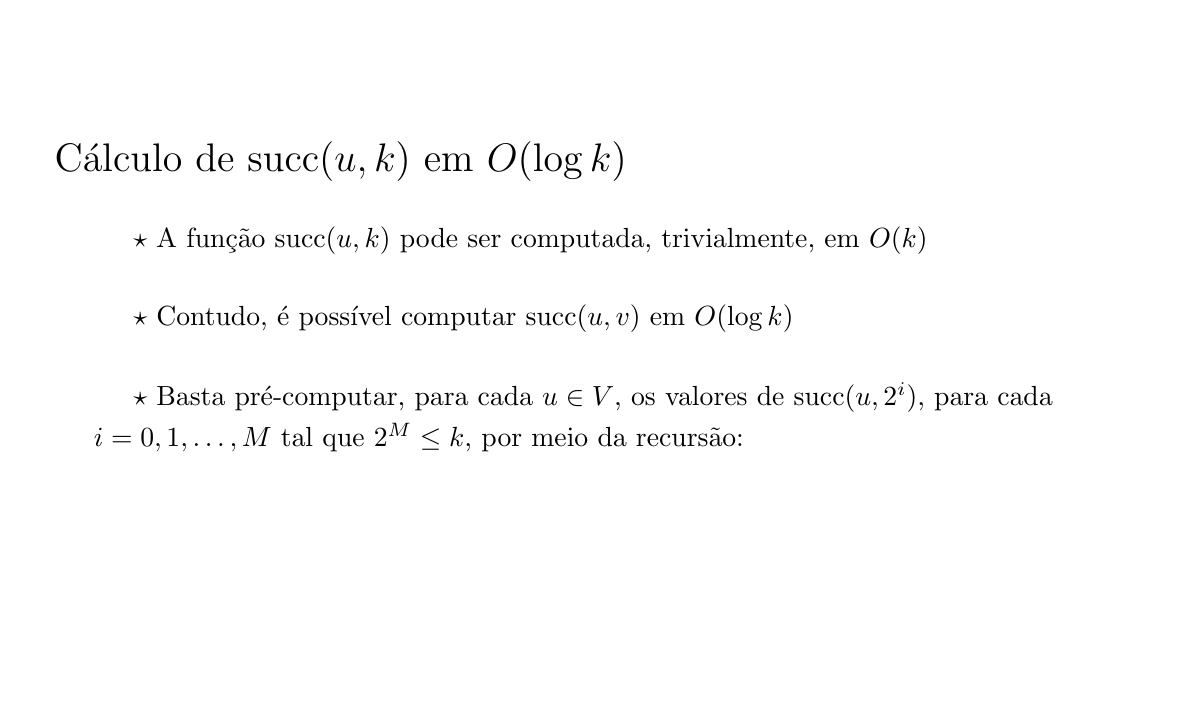
\begin{tikzpicture}
\node[draw,opacity=0] at (0, 0) {x};
\node[draw,opacity=0] at (14, 8) {x};

	\node[anchor=west] (title) at (0.0, 6.5) { \Large \bbbold{Cálculo de $\mathrm{succ}(u, k)$ em $O(\log k)$} };

	\node[anchor=west] (a) at (1.0, 5.5) { $\star$ \bbtext{A função $\mathrm{succ}(u, k)$ pode ser computada, trivialmente, em $O(k)$} };


	\node[anchor=west] (b) at (1.0, 4.5) { $\star$ \bbtext{Contudo, é possível computar $\mathrm{succ}(u, v)$ em $O(\log k)$} };


	\node[anchor=west] (c) at (1.0, 3.5) { $\star$ \bbtext{Basta pré-computar, para cada $u\in V$, os valores de $\mathrm{succ}(u, 2^i)$, para cada } };

	\node[anchor=west] (c1) at (0.5, 3.0) { \bbtext{$i = 0, 1, \ldots, M$ tal que $2^M\leq k$, por meio da recursão:} };


\end{tikzpicture}
\end{frame}
\begin{frame}[plain,t]
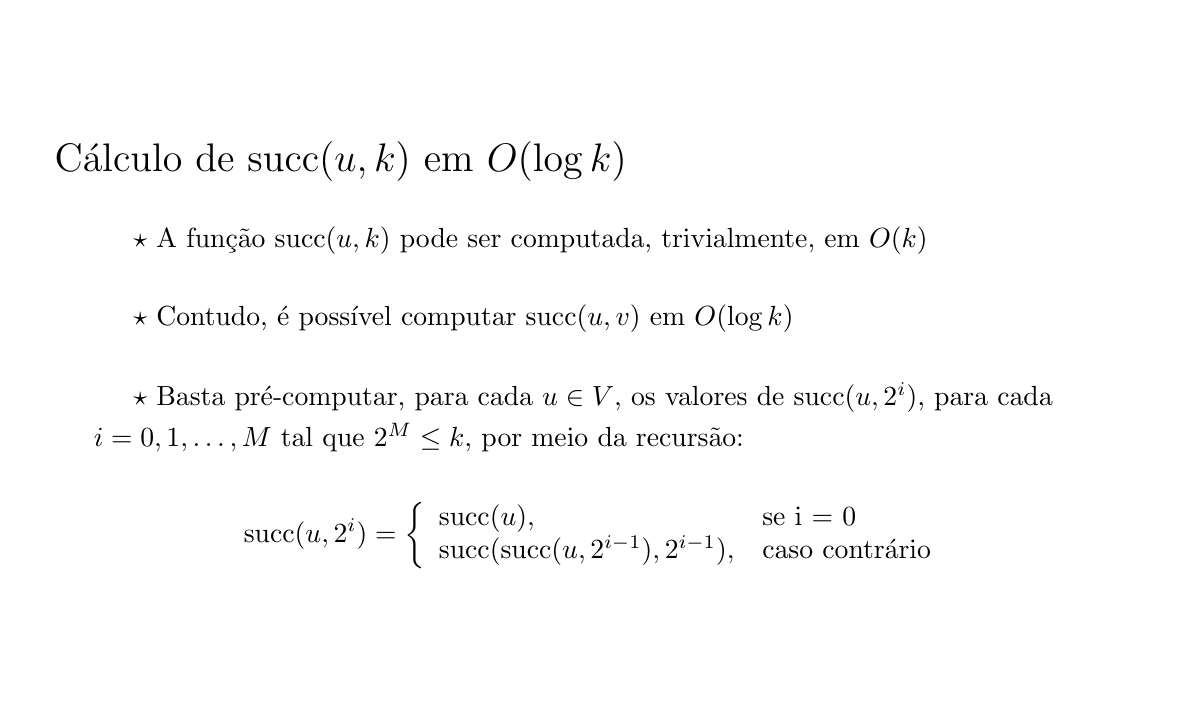
\begin{tikzpicture}
\node[draw,opacity=0] at (0, 0) {x};
\node[draw,opacity=0] at (14, 8) {x};

	\node[anchor=west] (title) at (0.0, 6.5) { \Large \bbbold{Cálculo de $\mathrm{succ}(u, k)$ em $O(\log k)$} };

	\node[anchor=west] (a) at (1.0, 5.5) { $\star$ \bbtext{A função $\mathrm{succ}(u, k)$ pode ser computada, trivialmente, em $O(k)$} };


	\node[anchor=west] (b) at (1.0, 4.5) { $\star$ \bbtext{Contudo, é possível computar $\mathrm{succ}(u, v)$ em $O(\log k)$} };


	\node[anchor=west] (c) at (1.0, 3.5) { $\star$ \bbtext{Basta pré-computar, para cada $u\in V$, os valores de $\mathrm{succ}(u, 2^i)$, para cada } };

	\node[anchor=west] (c1) at (0.5, 3.0) { \bbtext{$i = 0, 1, \ldots, M$ tal que $2^M\leq k$, por meio da recursão:} };



	\node[] (d) at (7.0, 1.75) { $\displaystyle \mathrm{succ}(u, 2^i) = \left\{ \begin{array}{ll} \mathrm{succ}(u), & \mbox{se}\ $i = 0$\\ \mathrm{succ}(\mathrm{succ}(u, 2^{i - 1}), 2^{i - 1}),& \mbox{caso contrário}\end{array}\right.$ };


\end{tikzpicture}
\end{frame}
\begin{frame}[plain,t]
\begin{tikzpicture}
\node[draw,opacity=0] at (0, 0) {x};
\node[draw,opacity=0] at (14, 8) {x};

	\node[anchor=west] (title) at (0.0, 6.5) { \Large \bbbold{Cálculo de $\mathrm{succ}(u, k)$ em $O(\log k)$} };

	\node[anchor=west] (a) at (1.0, 5.5) { $\star$ \bbtext{Estes valores podem ser pré-computados em $O(|V|\log k)$} };

\end{tikzpicture}
\end{frame}
\begin{frame}[plain,t]
\begin{tikzpicture}
\node[draw,opacity=0] at (0, 0) {x};
\node[draw,opacity=0] at (14, 8) {x};

	\node[anchor=west] (title) at (0.0, 6.5) { \Large \bbbold{Cálculo de $\mathrm{succ}(u, k)$ em $O(\log k)$} };

	\node[anchor=west] (a) at (1.0, 5.5) { $\star$ \bbtext{Estes valores podem ser pré-computados em $O(|V|\log k)$} };


	\node[anchor=west] (b) at (1.0, 4.5) { $\star$ \bbtext{De posse destes valores, $\mathrm{succ}(u, k)$ é dado por} };

	\node[] (c) at (7.0, 3.5) { $\displaystyle \mathrm{succ}(u, k) = \mathrm{succ}(\mathrm{succ}(\mathrm{succ}(\mathrm{succ}(u, 2^\alpha), 2^\beta), \ldots), 2^\omega),$ };

	\node[anchor=west] (d) at (0.5, 2.5) { \bbtext{onde $k = 2^\alpha 2^\beta \ldots 2^\omega$} };

\end{tikzpicture}
\end{frame}
\begin{frame}[plain,t]
\begin{tikzpicture}
\node[draw,opacity=0] at (0, 0) {x};
\node[draw,opacity=0] at (14, 8) {x};

	\node[very thick,draw,circle] (node1) at (7.0, 6.0) { \bbtext{1} };

	\node[very thick,draw,circle] (node2) at (8.5, 6.0) { \bbtext{2} };

	\node[very thick,draw,circle] (node3) at (10.0, 6.0) { \bbtext{3} };

	\node[very thick,draw,circle] (node4) at (10.0, 4.0) { \bbtext{4} };

	\node[very thick,draw,circle] (node5) at (11.5, 6.0) { \bbtext{5} };

	\node[very thick,draw,circle] (node6) at (13.0, 6.0) { \bbtext{6} };

	\draw[-latex,thick](node1) to (node2);

	\draw[-latex,thick](node2) to (node3);

	\draw[-latex,thick](node4) to (node3);

	\draw[-latex,thick](node3) to (node5);

	\draw[-latex,thick](node5) to (node6);

	\draw[-latex,thick](node6) to [bend right] (node1);

\end{tikzpicture}
\end{frame}
\begin{frame}[plain,t]
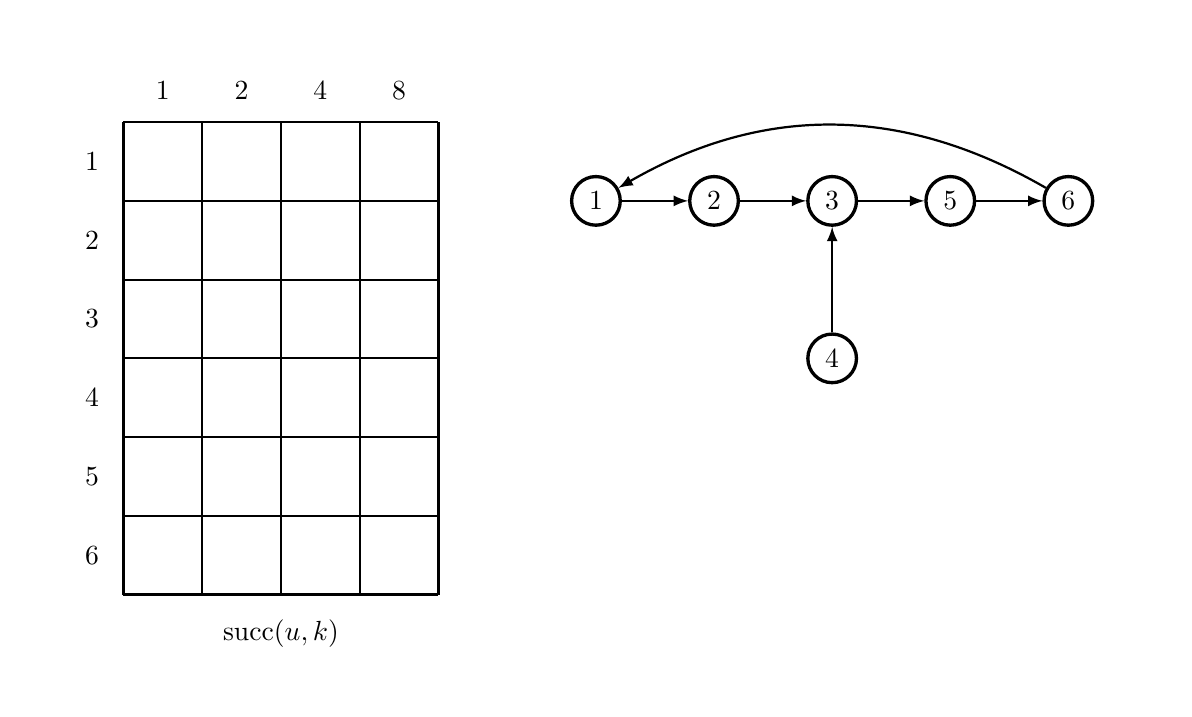
\begin{tikzpicture}
\node[draw,opacity=0] at (0, 0) {x};
\node[draw,opacity=0] at (14, 8) {x};

	\node[very thick,draw,circle] (node1) at (7.0, 6.0) { \bbtext{1} };

	\node[very thick,draw,circle] (node2) at (8.5, 6.0) { \bbtext{2} };

	\node[very thick,draw,circle] (node3) at (10.0, 6.0) { \bbtext{3} };

	\node[very thick,draw,circle] (node4) at (10.0, 4.0) { \bbtext{4} };

	\node[very thick,draw,circle] (node5) at (11.5, 6.0) { \bbtext{5} };

	\node[very thick,draw,circle] (node6) at (13.0, 6.0) { \bbtext{6} };

	\draw[-latex,thick](node1) to (node2);

	\draw[-latex,thick](node2) to (node3);

	\draw[-latex,thick](node4) to (node3);

	\draw[-latex,thick](node3) to (node5);

	\draw[-latex,thick](node5) to (node6);

	\draw[-latex,thick](node6) to [bend right] (node1);


	\draw[thick] (1.0, 1.0) grid  (5.0, 7.0);

	\node[] (k1) at (1.5, 7.4) { \bbtext{1} };

	\node[] (k2) at (2.5, 7.4) { \bbtext{2} };

	\node[] (k3) at (3.5, 7.4) { \bbtext{4} };

	\node[] (k4) at (4.5, 7.4) { \bbtext{8} };

	\node[] (x1) at (0.6, 6.5) { \bbtext{1} };

	\node[] (x2) at (0.6, 5.5) { \bbtext{2} };

	\node[] (x3) at (0.6, 4.5) { \bbtext{3} };

	\node[] (x4) at (0.6, 3.5) { \bbtext{4} };

	\node[] (x5) at (0.6, 2.5) { \bbtext{5} };

	\node[] (x6) at (0.6, 1.5) { \bbtext{6} };

	\node[] (succ) at (3.0, 0.5) { $\mathrm{succ}(u, k)$ };

\end{tikzpicture}
\end{frame}
\begin{frame}[plain,t]
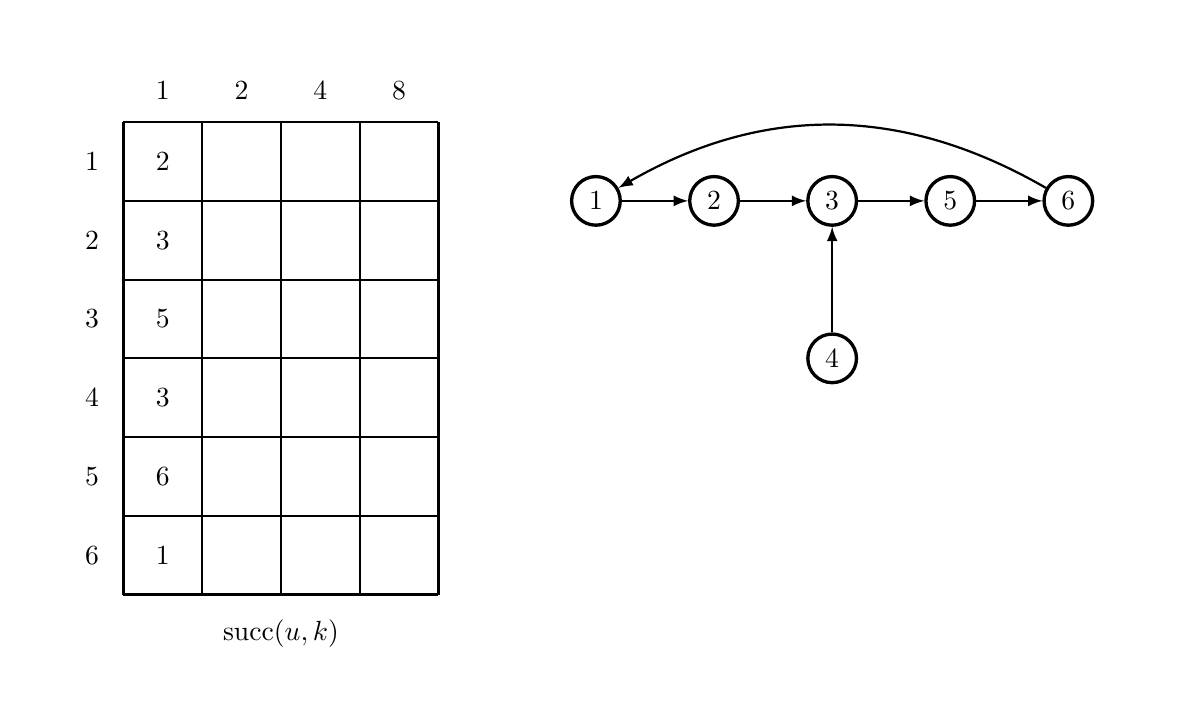
\begin{tikzpicture}
\node[draw,opacity=0] at (0, 0) {x};
\node[draw,opacity=0] at (14, 8) {x};

	\node[very thick,draw,circle] (node1) at (7.0, 6.0) { \bbtext{1} };

	\node[very thick,draw,circle] (node2) at (8.5, 6.0) { \bbtext{2} };

	\node[very thick,draw,circle] (node3) at (10.0, 6.0) { \bbtext{3} };

	\node[very thick,draw,circle] (node4) at (10.0, 4.0) { \bbtext{4} };

	\node[very thick,draw,circle] (node5) at (11.5, 6.0) { \bbtext{5} };

	\node[very thick,draw,circle] (node6) at (13.0, 6.0) { \bbtext{6} };

	\draw[-latex,thick](node1) to (node2);

	\draw[-latex,thick](node2) to (node3);

	\draw[-latex,thick](node4) to (node3);

	\draw[-latex,thick](node3) to (node5);

	\draw[-latex,thick](node5) to (node6);

	\draw[-latex,thick](node6) to [bend right] (node1);


	\draw[thick] (1.0, 1.0) grid  (5.0, 7.0);

	\node[] (k1) at (1.5, 7.4) { \bbtext{1} };

	\node[] (k2) at (2.5, 7.4) { \bbtext{2} };

	\node[] (k3) at (3.5, 7.4) { \bbtext{4} };

	\node[] (k4) at (4.5, 7.4) { \bbtext{8} };

	\node[] (x1) at (0.6, 6.5) { \bbtext{1} };

	\node[] (x2) at (0.6, 5.5) { \bbtext{2} };

	\node[] (x3) at (0.6, 4.5) { \bbtext{3} };

	\node[] (x4) at (0.6, 3.5) { \bbtext{4} };

	\node[] (x5) at (0.6, 2.5) { \bbtext{5} };

	\node[] (x6) at (0.6, 1.5) { \bbtext{6} };

	\node[] (succ) at (3.0, 0.5) { $\mathrm{succ}(u, k)$ };


	\node[] (v11) at (1.5, 6.5) { $2$ };

	\node[] (v21) at (1.5, 5.5) { $3$ };

	\node[] (v31) at (1.5, 4.5) { $5$ };

	\node[] (v41) at (1.5, 3.5) { $3$ };

	\node[] (v51) at (1.5, 2.5) { $6$ };

	\node[] (v61) at (1.5, 1.5) { $1$ };

\end{tikzpicture}
\end{frame}
\begin{frame}[plain,t]
\begin{tikzpicture}
\node[draw,opacity=0] at (0, 0) {x};
\node[draw,opacity=0] at (14, 8) {x};

	\node[very thick,draw,circle,fill=BBGreen] (node1) at (7.0, 6.0) { \bbtext{1} };

	\node[very thick,draw,circle] (node2) at (8.5, 6.0) { \bbtext{2} };

	\node[very thick,draw,circle] (node3) at (10.0, 6.0) { \bbtext{3} };

	\node[very thick,draw,circle] (node4) at (10.0, 4.0) { \bbtext{4} };

	\node[very thick,draw,circle] (node5) at (11.5, 6.0) { \bbtext{5} };

	\node[very thick,draw,circle] (node6) at (13.0, 6.0) { \bbtext{6} };

	\draw[-latex,thick](node1) to (node2);

	\draw[-latex,thick](node2) to (node3);

	\draw[-latex,thick](node4) to (node3);

	\draw[-latex,thick](node3) to (node5);

	\draw[-latex,thick](node5) to (node6);

	\draw[-latex,thick](node6) to [bend right] (node1);


	\draw[thick] (1.0, 1.0) grid  (5.0, 7.0);

	\node[] (k1) at (1.5, 7.4) { \bbtext{1} };

	\node[] (k2) at (2.5, 7.4) { \bbtext{2} };

	\node[] (k3) at (3.5, 7.4) { \bbtext{4} };

	\node[] (k4) at (4.5, 7.4) { \bbtext{8} };

	\node[] (x1) at (0.6, 6.5) { \bbtext{1} };

	\node[] (x2) at (0.6, 5.5) { \bbtext{2} };

	\node[] (x3) at (0.6, 4.5) { \bbtext{3} };

	\node[] (x4) at (0.6, 3.5) { \bbtext{4} };

	\node[] (x5) at (0.6, 2.5) { \bbtext{5} };

	\node[] (x6) at (0.6, 1.5) { \bbtext{6} };

	\node[] (succ) at (3.0, 0.5) { $\mathrm{succ}(u, k)$ };


	\node[] (v11) at (1.5, 6.5) { $2$ };

	\node[] (v21) at (1.5, 5.5) { $3$ };

	\node[] (v31) at (1.5, 4.5) { $5$ };

	\node[] (v41) at (1.5, 3.5) { $3$ };

	\node[] (v51) at (1.5, 2.5) { $6$ };

	\node[] (v61) at (1.5, 1.5) { $1$ };

\end{tikzpicture}
\end{frame}
\begin{frame}[plain,t]
\begin{tikzpicture}
\node[draw,opacity=0] at (0, 0) {x};
\node[draw,opacity=0] at (14, 8) {x};

	\node[very thick,draw,circle,fill=BBGreen] (node1) at (7.0, 6.0) { \bbtext{1} };

	\node[very thick,draw,circle,fill=BBOrange] (node2) at (8.5, 6.0) { \bbtext{2} };

	\node[very thick,draw,circle] (node3) at (10.0, 6.0) { \bbtext{3} };

	\node[very thick,draw,circle] (node4) at (10.0, 4.0) { \bbtext{4} };

	\node[very thick,draw,circle] (node5) at (11.5, 6.0) { \bbtext{5} };

	\node[very thick,draw,circle] (node6) at (13.0, 6.0) { \bbtext{6} };

	\draw[-latex,thick](node1) to (node2);

	\draw[-latex,thick](node2) to (node3);

	\draw[-latex,thick](node4) to (node3);

	\draw[-latex,thick](node3) to (node5);

	\draw[-latex,thick](node5) to (node6);

	\draw[-latex,thick](node6) to [bend right] (node1);


	\draw[thick] (1.0, 1.0) grid  (5.0, 7.0);

	\node[] (k1) at (1.5, 7.4) { \bbtext{1} };

	\node[] (k2) at (2.5, 7.4) { \bbtext{2} };

	\node[] (k3) at (3.5, 7.4) { \bbtext{4} };

	\node[] (k4) at (4.5, 7.4) { \bbtext{8} };

	\node[] (x1) at (0.6, 6.5) { \bbtext{1} };

	\node[] (x2) at (0.6, 5.5) { \bbtext{2} };

	\node[] (x3) at (0.6, 4.5) { \bbtext{3} };

	\node[] (x4) at (0.6, 3.5) { \bbtext{4} };

	\node[] (x5) at (0.6, 2.5) { \bbtext{5} };

	\node[] (x6) at (0.6, 1.5) { \bbtext{6} };

	\node[] (succ) at (3.0, 0.5) { $\mathrm{succ}(u, k)$ };


	\node[] (v11) at (1.5, 6.5) { $2$ };

	\node[] (v21) at (1.5, 5.5) { $3$ };

	\node[] (v31) at (1.5, 4.5) { $5$ };

	\node[] (v41) at (1.5, 3.5) { $3$ };

	\node[] (v51) at (1.5, 2.5) { $6$ };

	\node[] (v61) at (1.5, 1.5) { $1$ };

\end{tikzpicture}
\end{frame}
\begin{frame}[plain,t]
\begin{tikzpicture}
\node[draw,opacity=0] at (0, 0) {x};
\node[draw,opacity=0] at (14, 8) {x};

	\node[very thick,draw,circle,fill=BBGreen] (node1) at (7.0, 6.0) { \bbtext{1} };

	\node[very thick,draw,circle,fill=BBOrange] (node2) at (8.5, 6.0) { \bbtext{2} };

	\node[very thick,draw,circle,fill=BBCyan] (node3) at (10.0, 6.0) { \bbtext{3} };

	\node[very thick,draw,circle] (node4) at (10.0, 4.0) { \bbtext{4} };

	\node[very thick,draw,circle] (node5) at (11.5, 6.0) { \bbtext{5} };

	\node[very thick,draw,circle] (node6) at (13.0, 6.0) { \bbtext{6} };

	\draw[-latex,thick](node1) to (node2);

	\draw[-latex,thick](node2) to (node3);

	\draw[-latex,thick](node4) to (node3);

	\draw[-latex,thick](node3) to (node5);

	\draw[-latex,thick](node5) to (node6);

	\draw[-latex,thick](node6) to [bend right] (node1);


	\draw[thick] (1.0, 1.0) grid  (5.0, 7.0);

	\node[] (k1) at (1.5, 7.4) { \bbtext{1} };

	\node[] (k2) at (2.5, 7.4) { \bbtext{2} };

	\node[] (k3) at (3.5, 7.4) { \bbtext{4} };

	\node[] (k4) at (4.5, 7.4) { \bbtext{8} };

	\node[] (x1) at (0.6, 6.5) { \bbtext{1} };

	\node[] (x2) at (0.6, 5.5) { \bbtext{2} };

	\node[] (x3) at (0.6, 4.5) { \bbtext{3} };

	\node[] (x4) at (0.6, 3.5) { \bbtext{4} };

	\node[] (x5) at (0.6, 2.5) { \bbtext{5} };

	\node[] (x6) at (0.6, 1.5) { \bbtext{6} };

	\node[] (succ) at (3.0, 0.5) { $\mathrm{succ}(u, k)$ };


	\node[] (v11) at (1.5, 6.5) { $2$ };

	\node[] (v21) at (1.5, 5.5) { $3$ };

	\node[] (v31) at (1.5, 4.5) { $5$ };

	\node[] (v41) at (1.5, 3.5) { $3$ };

	\node[] (v51) at (1.5, 2.5) { $6$ };

	\node[] (v61) at (1.5, 1.5) { $1$ };

\end{tikzpicture}
\end{frame}
\begin{frame}[plain,t]
\begin{tikzpicture}
\node[draw,opacity=0] at (0, 0) {x};
\node[draw,opacity=0] at (14, 8) {x};

	\node[very thick,draw,circle,fill=BBGreen] (node1) at (7.0, 6.0) { \bbtext{1} };

	\node[very thick,draw,circle,fill=BBOrange] (node2) at (8.5, 6.0) { \bbtext{2} };

	\node[very thick,draw,circle,fill=BBCyan] (node3) at (10.0, 6.0) { \bbtext{3} };

	\node[very thick,draw,circle] (node4) at (10.0, 4.0) { \bbtext{4} };

	\node[very thick,draw,circle] (node5) at (11.5, 6.0) { \bbtext{5} };

	\node[very thick,draw,circle] (node6) at (13.0, 6.0) { \bbtext{6} };

	\draw[-latex,thick](node1) to (node2);

	\draw[-latex,thick](node2) to (node3);

	\draw[-latex,thick](node4) to (node3);

	\draw[-latex,thick](node3) to (node5);

	\draw[-latex,thick](node5) to (node6);

	\draw[-latex,thick](node6) to [bend right] (node1);


	\draw[thick] (1.0, 1.0) grid  (5.0, 7.0);

	\node[] (k1) at (1.5, 7.4) { \bbtext{1} };

	\node[] (k2) at (2.5, 7.4) { \bbtext{2} };

	\node[] (k3) at (3.5, 7.4) { \bbtext{4} };

	\node[] (k4) at (4.5, 7.4) { \bbtext{8} };

	\node[] (x1) at (0.6, 6.5) { \bbtext{1} };

	\node[] (x2) at (0.6, 5.5) { \bbtext{2} };

	\node[] (x3) at (0.6, 4.5) { \bbtext{3} };

	\node[] (x4) at (0.6, 3.5) { \bbtext{4} };

	\node[] (x5) at (0.6, 2.5) { \bbtext{5} };

	\node[] (x6) at (0.6, 1.5) { \bbtext{6} };

	\node[] (succ) at (3.0, 0.5) { $\mathrm{succ}(u, k)$ };


	\node[] (v11) at (1.5, 6.5) { $2$ };

	\node[] (v21) at (1.5, 5.5) { $3$ };

	\node[] (v31) at (1.5, 4.5) { $5$ };

	\node[] (v41) at (1.5, 3.5) { $3$ };

	\node[] (v51) at (1.5, 2.5) { $6$ };

	\node[] (v61) at (1.5, 1.5) { $1$ };

	\node[] (v12) at (2.5, 6.5) { $3$ };
\end{tikzpicture}
\end{frame}
\begin{frame}[plain,t]
\begin{tikzpicture}
\node[draw,opacity=0] at (0, 0) {x};
\node[draw,opacity=0] at (14, 8) {x};

	\node[very thick,draw,circle,fill=BBWhite] (node1) at (7.0, 6.0) { \bbtext{1} };

	\node[very thick,draw,circle,fill=BBGreen] (node2) at (8.5, 6.0) { \bbtext{2} };

	\node[very thick,draw,circle,fill=BBWhite] (node3) at (10.0, 6.0) { \bbtext{3} };

	\node[very thick,draw,circle] (node4) at (10.0, 4.0) { \bbtext{4} };

	\node[very thick,draw,circle] (node5) at (11.5, 6.0) { \bbtext{5} };

	\node[very thick,draw,circle] (node6) at (13.0, 6.0) { \bbtext{6} };

	\draw[-latex,thick](node1) to (node2);

	\draw[-latex,thick](node2) to (node3);

	\draw[-latex,thick](node4) to (node3);

	\draw[-latex,thick](node3) to (node5);

	\draw[-latex,thick](node5) to (node6);

	\draw[-latex,thick](node6) to [bend right] (node1);


	\draw[thick] (1.0, 1.0) grid  (5.0, 7.0);

	\node[] (k1) at (1.5, 7.4) { \bbtext{1} };

	\node[] (k2) at (2.5, 7.4) { \bbtext{2} };

	\node[] (k3) at (3.5, 7.4) { \bbtext{4} };

	\node[] (k4) at (4.5, 7.4) { \bbtext{8} };

	\node[] (x1) at (0.6, 6.5) { \bbtext{1} };

	\node[] (x2) at (0.6, 5.5) { \bbtext{2} };

	\node[] (x3) at (0.6, 4.5) { \bbtext{3} };

	\node[] (x4) at (0.6, 3.5) { \bbtext{4} };

	\node[] (x5) at (0.6, 2.5) { \bbtext{5} };

	\node[] (x6) at (0.6, 1.5) { \bbtext{6} };

	\node[] (succ) at (3.0, 0.5) { $\mathrm{succ}(u, k)$ };


	\node[] (v11) at (1.5, 6.5) { $2$ };

	\node[] (v21) at (1.5, 5.5) { $3$ };

	\node[] (v31) at (1.5, 4.5) { $5$ };

	\node[] (v41) at (1.5, 3.5) { $3$ };

	\node[] (v51) at (1.5, 2.5) { $6$ };

	\node[] (v61) at (1.5, 1.5) { $1$ };

	\node[] (v12) at (2.5, 6.5) { $3$ };

\end{tikzpicture}
\end{frame}
\begin{frame}[plain,t]
\begin{tikzpicture}
\node[draw,opacity=0] at (0, 0) {x};
\node[draw,opacity=0] at (14, 8) {x};

	\node[very thick,draw,circle,fill=BBWhite] (node1) at (7.0, 6.0) { \bbtext{1} };

	\node[very thick,draw,circle,fill=BBGreen] (node2) at (8.5, 6.0) { \bbtext{2} };

	\node[very thick,draw,circle,fill=BBOrange] (node3) at (10.0, 6.0) { \bbtext{3} };

	\node[very thick,draw,circle] (node4) at (10.0, 4.0) { \bbtext{4} };

	\node[very thick,draw,circle] (node5) at (11.5, 6.0) { \bbtext{5} };

	\node[very thick,draw,circle] (node6) at (13.0, 6.0) { \bbtext{6} };

	\draw[-latex,thick](node1) to (node2);

	\draw[-latex,thick](node2) to (node3);

	\draw[-latex,thick](node4) to (node3);

	\draw[-latex,thick](node3) to (node5);

	\draw[-latex,thick](node5) to (node6);

	\draw[-latex,thick](node6) to [bend right] (node1);


	\draw[thick] (1.0, 1.0) grid  (5.0, 7.0);

	\node[] (k1) at (1.5, 7.4) { \bbtext{1} };

	\node[] (k2) at (2.5, 7.4) { \bbtext{2} };

	\node[] (k3) at (3.5, 7.4) { \bbtext{4} };

	\node[] (k4) at (4.5, 7.4) { \bbtext{8} };

	\node[] (x1) at (0.6, 6.5) { \bbtext{1} };

	\node[] (x2) at (0.6, 5.5) { \bbtext{2} };

	\node[] (x3) at (0.6, 4.5) { \bbtext{3} };

	\node[] (x4) at (0.6, 3.5) { \bbtext{4} };

	\node[] (x5) at (0.6, 2.5) { \bbtext{5} };

	\node[] (x6) at (0.6, 1.5) { \bbtext{6} };

	\node[] (succ) at (3.0, 0.5) { $\mathrm{succ}(u, k)$ };


	\node[] (v11) at (1.5, 6.5) { $2$ };

	\node[] (v21) at (1.5, 5.5) { $3$ };

	\node[] (v31) at (1.5, 4.5) { $5$ };

	\node[] (v41) at (1.5, 3.5) { $3$ };

	\node[] (v51) at (1.5, 2.5) { $6$ };

	\node[] (v61) at (1.5, 1.5) { $1$ };

	\node[] (v12) at (2.5, 6.5) { $3$ };

\end{tikzpicture}
\end{frame}
\begin{frame}[plain,t]
\begin{tikzpicture}
\node[draw,opacity=0] at (0, 0) {x};
\node[draw,opacity=0] at (14, 8) {x};

	\node[very thick,draw,circle,fill=BBWhite] (node1) at (7.0, 6.0) { \bbtext{1} };

	\node[very thick,draw,circle,fill=BBGreen] (node2) at (8.5, 6.0) { \bbtext{2} };

	\node[very thick,draw,circle,fill=BBOrange] (node3) at (10.0, 6.0) { \bbtext{3} };

	\node[very thick,draw,circle] (node4) at (10.0, 4.0) { \bbtext{4} };

	\node[very thick,draw,circle,fill=BBCyan] (node5) at (11.5, 6.0) { \bbtext{5} };

	\node[very thick,draw,circle] (node6) at (13.0, 6.0) { \bbtext{6} };

	\draw[-latex,thick](node1) to (node2);

	\draw[-latex,thick](node2) to (node3);

	\draw[-latex,thick](node4) to (node3);

	\draw[-latex,thick](node3) to (node5);

	\draw[-latex,thick](node5) to (node6);

	\draw[-latex,thick](node6) to [bend right] (node1);


	\draw[thick] (1.0, 1.0) grid  (5.0, 7.0);

	\node[] (k1) at (1.5, 7.4) { \bbtext{1} };

	\node[] (k2) at (2.5, 7.4) { \bbtext{2} };

	\node[] (k3) at (3.5, 7.4) { \bbtext{4} };

	\node[] (k4) at (4.5, 7.4) { \bbtext{8} };

	\node[] (x1) at (0.6, 6.5) { \bbtext{1} };

	\node[] (x2) at (0.6, 5.5) { \bbtext{2} };

	\node[] (x3) at (0.6, 4.5) { \bbtext{3} };

	\node[] (x4) at (0.6, 3.5) { \bbtext{4} };

	\node[] (x5) at (0.6, 2.5) { \bbtext{5} };

	\node[] (x6) at (0.6, 1.5) { \bbtext{6} };

	\node[] (succ) at (3.0, 0.5) { $\mathrm{succ}(u, k)$ };


	\node[] (v11) at (1.5, 6.5) { $2$ };

	\node[] (v21) at (1.5, 5.5) { $3$ };

	\node[] (v31) at (1.5, 4.5) { $5$ };

	\node[] (v41) at (1.5, 3.5) { $3$ };

	\node[] (v51) at (1.5, 2.5) { $6$ };

	\node[] (v61) at (1.5, 1.5) { $1$ };

	\node[] (v12) at (2.5, 6.5) { $3$ };

\end{tikzpicture}
\end{frame}
\begin{frame}[plain,t]
\begin{tikzpicture}
\node[draw,opacity=0] at (0, 0) {x};
\node[draw,opacity=0] at (14, 8) {x};

	\node[very thick,draw,circle,fill=BBWhite] (node1) at (7.0, 6.0) { \bbtext{1} };

	\node[very thick,draw,circle,fill=BBGreen] (node2) at (8.5, 6.0) { \bbtext{2} };

	\node[very thick,draw,circle,fill=BBOrange] (node3) at (10.0, 6.0) { \bbtext{3} };

	\node[very thick,draw,circle] (node4) at (10.0, 4.0) { \bbtext{4} };

	\node[very thick,draw,circle,fill=BBCyan] (node5) at (11.5, 6.0) { \bbtext{5} };

	\node[very thick,draw,circle] (node6) at (13.0, 6.0) { \bbtext{6} };

	\draw[-latex,thick](node1) to (node2);

	\draw[-latex,thick](node2) to (node3);

	\draw[-latex,thick](node4) to (node3);

	\draw[-latex,thick](node3) to (node5);

	\draw[-latex,thick](node5) to (node6);

	\draw[-latex,thick](node6) to [bend right] (node1);


	\draw[thick] (1.0, 1.0) grid  (5.0, 7.0);

	\node[] (k1) at (1.5, 7.4) { \bbtext{1} };

	\node[] (k2) at (2.5, 7.4) { \bbtext{2} };

	\node[] (k3) at (3.5, 7.4) { \bbtext{4} };

	\node[] (k4) at (4.5, 7.4) { \bbtext{8} };

	\node[] (x1) at (0.6, 6.5) { \bbtext{1} };

	\node[] (x2) at (0.6, 5.5) { \bbtext{2} };

	\node[] (x3) at (0.6, 4.5) { \bbtext{3} };

	\node[] (x4) at (0.6, 3.5) { \bbtext{4} };

	\node[] (x5) at (0.6, 2.5) { \bbtext{5} };

	\node[] (x6) at (0.6, 1.5) { \bbtext{6} };

	\node[] (succ) at (3.0, 0.5) { $\mathrm{succ}(u, k)$ };


	\node[] (v11) at (1.5, 6.5) { $2$ };

	\node[] (v21) at (1.5, 5.5) { $3$ };

	\node[] (v31) at (1.5, 4.5) { $5$ };

	\node[] (v41) at (1.5, 3.5) { $3$ };

	\node[] (v51) at (1.5, 2.5) { $6$ };

	\node[] (v61) at (1.5, 1.5) { $1$ };

	\node[] (v12) at (2.5, 6.5) { $3$ };

	\node[] (v22) at (2.5, 5.5) { $5$ };
\end{tikzpicture}
\end{frame}
\begin{frame}[plain,t]
\begin{tikzpicture}
\node[draw,opacity=0] at (0, 0) {x};
\node[draw,opacity=0] at (14, 8) {x};

	\node[very thick,draw,circle,fill=BBWhite] (node1) at (7.0, 6.0) { \bbtext{1} };

	\node[very thick,draw,circle,fill=BBWhite] (node2) at (8.5, 6.0) { \bbtext{2} };

	\node[very thick,draw,circle,fill=BBGreen] (node3) at (10.0, 6.0) { \bbtext{3} };

	\node[very thick,draw,circle] (node4) at (10.0, 4.0) { \bbtext{4} };

	\node[very thick,draw,circle,fill=BBWhite] (node5) at (11.5, 6.0) { \bbtext{5} };

	\node[very thick,draw,circle] (node6) at (13.0, 6.0) { \bbtext{6} };

	\draw[-latex,thick](node1) to (node2);

	\draw[-latex,thick](node2) to (node3);

	\draw[-latex,thick](node4) to (node3);

	\draw[-latex,thick](node3) to (node5);

	\draw[-latex,thick](node5) to (node6);

	\draw[-latex,thick](node6) to [bend right] (node1);


	\draw[thick] (1.0, 1.0) grid  (5.0, 7.0);

	\node[] (k1) at (1.5, 7.4) { \bbtext{1} };

	\node[] (k2) at (2.5, 7.4) { \bbtext{2} };

	\node[] (k3) at (3.5, 7.4) { \bbtext{4} };

	\node[] (k4) at (4.5, 7.4) { \bbtext{8} };

	\node[] (x1) at (0.6, 6.5) { \bbtext{1} };

	\node[] (x2) at (0.6, 5.5) { \bbtext{2} };

	\node[] (x3) at (0.6, 4.5) { \bbtext{3} };

	\node[] (x4) at (0.6, 3.5) { \bbtext{4} };

	\node[] (x5) at (0.6, 2.5) { \bbtext{5} };

	\node[] (x6) at (0.6, 1.5) { \bbtext{6} };

	\node[] (succ) at (3.0, 0.5) { $\mathrm{succ}(u, k)$ };


	\node[] (v11) at (1.5, 6.5) { $2$ };

	\node[] (v21) at (1.5, 5.5) { $3$ };

	\node[] (v31) at (1.5, 4.5) { $5$ };

	\node[] (v41) at (1.5, 3.5) { $3$ };

	\node[] (v51) at (1.5, 2.5) { $6$ };

	\node[] (v61) at (1.5, 1.5) { $1$ };

	\node[] (v12) at (2.5, 6.5) { $3$ };

	\node[] (v22) at (2.5, 5.5) { $5$ };

\end{tikzpicture}
\end{frame}
\begin{frame}[plain,t]
\begin{tikzpicture}
\node[draw,opacity=0] at (0, 0) {x};
\node[draw,opacity=0] at (14, 8) {x};

	\node[very thick,draw,circle,fill=BBWhite] (node1) at (7.0, 6.0) { \bbtext{1} };

	\node[very thick,draw,circle,fill=BBWhite] (node2) at (8.5, 6.0) { \bbtext{2} };

	\node[very thick,draw,circle,fill=BBGreen] (node3) at (10.0, 6.0) { \bbtext{3} };

	\node[very thick,draw,circle] (node4) at (10.0, 4.0) { \bbtext{4} };

	\node[very thick,draw,circle,fill=BBOrange] (node5) at (11.5, 6.0) { \bbtext{5} };

	\node[very thick,draw,circle] (node6) at (13.0, 6.0) { \bbtext{6} };

	\draw[-latex,thick](node1) to (node2);

	\draw[-latex,thick](node2) to (node3);

	\draw[-latex,thick](node4) to (node3);

	\draw[-latex,thick](node3) to (node5);

	\draw[-latex,thick](node5) to (node6);

	\draw[-latex,thick](node6) to [bend right] (node1);


	\draw[thick] (1.0, 1.0) grid  (5.0, 7.0);

	\node[] (k1) at (1.5, 7.4) { \bbtext{1} };

	\node[] (k2) at (2.5, 7.4) { \bbtext{2} };

	\node[] (k3) at (3.5, 7.4) { \bbtext{4} };

	\node[] (k4) at (4.5, 7.4) { \bbtext{8} };

	\node[] (x1) at (0.6, 6.5) { \bbtext{1} };

	\node[] (x2) at (0.6, 5.5) { \bbtext{2} };

	\node[] (x3) at (0.6, 4.5) { \bbtext{3} };

	\node[] (x4) at (0.6, 3.5) { \bbtext{4} };

	\node[] (x5) at (0.6, 2.5) { \bbtext{5} };

	\node[] (x6) at (0.6, 1.5) { \bbtext{6} };

	\node[] (succ) at (3.0, 0.5) { $\mathrm{succ}(u, k)$ };


	\node[] (v11) at (1.5, 6.5) { $2$ };

	\node[] (v21) at (1.5, 5.5) { $3$ };

	\node[] (v31) at (1.5, 4.5) { $5$ };

	\node[] (v41) at (1.5, 3.5) { $3$ };

	\node[] (v51) at (1.5, 2.5) { $6$ };

	\node[] (v61) at (1.5, 1.5) { $1$ };

	\node[] (v12) at (2.5, 6.5) { $3$ };

	\node[] (v22) at (2.5, 5.5) { $5$ };

\end{tikzpicture}
\end{frame}
\begin{frame}[plain,t]
\begin{tikzpicture}
\node[draw,opacity=0] at (0, 0) {x};
\node[draw,opacity=0] at (14, 8) {x};

	\node[very thick,draw,circle,fill=BBWhite] (node1) at (7.0, 6.0) { \bbtext{1} };

	\node[very thick,draw,circle,fill=BBWhite] (node2) at (8.5, 6.0) { \bbtext{2} };

	\node[very thick,draw,circle,fill=BBGreen] (node3) at (10.0, 6.0) { \bbtext{3} };

	\node[very thick,draw,circle] (node4) at (10.0, 4.0) { \bbtext{4} };

	\node[very thick,draw,circle,fill=BBOrange] (node5) at (11.5, 6.0) { \bbtext{5} };

	\node[very thick,draw,circle,fill=BBCyan] (node6) at (13.0, 6.0) { \bbtext{6} };

	\draw[-latex,thick](node1) to (node2);

	\draw[-latex,thick](node2) to (node3);

	\draw[-latex,thick](node4) to (node3);

	\draw[-latex,thick](node3) to (node5);

	\draw[-latex,thick](node5) to (node6);

	\draw[-latex,thick](node6) to [bend right] (node1);


	\draw[thick] (1.0, 1.0) grid  (5.0, 7.0);

	\node[] (k1) at (1.5, 7.4) { \bbtext{1} };

	\node[] (k2) at (2.5, 7.4) { \bbtext{2} };

	\node[] (k3) at (3.5, 7.4) { \bbtext{4} };

	\node[] (k4) at (4.5, 7.4) { \bbtext{8} };

	\node[] (x1) at (0.6, 6.5) { \bbtext{1} };

	\node[] (x2) at (0.6, 5.5) { \bbtext{2} };

	\node[] (x3) at (0.6, 4.5) { \bbtext{3} };

	\node[] (x4) at (0.6, 3.5) { \bbtext{4} };

	\node[] (x5) at (0.6, 2.5) { \bbtext{5} };

	\node[] (x6) at (0.6, 1.5) { \bbtext{6} };

	\node[] (succ) at (3.0, 0.5) { $\mathrm{succ}(u, k)$ };


	\node[] (v11) at (1.5, 6.5) { $2$ };

	\node[] (v21) at (1.5, 5.5) { $3$ };

	\node[] (v31) at (1.5, 4.5) { $5$ };

	\node[] (v41) at (1.5, 3.5) { $3$ };

	\node[] (v51) at (1.5, 2.5) { $6$ };

	\node[] (v61) at (1.5, 1.5) { $1$ };

	\node[] (v12) at (2.5, 6.5) { $3$ };

	\node[] (v22) at (2.5, 5.5) { $5$ };

\end{tikzpicture}
\end{frame}
\begin{frame}[plain,t]
\begin{tikzpicture}
\node[draw,opacity=0] at (0, 0) {x};
\node[draw,opacity=0] at (14, 8) {x};

	\node[very thick,draw,circle,fill=BBWhite] (node1) at (7.0, 6.0) { \bbtext{1} };

	\node[very thick,draw,circle,fill=BBWhite] (node2) at (8.5, 6.0) { \bbtext{2} };

	\node[very thick,draw,circle,fill=BBGreen] (node3) at (10.0, 6.0) { \bbtext{3} };

	\node[very thick,draw,circle] (node4) at (10.0, 4.0) { \bbtext{4} };

	\node[very thick,draw,circle,fill=BBOrange] (node5) at (11.5, 6.0) { \bbtext{5} };

	\node[very thick,draw,circle,fill=BBCyan] (node6) at (13.0, 6.0) { \bbtext{6} };

	\draw[-latex,thick](node1) to (node2);

	\draw[-latex,thick](node2) to (node3);

	\draw[-latex,thick](node4) to (node3);

	\draw[-latex,thick](node3) to (node5);

	\draw[-latex,thick](node5) to (node6);

	\draw[-latex,thick](node6) to [bend right] (node1);


	\draw[thick] (1.0, 1.0) grid  (5.0, 7.0);

	\node[] (k1) at (1.5, 7.4) { \bbtext{1} };

	\node[] (k2) at (2.5, 7.4) { \bbtext{2} };

	\node[] (k3) at (3.5, 7.4) { \bbtext{4} };

	\node[] (k4) at (4.5, 7.4) { \bbtext{8} };

	\node[] (x1) at (0.6, 6.5) { \bbtext{1} };

	\node[] (x2) at (0.6, 5.5) { \bbtext{2} };

	\node[] (x3) at (0.6, 4.5) { \bbtext{3} };

	\node[] (x4) at (0.6, 3.5) { \bbtext{4} };

	\node[] (x5) at (0.6, 2.5) { \bbtext{5} };

	\node[] (x6) at (0.6, 1.5) { \bbtext{6} };

	\node[] (succ) at (3.0, 0.5) { $\mathrm{succ}(u, k)$ };


	\node[] (v11) at (1.5, 6.5) { $2$ };

	\node[] (v21) at (1.5, 5.5) { $3$ };

	\node[] (v31) at (1.5, 4.5) { $5$ };

	\node[] (v41) at (1.5, 3.5) { $3$ };

	\node[] (v51) at (1.5, 2.5) { $6$ };

	\node[] (v61) at (1.5, 1.5) { $1$ };

	\node[] (v12) at (2.5, 6.5) { $3$ };

	\node[] (v22) at (2.5, 5.5) { $5$ };

	\node[] (v32) at (2.5, 4.5) { $6$ };
\end{tikzpicture}
\end{frame}
\begin{frame}[plain,t]
\begin{tikzpicture}
\node[draw,opacity=0] at (0, 0) {x};
\node[draw,opacity=0] at (14, 8) {x};

	\node[very thick,draw,circle,fill=BBWhite] (node1) at (7.0, 6.0) { \bbtext{1} };

	\node[very thick,draw,circle,fill=BBWhite] (node2) at (8.5, 6.0) { \bbtext{2} };

	\node[very thick,draw,circle,fill=BBWhite] (node3) at (10.0, 6.0) { \bbtext{3} };

	\node[very thick,draw,circle,fill=BBGreen] (node4) at (10.0, 4.0) { \bbtext{4} };

	\node[very thick,draw,circle,fill=BBWhite] (node5) at (11.5, 6.0) { \bbtext{5} };

	\node[very thick,draw,circle,fill=BBWhite] (node6) at (13.0, 6.0) { \bbtext{6} };

	\draw[-latex,thick](node1) to (node2);

	\draw[-latex,thick](node2) to (node3);

	\draw[-latex,thick](node4) to (node3);

	\draw[-latex,thick](node3) to (node5);

	\draw[-latex,thick](node5) to (node6);

	\draw[-latex,thick](node6) to [bend right] (node1);


	\draw[thick] (1.0, 1.0) grid  (5.0, 7.0);

	\node[] (k1) at (1.5, 7.4) { \bbtext{1} };

	\node[] (k2) at (2.5, 7.4) { \bbtext{2} };

	\node[] (k3) at (3.5, 7.4) { \bbtext{4} };

	\node[] (k4) at (4.5, 7.4) { \bbtext{8} };

	\node[] (x1) at (0.6, 6.5) { \bbtext{1} };

	\node[] (x2) at (0.6, 5.5) { \bbtext{2} };

	\node[] (x3) at (0.6, 4.5) { \bbtext{3} };

	\node[] (x4) at (0.6, 3.5) { \bbtext{4} };

	\node[] (x5) at (0.6, 2.5) { \bbtext{5} };

	\node[] (x6) at (0.6, 1.5) { \bbtext{6} };

	\node[] (succ) at (3.0, 0.5) { $\mathrm{succ}(u, k)$ };


	\node[] (v11) at (1.5, 6.5) { $2$ };

	\node[] (v21) at (1.5, 5.5) { $3$ };

	\node[] (v31) at (1.5, 4.5) { $5$ };

	\node[] (v41) at (1.5, 3.5) { $3$ };

	\node[] (v51) at (1.5, 2.5) { $6$ };

	\node[] (v61) at (1.5, 1.5) { $1$ };

	\node[] (v12) at (2.5, 6.5) { $3$ };

	\node[] (v22) at (2.5, 5.5) { $5$ };

	\node[] (v32) at (2.5, 4.5) { $6$ };

\end{tikzpicture}
\end{frame}
\begin{frame}[plain,t]
\begin{tikzpicture}
\node[draw,opacity=0] at (0, 0) {x};
\node[draw,opacity=0] at (14, 8) {x};

	\node[very thick,draw,circle,fill=BBWhite] (node1) at (7.0, 6.0) { \bbtext{1} };

	\node[very thick,draw,circle,fill=BBWhite] (node2) at (8.5, 6.0) { \bbtext{2} };

	\node[very thick,draw,circle,fill=BBOrange] (node3) at (10.0, 6.0) { \bbtext{3} };

	\node[very thick,draw,circle,fill=BBGreen] (node4) at (10.0, 4.0) { \bbtext{4} };

	\node[very thick,draw,circle,fill=BBWhite] (node5) at (11.5, 6.0) { \bbtext{5} };

	\node[very thick,draw,circle,fill=BBWhite] (node6) at (13.0, 6.0) { \bbtext{6} };

	\draw[-latex,thick](node1) to (node2);

	\draw[-latex,thick](node2) to (node3);

	\draw[-latex,thick](node4) to (node3);

	\draw[-latex,thick](node3) to (node5);

	\draw[-latex,thick](node5) to (node6);

	\draw[-latex,thick](node6) to [bend right] (node1);


	\draw[thick] (1.0, 1.0) grid  (5.0, 7.0);

	\node[] (k1) at (1.5, 7.4) { \bbtext{1} };

	\node[] (k2) at (2.5, 7.4) { \bbtext{2} };

	\node[] (k3) at (3.5, 7.4) { \bbtext{4} };

	\node[] (k4) at (4.5, 7.4) { \bbtext{8} };

	\node[] (x1) at (0.6, 6.5) { \bbtext{1} };

	\node[] (x2) at (0.6, 5.5) { \bbtext{2} };

	\node[] (x3) at (0.6, 4.5) { \bbtext{3} };

	\node[] (x4) at (0.6, 3.5) { \bbtext{4} };

	\node[] (x5) at (0.6, 2.5) { \bbtext{5} };

	\node[] (x6) at (0.6, 1.5) { \bbtext{6} };

	\node[] (succ) at (3.0, 0.5) { $\mathrm{succ}(u, k)$ };


	\node[] (v11) at (1.5, 6.5) { $2$ };

	\node[] (v21) at (1.5, 5.5) { $3$ };

	\node[] (v31) at (1.5, 4.5) { $5$ };

	\node[] (v41) at (1.5, 3.5) { $3$ };

	\node[] (v51) at (1.5, 2.5) { $6$ };

	\node[] (v61) at (1.5, 1.5) { $1$ };

	\node[] (v12) at (2.5, 6.5) { $3$ };

	\node[] (v22) at (2.5, 5.5) { $5$ };

	\node[] (v32) at (2.5, 4.5) { $6$ };

\end{tikzpicture}
\end{frame}
\begin{frame}[plain,t]
\begin{tikzpicture}
\node[draw,opacity=0] at (0, 0) {x};
\node[draw,opacity=0] at (14, 8) {x};

	\node[very thick,draw,circle,fill=BBWhite] (node1) at (7.0, 6.0) { \bbtext{1} };

	\node[very thick,draw,circle,fill=BBWhite] (node2) at (8.5, 6.0) { \bbtext{2} };

	\node[very thick,draw,circle,fill=BBOrange] (node3) at (10.0, 6.0) { \bbtext{3} };

	\node[very thick,draw,circle,fill=BBGreen] (node4) at (10.0, 4.0) { \bbtext{4} };

	\node[very thick,draw,circle,fill=BBCyan] (node5) at (11.5, 6.0) { \bbtext{5} };

	\node[very thick,draw,circle,fill=BBWhite] (node6) at (13.0, 6.0) { \bbtext{6} };

	\draw[-latex,thick](node1) to (node2);

	\draw[-latex,thick](node2) to (node3);

	\draw[-latex,thick](node4) to (node3);

	\draw[-latex,thick](node3) to (node5);

	\draw[-latex,thick](node5) to (node6);

	\draw[-latex,thick](node6) to [bend right] (node1);


	\draw[thick] (1.0, 1.0) grid  (5.0, 7.0);

	\node[] (k1) at (1.5, 7.4) { \bbtext{1} };

	\node[] (k2) at (2.5, 7.4) { \bbtext{2} };

	\node[] (k3) at (3.5, 7.4) { \bbtext{4} };

	\node[] (k4) at (4.5, 7.4) { \bbtext{8} };

	\node[] (x1) at (0.6, 6.5) { \bbtext{1} };

	\node[] (x2) at (0.6, 5.5) { \bbtext{2} };

	\node[] (x3) at (0.6, 4.5) { \bbtext{3} };

	\node[] (x4) at (0.6, 3.5) { \bbtext{4} };

	\node[] (x5) at (0.6, 2.5) { \bbtext{5} };

	\node[] (x6) at (0.6, 1.5) { \bbtext{6} };

	\node[] (succ) at (3.0, 0.5) { $\mathrm{succ}(u, k)$ };


	\node[] (v11) at (1.5, 6.5) { $2$ };

	\node[] (v21) at (1.5, 5.5) { $3$ };

	\node[] (v31) at (1.5, 4.5) { $5$ };

	\node[] (v41) at (1.5, 3.5) { $3$ };

	\node[] (v51) at (1.5, 2.5) { $6$ };

	\node[] (v61) at (1.5, 1.5) { $1$ };

	\node[] (v12) at (2.5, 6.5) { $3$ };

	\node[] (v22) at (2.5, 5.5) { $5$ };

	\node[] (v32) at (2.5, 4.5) { $6$ };

\end{tikzpicture}
\end{frame}
\begin{frame}[plain,t]
\begin{tikzpicture}
\node[draw,opacity=0] at (0, 0) {x};
\node[draw,opacity=0] at (14, 8) {x};

	\node[very thick,draw,circle,fill=BBWhite] (node1) at (7.0, 6.0) { \bbtext{1} };

	\node[very thick,draw,circle,fill=BBWhite] (node2) at (8.5, 6.0) { \bbtext{2} };

	\node[very thick,draw,circle,fill=BBOrange] (node3) at (10.0, 6.0) { \bbtext{3} };

	\node[very thick,draw,circle,fill=BBGreen] (node4) at (10.0, 4.0) { \bbtext{4} };

	\node[very thick,draw,circle,fill=BBCyan] (node5) at (11.5, 6.0) { \bbtext{5} };

	\node[very thick,draw,circle,fill=BBWhite] (node6) at (13.0, 6.0) { \bbtext{6} };

	\draw[-latex,thick](node1) to (node2);

	\draw[-latex,thick](node2) to (node3);

	\draw[-latex,thick](node4) to (node3);

	\draw[-latex,thick](node3) to (node5);

	\draw[-latex,thick](node5) to (node6);

	\draw[-latex,thick](node6) to [bend right] (node1);


	\draw[thick] (1.0, 1.0) grid  (5.0, 7.0);

	\node[] (k1) at (1.5, 7.4) { \bbtext{1} };

	\node[] (k2) at (2.5, 7.4) { \bbtext{2} };

	\node[] (k3) at (3.5, 7.4) { \bbtext{4} };

	\node[] (k4) at (4.5, 7.4) { \bbtext{8} };

	\node[] (x1) at (0.6, 6.5) { \bbtext{1} };

	\node[] (x2) at (0.6, 5.5) { \bbtext{2} };

	\node[] (x3) at (0.6, 4.5) { \bbtext{3} };

	\node[] (x4) at (0.6, 3.5) { \bbtext{4} };

	\node[] (x5) at (0.6, 2.5) { \bbtext{5} };

	\node[] (x6) at (0.6, 1.5) { \bbtext{6} };

	\node[] (succ) at (3.0, 0.5) { $\mathrm{succ}(u, k)$ };


	\node[] (v11) at (1.5, 6.5) { $2$ };

	\node[] (v21) at (1.5, 5.5) { $3$ };

	\node[] (v31) at (1.5, 4.5) { $5$ };

	\node[] (v41) at (1.5, 3.5) { $3$ };

	\node[] (v51) at (1.5, 2.5) { $6$ };

	\node[] (v61) at (1.5, 1.5) { $1$ };

	\node[] (v12) at (2.5, 6.5) { $3$ };

	\node[] (v22) at (2.5, 5.5) { $5$ };

	\node[] (v32) at (2.5, 4.5) { $6$ };

	\node[] (v42) at (2.5, 3.5) { $5$ };
\end{tikzpicture}
\end{frame}
\begin{frame}[plain,t]
\begin{tikzpicture}
\node[draw,opacity=0] at (0, 0) {x};
\node[draw,opacity=0] at (14, 8) {x};

	\node[very thick,draw,circle,fill=BBWhite] (node1) at (7.0, 6.0) { \bbtext{1} };

	\node[very thick,draw,circle,fill=BBWhite] (node2) at (8.5, 6.0) { \bbtext{2} };

	\node[very thick,draw,circle,fill=BBWhite] (node3) at (10.0, 6.0) { \bbtext{3} };

	\node[very thick,draw,circle,fill=BBWhite] (node4) at (10.0, 4.0) { \bbtext{4} };

	\node[very thick,draw,circle,fill=BBGreen] (node5) at (11.5, 6.0) { \bbtext{5} };

	\node[very thick,draw,circle,fill=BBWhite] (node6) at (13.0, 6.0) { \bbtext{6} };

	\draw[-latex,thick](node1) to (node2);

	\draw[-latex,thick](node2) to (node3);

	\draw[-latex,thick](node4) to (node3);

	\draw[-latex,thick](node3) to (node5);

	\draw[-latex,thick](node5) to (node6);

	\draw[-latex,thick](node6) to [bend right] (node1);


	\draw[thick] (1.0, 1.0) grid  (5.0, 7.0);

	\node[] (k1) at (1.5, 7.4) { \bbtext{1} };

	\node[] (k2) at (2.5, 7.4) { \bbtext{2} };

	\node[] (k3) at (3.5, 7.4) { \bbtext{4} };

	\node[] (k4) at (4.5, 7.4) { \bbtext{8} };

	\node[] (x1) at (0.6, 6.5) { \bbtext{1} };

	\node[] (x2) at (0.6, 5.5) { \bbtext{2} };

	\node[] (x3) at (0.6, 4.5) { \bbtext{3} };

	\node[] (x4) at (0.6, 3.5) { \bbtext{4} };

	\node[] (x5) at (0.6, 2.5) { \bbtext{5} };

	\node[] (x6) at (0.6, 1.5) { \bbtext{6} };

	\node[] (succ) at (3.0, 0.5) { $\mathrm{succ}(u, k)$ };


	\node[] (v11) at (1.5, 6.5) { $2$ };

	\node[] (v21) at (1.5, 5.5) { $3$ };

	\node[] (v31) at (1.5, 4.5) { $5$ };

	\node[] (v41) at (1.5, 3.5) { $3$ };

	\node[] (v51) at (1.5, 2.5) { $6$ };

	\node[] (v61) at (1.5, 1.5) { $1$ };

	\node[] (v12) at (2.5, 6.5) { $3$ };

	\node[] (v22) at (2.5, 5.5) { $5$ };

	\node[] (v32) at (2.5, 4.5) { $6$ };

	\node[] (v42) at (2.5, 3.5) { $5$ };

\end{tikzpicture}
\end{frame}
\begin{frame}[plain,t]
\begin{tikzpicture}
\node[draw,opacity=0] at (0, 0) {x};
\node[draw,opacity=0] at (14, 8) {x};

	\node[very thick,draw,circle,fill=BBWhite] (node1) at (7.0, 6.0) { \bbtext{1} };

	\node[very thick,draw,circle,fill=BBWhite] (node2) at (8.5, 6.0) { \bbtext{2} };

	\node[very thick,draw,circle,fill=BBWhite] (node3) at (10.0, 6.0) { \bbtext{3} };

	\node[very thick,draw,circle,fill=BBWhite] (node4) at (10.0, 4.0) { \bbtext{4} };

	\node[very thick,draw,circle,fill=BBGreen] (node5) at (11.5, 6.0) { \bbtext{5} };

	\node[very thick,draw,circle,fill=BBOrange] (node6) at (13.0, 6.0) { \bbtext{6} };

	\draw[-latex,thick](node1) to (node2);

	\draw[-latex,thick](node2) to (node3);

	\draw[-latex,thick](node4) to (node3);

	\draw[-latex,thick](node3) to (node5);

	\draw[-latex,thick](node5) to (node6);

	\draw[-latex,thick](node6) to [bend right] (node1);


	\draw[thick] (1.0, 1.0) grid  (5.0, 7.0);

	\node[] (k1) at (1.5, 7.4) { \bbtext{1} };

	\node[] (k2) at (2.5, 7.4) { \bbtext{2} };

	\node[] (k3) at (3.5, 7.4) { \bbtext{4} };

	\node[] (k4) at (4.5, 7.4) { \bbtext{8} };

	\node[] (x1) at (0.6, 6.5) { \bbtext{1} };

	\node[] (x2) at (0.6, 5.5) { \bbtext{2} };

	\node[] (x3) at (0.6, 4.5) { \bbtext{3} };

	\node[] (x4) at (0.6, 3.5) { \bbtext{4} };

	\node[] (x5) at (0.6, 2.5) { \bbtext{5} };

	\node[] (x6) at (0.6, 1.5) { \bbtext{6} };

	\node[] (succ) at (3.0, 0.5) { $\mathrm{succ}(u, k)$ };


	\node[] (v11) at (1.5, 6.5) { $2$ };

	\node[] (v21) at (1.5, 5.5) { $3$ };

	\node[] (v31) at (1.5, 4.5) { $5$ };

	\node[] (v41) at (1.5, 3.5) { $3$ };

	\node[] (v51) at (1.5, 2.5) { $6$ };

	\node[] (v61) at (1.5, 1.5) { $1$ };

	\node[] (v12) at (2.5, 6.5) { $3$ };

	\node[] (v22) at (2.5, 5.5) { $5$ };

	\node[] (v32) at (2.5, 4.5) { $6$ };

	\node[] (v42) at (2.5, 3.5) { $5$ };

\end{tikzpicture}
\end{frame}
\begin{frame}[plain,t]
\begin{tikzpicture}
\node[draw,opacity=0] at (0, 0) {x};
\node[draw,opacity=0] at (14, 8) {x};

	\node[very thick,draw,circle,fill=BBCyan] (node1) at (7.0, 6.0) { \bbtext{1} };

	\node[very thick,draw,circle,fill=BBWhite] (node2) at (8.5, 6.0) { \bbtext{2} };

	\node[very thick,draw,circle,fill=BBWhite] (node3) at (10.0, 6.0) { \bbtext{3} };

	\node[very thick,draw,circle,fill=BBWhite] (node4) at (10.0, 4.0) { \bbtext{4} };

	\node[very thick,draw,circle,fill=BBGreen] (node5) at (11.5, 6.0) { \bbtext{5} };

	\node[very thick,draw,circle,fill=BBOrange] (node6) at (13.0, 6.0) { \bbtext{6} };

	\draw[-latex,thick](node1) to (node2);

	\draw[-latex,thick](node2) to (node3);

	\draw[-latex,thick](node4) to (node3);

	\draw[-latex,thick](node3) to (node5);

	\draw[-latex,thick](node5) to (node6);

	\draw[-latex,thick](node6) to [bend right] (node1);


	\draw[thick] (1.0, 1.0) grid  (5.0, 7.0);

	\node[] (k1) at (1.5, 7.4) { \bbtext{1} };

	\node[] (k2) at (2.5, 7.4) { \bbtext{2} };

	\node[] (k3) at (3.5, 7.4) { \bbtext{4} };

	\node[] (k4) at (4.5, 7.4) { \bbtext{8} };

	\node[] (x1) at (0.6, 6.5) { \bbtext{1} };

	\node[] (x2) at (0.6, 5.5) { \bbtext{2} };

	\node[] (x3) at (0.6, 4.5) { \bbtext{3} };

	\node[] (x4) at (0.6, 3.5) { \bbtext{4} };

	\node[] (x5) at (0.6, 2.5) { \bbtext{5} };

	\node[] (x6) at (0.6, 1.5) { \bbtext{6} };

	\node[] (succ) at (3.0, 0.5) { $\mathrm{succ}(u, k)$ };


	\node[] (v11) at (1.5, 6.5) { $2$ };

	\node[] (v21) at (1.5, 5.5) { $3$ };

	\node[] (v31) at (1.5, 4.5) { $5$ };

	\node[] (v41) at (1.5, 3.5) { $3$ };

	\node[] (v51) at (1.5, 2.5) { $6$ };

	\node[] (v61) at (1.5, 1.5) { $1$ };

	\node[] (v12) at (2.5, 6.5) { $3$ };

	\node[] (v22) at (2.5, 5.5) { $5$ };

	\node[] (v32) at (2.5, 4.5) { $6$ };

	\node[] (v42) at (2.5, 3.5) { $5$ };

\end{tikzpicture}
\end{frame}
\begin{frame}[plain,t]
\begin{tikzpicture}
\node[draw,opacity=0] at (0, 0) {x};
\node[draw,opacity=0] at (14, 8) {x};

	\node[very thick,draw,circle,fill=BBCyan] (node1) at (7.0, 6.0) { \bbtext{1} };

	\node[very thick,draw,circle,fill=BBWhite] (node2) at (8.5, 6.0) { \bbtext{2} };

	\node[very thick,draw,circle,fill=BBWhite] (node3) at (10.0, 6.0) { \bbtext{3} };

	\node[very thick,draw,circle,fill=BBWhite] (node4) at (10.0, 4.0) { \bbtext{4} };

	\node[very thick,draw,circle,fill=BBGreen] (node5) at (11.5, 6.0) { \bbtext{5} };

	\node[very thick,draw,circle,fill=BBOrange] (node6) at (13.0, 6.0) { \bbtext{6} };

	\draw[-latex,thick](node1) to (node2);

	\draw[-latex,thick](node2) to (node3);

	\draw[-latex,thick](node4) to (node3);

	\draw[-latex,thick](node3) to (node5);

	\draw[-latex,thick](node5) to (node6);

	\draw[-latex,thick](node6) to [bend right] (node1);


	\draw[thick] (1.0, 1.0) grid  (5.0, 7.0);

	\node[] (k1) at (1.5, 7.4) { \bbtext{1} };

	\node[] (k2) at (2.5, 7.4) { \bbtext{2} };

	\node[] (k3) at (3.5, 7.4) { \bbtext{4} };

	\node[] (k4) at (4.5, 7.4) { \bbtext{8} };

	\node[] (x1) at (0.6, 6.5) { \bbtext{1} };

	\node[] (x2) at (0.6, 5.5) { \bbtext{2} };

	\node[] (x3) at (0.6, 4.5) { \bbtext{3} };

	\node[] (x4) at (0.6, 3.5) { \bbtext{4} };

	\node[] (x5) at (0.6, 2.5) { \bbtext{5} };

	\node[] (x6) at (0.6, 1.5) { \bbtext{6} };

	\node[] (succ) at (3.0, 0.5) { $\mathrm{succ}(u, k)$ };


	\node[] (v11) at (1.5, 6.5) { $2$ };

	\node[] (v21) at (1.5, 5.5) { $3$ };

	\node[] (v31) at (1.5, 4.5) { $5$ };

	\node[] (v41) at (1.5, 3.5) { $3$ };

	\node[] (v51) at (1.5, 2.5) { $6$ };

	\node[] (v61) at (1.5, 1.5) { $1$ };

	\node[] (v12) at (2.5, 6.5) { $3$ };

	\node[] (v22) at (2.5, 5.5) { $5$ };

	\node[] (v32) at (2.5, 4.5) { $6$ };

	\node[] (v42) at (2.5, 3.5) { $5$ };

	\node[] (v52) at (2.5, 2.5) { $1$ };
\end{tikzpicture}
\end{frame}
\begin{frame}[plain,t]
\begin{tikzpicture}
\node[draw,opacity=0] at (0, 0) {x};
\node[draw,opacity=0] at (14, 8) {x};

	\node[very thick,draw,circle,fill=BBWhite] (node1) at (7.0, 6.0) { \bbtext{1} };

	\node[very thick,draw,circle,fill=BBWhite] (node2) at (8.5, 6.0) { \bbtext{2} };

	\node[very thick,draw,circle,fill=BBWhite] (node3) at (10.0, 6.0) { \bbtext{3} };

	\node[very thick,draw,circle,fill=BBWhite] (node4) at (10.0, 4.0) { \bbtext{4} };

	\node[very thick,draw,circle,fill=BBWhite] (node5) at (11.5, 6.0) { \bbtext{5} };

	\node[very thick,draw,circle,fill=BBGreen] (node6) at (13.0, 6.0) { \bbtext{6} };

	\draw[-latex,thick](node1) to (node2);

	\draw[-latex,thick](node2) to (node3);

	\draw[-latex,thick](node4) to (node3);

	\draw[-latex,thick](node3) to (node5);

	\draw[-latex,thick](node5) to (node6);

	\draw[-latex,thick](node6) to [bend right] (node1);


	\draw[thick] (1.0, 1.0) grid  (5.0, 7.0);

	\node[] (k1) at (1.5, 7.4) { \bbtext{1} };

	\node[] (k2) at (2.5, 7.4) { \bbtext{2} };

	\node[] (k3) at (3.5, 7.4) { \bbtext{4} };

	\node[] (k4) at (4.5, 7.4) { \bbtext{8} };

	\node[] (x1) at (0.6, 6.5) { \bbtext{1} };

	\node[] (x2) at (0.6, 5.5) { \bbtext{2} };

	\node[] (x3) at (0.6, 4.5) { \bbtext{3} };

	\node[] (x4) at (0.6, 3.5) { \bbtext{4} };

	\node[] (x5) at (0.6, 2.5) { \bbtext{5} };

	\node[] (x6) at (0.6, 1.5) { \bbtext{6} };

	\node[] (succ) at (3.0, 0.5) { $\mathrm{succ}(u, k)$ };


	\node[] (v11) at (1.5, 6.5) { $2$ };

	\node[] (v21) at (1.5, 5.5) { $3$ };

	\node[] (v31) at (1.5, 4.5) { $5$ };

	\node[] (v41) at (1.5, 3.5) { $3$ };

	\node[] (v51) at (1.5, 2.5) { $6$ };

	\node[] (v61) at (1.5, 1.5) { $1$ };

	\node[] (v12) at (2.5, 6.5) { $3$ };

	\node[] (v22) at (2.5, 5.5) { $5$ };

	\node[] (v32) at (2.5, 4.5) { $6$ };

	\node[] (v42) at (2.5, 3.5) { $5$ };

	\node[] (v52) at (2.5, 2.5) { $1$ };

\end{tikzpicture}
\end{frame}
\begin{frame}[plain,t]
\begin{tikzpicture}
\node[draw,opacity=0] at (0, 0) {x};
\node[draw,opacity=0] at (14, 8) {x};

	\node[very thick,draw,circle,fill=BBOrange] (node1) at (7.0, 6.0) { \bbtext{1} };

	\node[very thick,draw,circle,fill=BBWhite] (node2) at (8.5, 6.0) { \bbtext{2} };

	\node[very thick,draw,circle,fill=BBWhite] (node3) at (10.0, 6.0) { \bbtext{3} };

	\node[very thick,draw,circle,fill=BBWhite] (node4) at (10.0, 4.0) { \bbtext{4} };

	\node[very thick,draw,circle,fill=BBWhite] (node5) at (11.5, 6.0) { \bbtext{5} };

	\node[very thick,draw,circle,fill=BBGreen] (node6) at (13.0, 6.0) { \bbtext{6} };

	\draw[-latex,thick](node1) to (node2);

	\draw[-latex,thick](node2) to (node3);

	\draw[-latex,thick](node4) to (node3);

	\draw[-latex,thick](node3) to (node5);

	\draw[-latex,thick](node5) to (node6);

	\draw[-latex,thick](node6) to [bend right] (node1);


	\draw[thick] (1.0, 1.0) grid  (5.0, 7.0);

	\node[] (k1) at (1.5, 7.4) { \bbtext{1} };

	\node[] (k2) at (2.5, 7.4) { \bbtext{2} };

	\node[] (k3) at (3.5, 7.4) { \bbtext{4} };

	\node[] (k4) at (4.5, 7.4) { \bbtext{8} };

	\node[] (x1) at (0.6, 6.5) { \bbtext{1} };

	\node[] (x2) at (0.6, 5.5) { \bbtext{2} };

	\node[] (x3) at (0.6, 4.5) { \bbtext{3} };

	\node[] (x4) at (0.6, 3.5) { \bbtext{4} };

	\node[] (x5) at (0.6, 2.5) { \bbtext{5} };

	\node[] (x6) at (0.6, 1.5) { \bbtext{6} };

	\node[] (succ) at (3.0, 0.5) { $\mathrm{succ}(u, k)$ };


	\node[] (v11) at (1.5, 6.5) { $2$ };

	\node[] (v21) at (1.5, 5.5) { $3$ };

	\node[] (v31) at (1.5, 4.5) { $5$ };

	\node[] (v41) at (1.5, 3.5) { $3$ };

	\node[] (v51) at (1.5, 2.5) { $6$ };

	\node[] (v61) at (1.5, 1.5) { $1$ };

	\node[] (v12) at (2.5, 6.5) { $3$ };

	\node[] (v22) at (2.5, 5.5) { $5$ };

	\node[] (v32) at (2.5, 4.5) { $6$ };

	\node[] (v42) at (2.5, 3.5) { $5$ };

	\node[] (v52) at (2.5, 2.5) { $1$ };

\end{tikzpicture}
\end{frame}
\begin{frame}[plain,t]
\begin{tikzpicture}
\node[draw,opacity=0] at (0, 0) {x};
\node[draw,opacity=0] at (14, 8) {x};

	\node[very thick,draw,circle,fill=BBOrange] (node1) at (7.0, 6.0) { \bbtext{1} };

	\node[very thick,draw,circle,fill=BBCyan] (node2) at (8.5, 6.0) { \bbtext{2} };

	\node[very thick,draw,circle,fill=BBWhite] (node3) at (10.0, 6.0) { \bbtext{3} };

	\node[very thick,draw,circle,fill=BBWhite] (node4) at (10.0, 4.0) { \bbtext{4} };

	\node[very thick,draw,circle,fill=BBWhite] (node5) at (11.5, 6.0) { \bbtext{5} };

	\node[very thick,draw,circle,fill=BBGreen] (node6) at (13.0, 6.0) { \bbtext{6} };

	\draw[-latex,thick](node1) to (node2);

	\draw[-latex,thick](node2) to (node3);

	\draw[-latex,thick](node4) to (node3);

	\draw[-latex,thick](node3) to (node5);

	\draw[-latex,thick](node5) to (node6);

	\draw[-latex,thick](node6) to [bend right] (node1);


	\draw[thick] (1.0, 1.0) grid  (5.0, 7.0);

	\node[] (k1) at (1.5, 7.4) { \bbtext{1} };

	\node[] (k2) at (2.5, 7.4) { \bbtext{2} };

	\node[] (k3) at (3.5, 7.4) { \bbtext{4} };

	\node[] (k4) at (4.5, 7.4) { \bbtext{8} };

	\node[] (x1) at (0.6, 6.5) { \bbtext{1} };

	\node[] (x2) at (0.6, 5.5) { \bbtext{2} };

	\node[] (x3) at (0.6, 4.5) { \bbtext{3} };

	\node[] (x4) at (0.6, 3.5) { \bbtext{4} };

	\node[] (x5) at (0.6, 2.5) { \bbtext{5} };

	\node[] (x6) at (0.6, 1.5) { \bbtext{6} };

	\node[] (succ) at (3.0, 0.5) { $\mathrm{succ}(u, k)$ };


	\node[] (v11) at (1.5, 6.5) { $2$ };

	\node[] (v21) at (1.5, 5.5) { $3$ };

	\node[] (v31) at (1.5, 4.5) { $5$ };

	\node[] (v41) at (1.5, 3.5) { $3$ };

	\node[] (v51) at (1.5, 2.5) { $6$ };

	\node[] (v61) at (1.5, 1.5) { $1$ };

	\node[] (v12) at (2.5, 6.5) { $3$ };

	\node[] (v22) at (2.5, 5.5) { $5$ };

	\node[] (v32) at (2.5, 4.5) { $6$ };

	\node[] (v42) at (2.5, 3.5) { $5$ };

	\node[] (v52) at (2.5, 2.5) { $1$ };

\end{tikzpicture}
\end{frame}
\begin{frame}[plain,t]
\begin{tikzpicture}
\node[draw,opacity=0] at (0, 0) {x};
\node[draw,opacity=0] at (14, 8) {x};

	\node[very thick,draw,circle,fill=BBOrange] (node1) at (7.0, 6.0) { \bbtext{1} };

	\node[very thick,draw,circle,fill=BBCyan] (node2) at (8.5, 6.0) { \bbtext{2} };

	\node[very thick,draw,circle,fill=BBWhite] (node3) at (10.0, 6.0) { \bbtext{3} };

	\node[very thick,draw,circle,fill=BBWhite] (node4) at (10.0, 4.0) { \bbtext{4} };

	\node[very thick,draw,circle,fill=BBWhite] (node5) at (11.5, 6.0) { \bbtext{5} };

	\node[very thick,draw,circle,fill=BBGreen] (node6) at (13.0, 6.0) { \bbtext{6} };

	\draw[-latex,thick](node1) to (node2);

	\draw[-latex,thick](node2) to (node3);

	\draw[-latex,thick](node4) to (node3);

	\draw[-latex,thick](node3) to (node5);

	\draw[-latex,thick](node5) to (node6);

	\draw[-latex,thick](node6) to [bend right] (node1);


	\draw[thick] (1.0, 1.0) grid  (5.0, 7.0);

	\node[] (k1) at (1.5, 7.4) { \bbtext{1} };

	\node[] (k2) at (2.5, 7.4) { \bbtext{2} };

	\node[] (k3) at (3.5, 7.4) { \bbtext{4} };

	\node[] (k4) at (4.5, 7.4) { \bbtext{8} };

	\node[] (x1) at (0.6, 6.5) { \bbtext{1} };

	\node[] (x2) at (0.6, 5.5) { \bbtext{2} };

	\node[] (x3) at (0.6, 4.5) { \bbtext{3} };

	\node[] (x4) at (0.6, 3.5) { \bbtext{4} };

	\node[] (x5) at (0.6, 2.5) { \bbtext{5} };

	\node[] (x6) at (0.6, 1.5) { \bbtext{6} };

	\node[] (succ) at (3.0, 0.5) { $\mathrm{succ}(u, k)$ };


	\node[] (v11) at (1.5, 6.5) { $2$ };

	\node[] (v21) at (1.5, 5.5) { $3$ };

	\node[] (v31) at (1.5, 4.5) { $5$ };

	\node[] (v41) at (1.5, 3.5) { $3$ };

	\node[] (v51) at (1.5, 2.5) { $6$ };

	\node[] (v61) at (1.5, 1.5) { $1$ };

	\node[] (v12) at (2.5, 6.5) { $3$ };

	\node[] (v22) at (2.5, 5.5) { $5$ };

	\node[] (v32) at (2.5, 4.5) { $6$ };

	\node[] (v42) at (2.5, 3.5) { $5$ };

	\node[] (v52) at (2.5, 2.5) { $1$ };

	\node[] (v62) at (2.5, 1.5) { $2$ };
\end{tikzpicture}
\end{frame}
\begin{frame}[plain,t]
\begin{tikzpicture}
\node[draw,opacity=0] at (0, 0) {x};
\node[draw,opacity=0] at (14, 8) {x};

	\node[very thick,draw,circle,fill=BBGreen] (node1) at (7.0, 6.0) { \bbtext{1} };

	\node[very thick,draw,circle,fill=BBWhite] (node2) at (8.5, 6.0) { \bbtext{2} };

	\node[very thick,draw,circle,fill=BBWhite] (node3) at (10.0, 6.0) { \bbtext{3} };

	\node[very thick,draw,circle,fill=BBWhite] (node4) at (10.0, 4.0) { \bbtext{4} };

	\node[very thick,draw,circle,fill=BBWhite] (node5) at (11.5, 6.0) { \bbtext{5} };

	\node[very thick,draw,circle,fill=BBWhite] (node6) at (13.0, 6.0) { \bbtext{6} };

	\draw[-latex,thick](node1) to (node2);

	\draw[-latex,thick](node2) to (node3);

	\draw[-latex,thick](node4) to (node3);

	\draw[-latex,thick](node3) to (node5);

	\draw[-latex,thick](node5) to (node6);

	\draw[-latex,thick](node6) to [bend right] (node1);


	\draw[thick] (1.0, 1.0) grid  (5.0, 7.0);

	\node[] (k1) at (1.5, 7.4) { \bbtext{1} };

	\node[] (k2) at (2.5, 7.4) { \bbtext{2} };

	\node[] (k3) at (3.5, 7.4) { \bbtext{4} };

	\node[] (k4) at (4.5, 7.4) { \bbtext{8} };

	\node[] (x1) at (0.6, 6.5) { \bbtext{1} };

	\node[] (x2) at (0.6, 5.5) { \bbtext{2} };

	\node[] (x3) at (0.6, 4.5) { \bbtext{3} };

	\node[] (x4) at (0.6, 3.5) { \bbtext{4} };

	\node[] (x5) at (0.6, 2.5) { \bbtext{5} };

	\node[] (x6) at (0.6, 1.5) { \bbtext{6} };

	\node[] (succ) at (3.0, 0.5) { $\mathrm{succ}(u, k)$ };


	\node[] (v11) at (1.5, 6.5) { $2$ };

	\node[] (v21) at (1.5, 5.5) { $3$ };

	\node[] (v31) at (1.5, 4.5) { $5$ };

	\node[] (v41) at (1.5, 3.5) { $3$ };

	\node[] (v51) at (1.5, 2.5) { $6$ };

	\node[] (v61) at (1.5, 1.5) { $1$ };

	\node[] (v12) at (2.5, 6.5) { $3$ };

	\node[] (v22) at (2.5, 5.5) { $5$ };

	\node[] (v32) at (2.5, 4.5) { $6$ };

	\node[] (v42) at (2.5, 3.5) { $5$ };

	\node[] (v52) at (2.5, 2.5) { $1$ };

	\node[] (v62) at (2.5, 1.5) { $2$ };

\end{tikzpicture}
\end{frame}
\begin{frame}[plain,t]
\begin{tikzpicture}
\node[draw,opacity=0] at (0, 0) {x};
\node[draw,opacity=0] at (14, 8) {x};

	\node[very thick,draw,circle,fill=BBGreen] (node1) at (7.0, 6.0) { \bbtext{1} };

	\node[very thick,draw,circle,fill=BBWhite] (node2) at (8.5, 6.0) { \bbtext{2} };

	\node[very thick,draw,circle,fill=BBOrange] (node3) at (10.0, 6.0) { \bbtext{3} };

	\node[very thick,draw,circle,fill=BBWhite] (node4) at (10.0, 4.0) { \bbtext{4} };

	\node[very thick,draw,circle,fill=BBWhite] (node5) at (11.5, 6.0) { \bbtext{5} };

	\node[very thick,draw,circle,fill=BBWhite] (node6) at (13.0, 6.0) { \bbtext{6} };

	\draw[-latex,thick](node1) to (node2);

	\draw[-latex,thick](node2) to (node3);

	\draw[-latex,thick](node4) to (node3);

	\draw[-latex,thick](node3) to (node5);

	\draw[-latex,thick](node5) to (node6);

	\draw[-latex,thick](node6) to [bend right] (node1);


	\draw[thick] (1.0, 1.0) grid  (5.0, 7.0);

	\node[] (k1) at (1.5, 7.4) { \bbtext{1} };

	\node[] (k2) at (2.5, 7.4) { \bbtext{2} };

	\node[] (k3) at (3.5, 7.4) { \bbtext{4} };

	\node[] (k4) at (4.5, 7.4) { \bbtext{8} };

	\node[] (x1) at (0.6, 6.5) { \bbtext{1} };

	\node[] (x2) at (0.6, 5.5) { \bbtext{2} };

	\node[] (x3) at (0.6, 4.5) { \bbtext{3} };

	\node[] (x4) at (0.6, 3.5) { \bbtext{4} };

	\node[] (x5) at (0.6, 2.5) { \bbtext{5} };

	\node[] (x6) at (0.6, 1.5) { \bbtext{6} };

	\node[] (succ) at (3.0, 0.5) { $\mathrm{succ}(u, k)$ };


	\node[] (v11) at (1.5, 6.5) { $2$ };

	\node[] (v21) at (1.5, 5.5) { $3$ };

	\node[] (v31) at (1.5, 4.5) { $5$ };

	\node[] (v41) at (1.5, 3.5) { $3$ };

	\node[] (v51) at (1.5, 2.5) { $6$ };

	\node[] (v61) at (1.5, 1.5) { $1$ };

	\node[] (v12) at (2.5, 6.5) { $3$ };

	\node[] (v22) at (2.5, 5.5) { $5$ };

	\node[] (v32) at (2.5, 4.5) { $6$ };

	\node[] (v42) at (2.5, 3.5) { $5$ };

	\node[] (v52) at (2.5, 2.5) { $1$ };

	\node[] (v62) at (2.5, 1.5) { $2$ };

\end{tikzpicture}
\end{frame}
\begin{frame}[plain,t]
\begin{tikzpicture}
\node[draw,opacity=0] at (0, 0) {x};
\node[draw,opacity=0] at (14, 8) {x};

	\node[very thick,draw,circle,fill=BBGreen] (node1) at (7.0, 6.0) { \bbtext{1} };

	\node[very thick,draw,circle,fill=BBWhite] (node2) at (8.5, 6.0) { \bbtext{2} };

	\node[very thick,draw,circle,fill=BBOrange] (node3) at (10.0, 6.0) { \bbtext{3} };

	\node[very thick,draw,circle,fill=BBWhite] (node4) at (10.0, 4.0) { \bbtext{4} };

	\node[very thick,draw,circle,fill=BBWhite] (node5) at (11.5, 6.0) { \bbtext{5} };

	\node[very thick,draw,circle,fill=BBCyan] (node6) at (13.0, 6.0) { \bbtext{6} };

	\draw[-latex,thick](node1) to (node2);

	\draw[-latex,thick](node2) to (node3);

	\draw[-latex,thick](node4) to (node3);

	\draw[-latex,thick](node3) to (node5);

	\draw[-latex,thick](node5) to (node6);

	\draw[-latex,thick](node6) to [bend right] (node1);


	\draw[thick] (1.0, 1.0) grid  (5.0, 7.0);

	\node[] (k1) at (1.5, 7.4) { \bbtext{1} };

	\node[] (k2) at (2.5, 7.4) { \bbtext{2} };

	\node[] (k3) at (3.5, 7.4) { \bbtext{4} };

	\node[] (k4) at (4.5, 7.4) { \bbtext{8} };

	\node[] (x1) at (0.6, 6.5) { \bbtext{1} };

	\node[] (x2) at (0.6, 5.5) { \bbtext{2} };

	\node[] (x3) at (0.6, 4.5) { \bbtext{3} };

	\node[] (x4) at (0.6, 3.5) { \bbtext{4} };

	\node[] (x5) at (0.6, 2.5) { \bbtext{5} };

	\node[] (x6) at (0.6, 1.5) { \bbtext{6} };

	\node[] (succ) at (3.0, 0.5) { $\mathrm{succ}(u, k)$ };


	\node[] (v11) at (1.5, 6.5) { $2$ };

	\node[] (v21) at (1.5, 5.5) { $3$ };

	\node[] (v31) at (1.5, 4.5) { $5$ };

	\node[] (v41) at (1.5, 3.5) { $3$ };

	\node[] (v51) at (1.5, 2.5) { $6$ };

	\node[] (v61) at (1.5, 1.5) { $1$ };

	\node[] (v12) at (2.5, 6.5) { $3$ };

	\node[] (v22) at (2.5, 5.5) { $5$ };

	\node[] (v32) at (2.5, 4.5) { $6$ };

	\node[] (v42) at (2.5, 3.5) { $5$ };

	\node[] (v52) at (2.5, 2.5) { $1$ };

	\node[] (v62) at (2.5, 1.5) { $2$ };

\end{tikzpicture}
\end{frame}
\begin{frame}[plain,t]
\begin{tikzpicture}
\node[draw,opacity=0] at (0, 0) {x};
\node[draw,opacity=0] at (14, 8) {x};

	\node[very thick,draw,circle,fill=BBGreen] (node1) at (7.0, 6.0) { \bbtext{1} };

	\node[very thick,draw,circle,fill=BBWhite] (node2) at (8.5, 6.0) { \bbtext{2} };

	\node[very thick,draw,circle,fill=BBOrange] (node3) at (10.0, 6.0) { \bbtext{3} };

	\node[very thick,draw,circle,fill=BBWhite] (node4) at (10.0, 4.0) { \bbtext{4} };

	\node[very thick,draw,circle,fill=BBWhite] (node5) at (11.5, 6.0) { \bbtext{5} };

	\node[very thick,draw,circle,fill=BBCyan] (node6) at (13.0, 6.0) { \bbtext{6} };

	\draw[-latex,thick](node1) to (node2);

	\draw[-latex,thick](node2) to (node3);

	\draw[-latex,thick](node4) to (node3);

	\draw[-latex,thick](node3) to (node5);

	\draw[-latex,thick](node5) to (node6);

	\draw[-latex,thick](node6) to [bend right] (node1);


	\draw[thick] (1.0, 1.0) grid  (5.0, 7.0);

	\node[] (k1) at (1.5, 7.4) { \bbtext{1} };

	\node[] (k2) at (2.5, 7.4) { \bbtext{2} };

	\node[] (k3) at (3.5, 7.4) { \bbtext{4} };

	\node[] (k4) at (4.5, 7.4) { \bbtext{8} };

	\node[] (x1) at (0.6, 6.5) { \bbtext{1} };

	\node[] (x2) at (0.6, 5.5) { \bbtext{2} };

	\node[] (x3) at (0.6, 4.5) { \bbtext{3} };

	\node[] (x4) at (0.6, 3.5) { \bbtext{4} };

	\node[] (x5) at (0.6, 2.5) { \bbtext{5} };

	\node[] (x6) at (0.6, 1.5) { \bbtext{6} };

	\node[] (succ) at (3.0, 0.5) { $\mathrm{succ}(u, k)$ };


	\node[] (v11) at (1.5, 6.5) { $2$ };

	\node[] (v21) at (1.5, 5.5) { $3$ };

	\node[] (v31) at (1.5, 4.5) { $5$ };

	\node[] (v41) at (1.5, 3.5) { $3$ };

	\node[] (v51) at (1.5, 2.5) { $6$ };

	\node[] (v61) at (1.5, 1.5) { $1$ };

	\node[] (v12) at (2.5, 6.5) { $3$ };

	\node[] (v22) at (2.5, 5.5) { $5$ };

	\node[] (v32) at (2.5, 4.5) { $6$ };

	\node[] (v42) at (2.5, 3.5) { $5$ };

	\node[] (v52) at (2.5, 2.5) { $1$ };

	\node[] (v62) at (2.5, 1.5) { $2$ };

	\node[] (v14) at (3.5, 6.5) { $6$ };
\end{tikzpicture}
\end{frame}
\begin{frame}[plain,t]
\begin{tikzpicture}
\node[draw,opacity=0] at (0, 0) {x};
\node[draw,opacity=0] at (14, 8) {x};

	\node[very thick,draw,circle,fill=BBWhite] (node1) at (7.0, 6.0) { \bbtext{1} };

	\node[very thick,draw,circle,fill=BBGreen] (node2) at (8.5, 6.0) { \bbtext{2} };

	\node[very thick,draw,circle,fill=BBWhite] (node3) at (10.0, 6.0) { \bbtext{3} };

	\node[very thick,draw,circle,fill=BBWhite] (node4) at (10.0, 4.0) { \bbtext{4} };

	\node[very thick,draw,circle,fill=BBWhite] (node5) at (11.5, 6.0) { \bbtext{5} };

	\node[very thick,draw,circle,fill=BBWhite] (node6) at (13.0, 6.0) { \bbtext{6} };

	\draw[-latex,thick](node1) to (node2);

	\draw[-latex,thick](node2) to (node3);

	\draw[-latex,thick](node4) to (node3);

	\draw[-latex,thick](node3) to (node5);

	\draw[-latex,thick](node5) to (node6);

	\draw[-latex,thick](node6) to [bend right] (node1);


	\draw[thick] (1.0, 1.0) grid  (5.0, 7.0);

	\node[] (k1) at (1.5, 7.4) { \bbtext{1} };

	\node[] (k2) at (2.5, 7.4) { \bbtext{2} };

	\node[] (k3) at (3.5, 7.4) { \bbtext{4} };

	\node[] (k4) at (4.5, 7.4) { \bbtext{8} };

	\node[] (x1) at (0.6, 6.5) { \bbtext{1} };

	\node[] (x2) at (0.6, 5.5) { \bbtext{2} };

	\node[] (x3) at (0.6, 4.5) { \bbtext{3} };

	\node[] (x4) at (0.6, 3.5) { \bbtext{4} };

	\node[] (x5) at (0.6, 2.5) { \bbtext{5} };

	\node[] (x6) at (0.6, 1.5) { \bbtext{6} };

	\node[] (succ) at (3.0, 0.5) { $\mathrm{succ}(u, k)$ };


	\node[] (v11) at (1.5, 6.5) { $2$ };

	\node[] (v21) at (1.5, 5.5) { $3$ };

	\node[] (v31) at (1.5, 4.5) { $5$ };

	\node[] (v41) at (1.5, 3.5) { $3$ };

	\node[] (v51) at (1.5, 2.5) { $6$ };

	\node[] (v61) at (1.5, 1.5) { $1$ };

	\node[] (v12) at (2.5, 6.5) { $3$ };

	\node[] (v22) at (2.5, 5.5) { $5$ };

	\node[] (v32) at (2.5, 4.5) { $6$ };

	\node[] (v42) at (2.5, 3.5) { $5$ };

	\node[] (v52) at (2.5, 2.5) { $1$ };

	\node[] (v62) at (2.5, 1.5) { $2$ };

	\node[] (v14) at (3.5, 6.5) { $6$ };

\end{tikzpicture}
\end{frame}
\begin{frame}[plain,t]
\begin{tikzpicture}
\node[draw,opacity=0] at (0, 0) {x};
\node[draw,opacity=0] at (14, 8) {x};

	\node[very thick,draw,circle,fill=BBWhite] (node1) at (7.0, 6.0) { \bbtext{1} };

	\node[very thick,draw,circle,fill=BBGreen] (node2) at (8.5, 6.0) { \bbtext{2} };

	\node[very thick,draw,circle,fill=BBWhite] (node3) at (10.0, 6.0) { \bbtext{3} };

	\node[very thick,draw,circle,fill=BBWhite] (node4) at (10.0, 4.0) { \bbtext{4} };

	\node[very thick,draw,circle,fill=BBOrange] (node5) at (11.5, 6.0) { \bbtext{5} };

	\node[very thick,draw,circle,fill=BBWhite] (node6) at (13.0, 6.0) { \bbtext{6} };

	\draw[-latex,thick](node1) to (node2);

	\draw[-latex,thick](node2) to (node3);

	\draw[-latex,thick](node4) to (node3);

	\draw[-latex,thick](node3) to (node5);

	\draw[-latex,thick](node5) to (node6);

	\draw[-latex,thick](node6) to [bend right] (node1);


	\draw[thick] (1.0, 1.0) grid  (5.0, 7.0);

	\node[] (k1) at (1.5, 7.4) { \bbtext{1} };

	\node[] (k2) at (2.5, 7.4) { \bbtext{2} };

	\node[] (k3) at (3.5, 7.4) { \bbtext{4} };

	\node[] (k4) at (4.5, 7.4) { \bbtext{8} };

	\node[] (x1) at (0.6, 6.5) { \bbtext{1} };

	\node[] (x2) at (0.6, 5.5) { \bbtext{2} };

	\node[] (x3) at (0.6, 4.5) { \bbtext{3} };

	\node[] (x4) at (0.6, 3.5) { \bbtext{4} };

	\node[] (x5) at (0.6, 2.5) { \bbtext{5} };

	\node[] (x6) at (0.6, 1.5) { \bbtext{6} };

	\node[] (succ) at (3.0, 0.5) { $\mathrm{succ}(u, k)$ };


	\node[] (v11) at (1.5, 6.5) { $2$ };

	\node[] (v21) at (1.5, 5.5) { $3$ };

	\node[] (v31) at (1.5, 4.5) { $5$ };

	\node[] (v41) at (1.5, 3.5) { $3$ };

	\node[] (v51) at (1.5, 2.5) { $6$ };

	\node[] (v61) at (1.5, 1.5) { $1$ };

	\node[] (v12) at (2.5, 6.5) { $3$ };

	\node[] (v22) at (2.5, 5.5) { $5$ };

	\node[] (v32) at (2.5, 4.5) { $6$ };

	\node[] (v42) at (2.5, 3.5) { $5$ };

	\node[] (v52) at (2.5, 2.5) { $1$ };

	\node[] (v62) at (2.5, 1.5) { $2$ };

	\node[] (v14) at (3.5, 6.5) { $6$ };

\end{tikzpicture}
\end{frame}
\begin{frame}[plain,t]
\begin{tikzpicture}
\node[draw,opacity=0] at (0, 0) {x};
\node[draw,opacity=0] at (14, 8) {x};

	\node[very thick,draw,circle,fill=BBCyan] (node1) at (7.0, 6.0) { \bbtext{1} };

	\node[very thick,draw,circle,fill=BBGreen] (node2) at (8.5, 6.0) { \bbtext{2} };

	\node[very thick,draw,circle,fill=BBWhite] (node3) at (10.0, 6.0) { \bbtext{3} };

	\node[very thick,draw,circle,fill=BBWhite] (node4) at (10.0, 4.0) { \bbtext{4} };

	\node[very thick,draw,circle,fill=BBOrange] (node5) at (11.5, 6.0) { \bbtext{5} };

	\node[very thick,draw,circle,fill=BBWhite] (node6) at (13.0, 6.0) { \bbtext{6} };

	\draw[-latex,thick](node1) to (node2);

	\draw[-latex,thick](node2) to (node3);

	\draw[-latex,thick](node4) to (node3);

	\draw[-latex,thick](node3) to (node5);

	\draw[-latex,thick](node5) to (node6);

	\draw[-latex,thick](node6) to [bend right] (node1);


	\draw[thick] (1.0, 1.0) grid  (5.0, 7.0);

	\node[] (k1) at (1.5, 7.4) { \bbtext{1} };

	\node[] (k2) at (2.5, 7.4) { \bbtext{2} };

	\node[] (k3) at (3.5, 7.4) { \bbtext{4} };

	\node[] (k4) at (4.5, 7.4) { \bbtext{8} };

	\node[] (x1) at (0.6, 6.5) { \bbtext{1} };

	\node[] (x2) at (0.6, 5.5) { \bbtext{2} };

	\node[] (x3) at (0.6, 4.5) { \bbtext{3} };

	\node[] (x4) at (0.6, 3.5) { \bbtext{4} };

	\node[] (x5) at (0.6, 2.5) { \bbtext{5} };

	\node[] (x6) at (0.6, 1.5) { \bbtext{6} };

	\node[] (succ) at (3.0, 0.5) { $\mathrm{succ}(u, k)$ };


	\node[] (v11) at (1.5, 6.5) { $2$ };

	\node[] (v21) at (1.5, 5.5) { $3$ };

	\node[] (v31) at (1.5, 4.5) { $5$ };

	\node[] (v41) at (1.5, 3.5) { $3$ };

	\node[] (v51) at (1.5, 2.5) { $6$ };

	\node[] (v61) at (1.5, 1.5) { $1$ };

	\node[] (v12) at (2.5, 6.5) { $3$ };

	\node[] (v22) at (2.5, 5.5) { $5$ };

	\node[] (v32) at (2.5, 4.5) { $6$ };

	\node[] (v42) at (2.5, 3.5) { $5$ };

	\node[] (v52) at (2.5, 2.5) { $1$ };

	\node[] (v62) at (2.5, 1.5) { $2$ };

	\node[] (v14) at (3.5, 6.5) { $6$ };

\end{tikzpicture}
\end{frame}
\begin{frame}[plain,t]
\begin{tikzpicture}
\node[draw,opacity=0] at (0, 0) {x};
\node[draw,opacity=0] at (14, 8) {x};

	\node[very thick,draw,circle,fill=BBCyan] (node1) at (7.0, 6.0) { \bbtext{1} };

	\node[very thick,draw,circle,fill=BBGreen] (node2) at (8.5, 6.0) { \bbtext{2} };

	\node[very thick,draw,circle,fill=BBWhite] (node3) at (10.0, 6.0) { \bbtext{3} };

	\node[very thick,draw,circle,fill=BBWhite] (node4) at (10.0, 4.0) { \bbtext{4} };

	\node[very thick,draw,circle,fill=BBOrange] (node5) at (11.5, 6.0) { \bbtext{5} };

	\node[very thick,draw,circle,fill=BBWhite] (node6) at (13.0, 6.0) { \bbtext{6} };

	\draw[-latex,thick](node1) to (node2);

	\draw[-latex,thick](node2) to (node3);

	\draw[-latex,thick](node4) to (node3);

	\draw[-latex,thick](node3) to (node5);

	\draw[-latex,thick](node5) to (node6);

	\draw[-latex,thick](node6) to [bend right] (node1);


	\draw[thick] (1.0, 1.0) grid  (5.0, 7.0);

	\node[] (k1) at (1.5, 7.4) { \bbtext{1} };

	\node[] (k2) at (2.5, 7.4) { \bbtext{2} };

	\node[] (k3) at (3.5, 7.4) { \bbtext{4} };

	\node[] (k4) at (4.5, 7.4) { \bbtext{8} };

	\node[] (x1) at (0.6, 6.5) { \bbtext{1} };

	\node[] (x2) at (0.6, 5.5) { \bbtext{2} };

	\node[] (x3) at (0.6, 4.5) { \bbtext{3} };

	\node[] (x4) at (0.6, 3.5) { \bbtext{4} };

	\node[] (x5) at (0.6, 2.5) { \bbtext{5} };

	\node[] (x6) at (0.6, 1.5) { \bbtext{6} };

	\node[] (succ) at (3.0, 0.5) { $\mathrm{succ}(u, k)$ };


	\node[] (v11) at (1.5, 6.5) { $2$ };

	\node[] (v21) at (1.5, 5.5) { $3$ };

	\node[] (v31) at (1.5, 4.5) { $5$ };

	\node[] (v41) at (1.5, 3.5) { $3$ };

	\node[] (v51) at (1.5, 2.5) { $6$ };

	\node[] (v61) at (1.5, 1.5) { $1$ };

	\node[] (v12) at (2.5, 6.5) { $3$ };

	\node[] (v22) at (2.5, 5.5) { $5$ };

	\node[] (v32) at (2.5, 4.5) { $6$ };

	\node[] (v42) at (2.5, 3.5) { $5$ };

	\node[] (v52) at (2.5, 2.5) { $1$ };

	\node[] (v62) at (2.5, 1.5) { $2$ };

	\node[] (v14) at (3.5, 6.5) { $6$ };

	\node[] (v24) at (3.5, 5.5) { $1$ };
\end{tikzpicture}
\end{frame}
\begin{frame}[plain,t]
\begin{tikzpicture}
\node[draw,opacity=0] at (0, 0) {x};
\node[draw,opacity=0] at (14, 8) {x};

	\node[very thick,draw,circle,fill=BBWhite] (node1) at (7.0, 6.0) { \bbtext{1} };

	\node[very thick,draw,circle,fill=BBWhite] (node2) at (8.5, 6.0) { \bbtext{2} };

	\node[very thick,draw,circle,fill=BBGreen] (node3) at (10.0, 6.0) { \bbtext{3} };

	\node[very thick,draw,circle,fill=BBWhite] (node4) at (10.0, 4.0) { \bbtext{4} };

	\node[very thick,draw,circle,fill=BBWhite] (node5) at (11.5, 6.0) { \bbtext{5} };

	\node[very thick,draw,circle,fill=BBWhite] (node6) at (13.0, 6.0) { \bbtext{6} };

	\draw[-latex,thick](node1) to (node2);

	\draw[-latex,thick](node2) to (node3);

	\draw[-latex,thick](node4) to (node3);

	\draw[-latex,thick](node3) to (node5);

	\draw[-latex,thick](node5) to (node6);

	\draw[-latex,thick](node6) to [bend right] (node1);


	\draw[thick] (1.0, 1.0) grid  (5.0, 7.0);

	\node[] (k1) at (1.5, 7.4) { \bbtext{1} };

	\node[] (k2) at (2.5, 7.4) { \bbtext{2} };

	\node[] (k3) at (3.5, 7.4) { \bbtext{4} };

	\node[] (k4) at (4.5, 7.4) { \bbtext{8} };

	\node[] (x1) at (0.6, 6.5) { \bbtext{1} };

	\node[] (x2) at (0.6, 5.5) { \bbtext{2} };

	\node[] (x3) at (0.6, 4.5) { \bbtext{3} };

	\node[] (x4) at (0.6, 3.5) { \bbtext{4} };

	\node[] (x5) at (0.6, 2.5) { \bbtext{5} };

	\node[] (x6) at (0.6, 1.5) { \bbtext{6} };

	\node[] (succ) at (3.0, 0.5) { $\mathrm{succ}(u, k)$ };


	\node[] (v11) at (1.5, 6.5) { $2$ };

	\node[] (v21) at (1.5, 5.5) { $3$ };

	\node[] (v31) at (1.5, 4.5) { $5$ };

	\node[] (v41) at (1.5, 3.5) { $3$ };

	\node[] (v51) at (1.5, 2.5) { $6$ };

	\node[] (v61) at (1.5, 1.5) { $1$ };

	\node[] (v12) at (2.5, 6.5) { $3$ };

	\node[] (v22) at (2.5, 5.5) { $5$ };

	\node[] (v32) at (2.5, 4.5) { $6$ };

	\node[] (v42) at (2.5, 3.5) { $5$ };

	\node[] (v52) at (2.5, 2.5) { $1$ };

	\node[] (v62) at (2.5, 1.5) { $2$ };

	\node[] (v14) at (3.5, 6.5) { $6$ };

	\node[] (v24) at (3.5, 5.5) { $1$ };

\end{tikzpicture}
\end{frame}
\begin{frame}[plain,t]
\begin{tikzpicture}
\node[draw,opacity=0] at (0, 0) {x};
\node[draw,opacity=0] at (14, 8) {x};

	\node[very thick,draw,circle,fill=BBWhite] (node1) at (7.0, 6.0) { \bbtext{1} };

	\node[very thick,draw,circle,fill=BBWhite] (node2) at (8.5, 6.0) { \bbtext{2} };

	\node[very thick,draw,circle,fill=BBGreen] (node3) at (10.0, 6.0) { \bbtext{3} };

	\node[very thick,draw,circle,fill=BBWhite] (node4) at (10.0, 4.0) { \bbtext{4} };

	\node[very thick,draw,circle,fill=BBWhite] (node5) at (11.5, 6.0) { \bbtext{5} };

	\node[very thick,draw,circle,fill=BBOrange] (node6) at (13.0, 6.0) { \bbtext{6} };

	\draw[-latex,thick](node1) to (node2);

	\draw[-latex,thick](node2) to (node3);

	\draw[-latex,thick](node4) to (node3);

	\draw[-latex,thick](node3) to (node5);

	\draw[-latex,thick](node5) to (node6);

	\draw[-latex,thick](node6) to [bend right] (node1);


	\draw[thick] (1.0, 1.0) grid  (5.0, 7.0);

	\node[] (k1) at (1.5, 7.4) { \bbtext{1} };

	\node[] (k2) at (2.5, 7.4) { \bbtext{2} };

	\node[] (k3) at (3.5, 7.4) { \bbtext{4} };

	\node[] (k4) at (4.5, 7.4) { \bbtext{8} };

	\node[] (x1) at (0.6, 6.5) { \bbtext{1} };

	\node[] (x2) at (0.6, 5.5) { \bbtext{2} };

	\node[] (x3) at (0.6, 4.5) { \bbtext{3} };

	\node[] (x4) at (0.6, 3.5) { \bbtext{4} };

	\node[] (x5) at (0.6, 2.5) { \bbtext{5} };

	\node[] (x6) at (0.6, 1.5) { \bbtext{6} };

	\node[] (succ) at (3.0, 0.5) { $\mathrm{succ}(u, k)$ };


	\node[] (v11) at (1.5, 6.5) { $2$ };

	\node[] (v21) at (1.5, 5.5) { $3$ };

	\node[] (v31) at (1.5, 4.5) { $5$ };

	\node[] (v41) at (1.5, 3.5) { $3$ };

	\node[] (v51) at (1.5, 2.5) { $6$ };

	\node[] (v61) at (1.5, 1.5) { $1$ };

	\node[] (v12) at (2.5, 6.5) { $3$ };

	\node[] (v22) at (2.5, 5.5) { $5$ };

	\node[] (v32) at (2.5, 4.5) { $6$ };

	\node[] (v42) at (2.5, 3.5) { $5$ };

	\node[] (v52) at (2.5, 2.5) { $1$ };

	\node[] (v62) at (2.5, 1.5) { $2$ };

	\node[] (v14) at (3.5, 6.5) { $6$ };

	\node[] (v24) at (3.5, 5.5) { $1$ };

\end{tikzpicture}
\end{frame}
\begin{frame}[plain,t]
\begin{tikzpicture}
\node[draw,opacity=0] at (0, 0) {x};
\node[draw,opacity=0] at (14, 8) {x};

	\node[very thick,draw,circle,fill=BBWhite] (node1) at (7.0, 6.0) { \bbtext{1} };

	\node[very thick,draw,circle,fill=BBCyan] (node2) at (8.5, 6.0) { \bbtext{2} };

	\node[very thick,draw,circle,fill=BBGreen] (node3) at (10.0, 6.0) { \bbtext{3} };

	\node[very thick,draw,circle,fill=BBWhite] (node4) at (10.0, 4.0) { \bbtext{4} };

	\node[very thick,draw,circle,fill=BBWhite] (node5) at (11.5, 6.0) { \bbtext{5} };

	\node[very thick,draw,circle,fill=BBOrange] (node6) at (13.0, 6.0) { \bbtext{6} };

	\draw[-latex,thick](node1) to (node2);

	\draw[-latex,thick](node2) to (node3);

	\draw[-latex,thick](node4) to (node3);

	\draw[-latex,thick](node3) to (node5);

	\draw[-latex,thick](node5) to (node6);

	\draw[-latex,thick](node6) to [bend right] (node1);


	\draw[thick] (1.0, 1.0) grid  (5.0, 7.0);

	\node[] (k1) at (1.5, 7.4) { \bbtext{1} };

	\node[] (k2) at (2.5, 7.4) { \bbtext{2} };

	\node[] (k3) at (3.5, 7.4) { \bbtext{4} };

	\node[] (k4) at (4.5, 7.4) { \bbtext{8} };

	\node[] (x1) at (0.6, 6.5) { \bbtext{1} };

	\node[] (x2) at (0.6, 5.5) { \bbtext{2} };

	\node[] (x3) at (0.6, 4.5) { \bbtext{3} };

	\node[] (x4) at (0.6, 3.5) { \bbtext{4} };

	\node[] (x5) at (0.6, 2.5) { \bbtext{5} };

	\node[] (x6) at (0.6, 1.5) { \bbtext{6} };

	\node[] (succ) at (3.0, 0.5) { $\mathrm{succ}(u, k)$ };


	\node[] (v11) at (1.5, 6.5) { $2$ };

	\node[] (v21) at (1.5, 5.5) { $3$ };

	\node[] (v31) at (1.5, 4.5) { $5$ };

	\node[] (v41) at (1.5, 3.5) { $3$ };

	\node[] (v51) at (1.5, 2.5) { $6$ };

	\node[] (v61) at (1.5, 1.5) { $1$ };

	\node[] (v12) at (2.5, 6.5) { $3$ };

	\node[] (v22) at (2.5, 5.5) { $5$ };

	\node[] (v32) at (2.5, 4.5) { $6$ };

	\node[] (v42) at (2.5, 3.5) { $5$ };

	\node[] (v52) at (2.5, 2.5) { $1$ };

	\node[] (v62) at (2.5, 1.5) { $2$ };

	\node[] (v14) at (3.5, 6.5) { $6$ };

	\node[] (v24) at (3.5, 5.5) { $1$ };

\end{tikzpicture}
\end{frame}
\begin{frame}[plain,t]
\begin{tikzpicture}
\node[draw,opacity=0] at (0, 0) {x};
\node[draw,opacity=0] at (14, 8) {x};

	\node[very thick,draw,circle,fill=BBWhite] (node1) at (7.0, 6.0) { \bbtext{1} };

	\node[very thick,draw,circle,fill=BBCyan] (node2) at (8.5, 6.0) { \bbtext{2} };

	\node[very thick,draw,circle,fill=BBGreen] (node3) at (10.0, 6.0) { \bbtext{3} };

	\node[very thick,draw,circle,fill=BBWhite] (node4) at (10.0, 4.0) { \bbtext{4} };

	\node[very thick,draw,circle,fill=BBWhite] (node5) at (11.5, 6.0) { \bbtext{5} };

	\node[very thick,draw,circle,fill=BBOrange] (node6) at (13.0, 6.0) { \bbtext{6} };

	\draw[-latex,thick](node1) to (node2);

	\draw[-latex,thick](node2) to (node3);

	\draw[-latex,thick](node4) to (node3);

	\draw[-latex,thick](node3) to (node5);

	\draw[-latex,thick](node5) to (node6);

	\draw[-latex,thick](node6) to [bend right] (node1);


	\draw[thick] (1.0, 1.0) grid  (5.0, 7.0);

	\node[] (k1) at (1.5, 7.4) { \bbtext{1} };

	\node[] (k2) at (2.5, 7.4) { \bbtext{2} };

	\node[] (k3) at (3.5, 7.4) { \bbtext{4} };

	\node[] (k4) at (4.5, 7.4) { \bbtext{8} };

	\node[] (x1) at (0.6, 6.5) { \bbtext{1} };

	\node[] (x2) at (0.6, 5.5) { \bbtext{2} };

	\node[] (x3) at (0.6, 4.5) { \bbtext{3} };

	\node[] (x4) at (0.6, 3.5) { \bbtext{4} };

	\node[] (x5) at (0.6, 2.5) { \bbtext{5} };

	\node[] (x6) at (0.6, 1.5) { \bbtext{6} };

	\node[] (succ) at (3.0, 0.5) { $\mathrm{succ}(u, k)$ };


	\node[] (v11) at (1.5, 6.5) { $2$ };

	\node[] (v21) at (1.5, 5.5) { $3$ };

	\node[] (v31) at (1.5, 4.5) { $5$ };

	\node[] (v41) at (1.5, 3.5) { $3$ };

	\node[] (v51) at (1.5, 2.5) { $6$ };

	\node[] (v61) at (1.5, 1.5) { $1$ };

	\node[] (v12) at (2.5, 6.5) { $3$ };

	\node[] (v22) at (2.5, 5.5) { $5$ };

	\node[] (v32) at (2.5, 4.5) { $6$ };

	\node[] (v42) at (2.5, 3.5) { $5$ };

	\node[] (v52) at (2.5, 2.5) { $1$ };

	\node[] (v62) at (2.5, 1.5) { $2$ };

	\node[] (v14) at (3.5, 6.5) { $6$ };

	\node[] (v24) at (3.5, 5.5) { $1$ };

	\node[] (v34) at (3.5, 4.5) { $2$ };
\end{tikzpicture}
\end{frame}
\begin{frame}[plain,t]
\begin{tikzpicture}
\node[draw,opacity=0] at (0, 0) {x};
\node[draw,opacity=0] at (14, 8) {x};

	\node[very thick,draw,circle,fill=BBWhite] (node1) at (7.0, 6.0) { \bbtext{1} };

	\node[very thick,draw,circle,fill=BBWhite] (node2) at (8.5, 6.0) { \bbtext{2} };

	\node[very thick,draw,circle,fill=BBWhite] (node3) at (10.0, 6.0) { \bbtext{3} };

	\node[very thick,draw,circle,fill=BBGreen] (node4) at (10.0, 4.0) { \bbtext{4} };

	\node[very thick,draw,circle,fill=BBWhite] (node5) at (11.5, 6.0) { \bbtext{5} };

	\node[very thick,draw,circle,fill=BBWhite] (node6) at (13.0, 6.0) { \bbtext{6} };

	\draw[-latex,thick](node1) to (node2);

	\draw[-latex,thick](node2) to (node3);

	\draw[-latex,thick](node4) to (node3);

	\draw[-latex,thick](node3) to (node5);

	\draw[-latex,thick](node5) to (node6);

	\draw[-latex,thick](node6) to [bend right] (node1);


	\draw[thick] (1.0, 1.0) grid  (5.0, 7.0);

	\node[] (k1) at (1.5, 7.4) { \bbtext{1} };

	\node[] (k2) at (2.5, 7.4) { \bbtext{2} };

	\node[] (k3) at (3.5, 7.4) { \bbtext{4} };

	\node[] (k4) at (4.5, 7.4) { \bbtext{8} };

	\node[] (x1) at (0.6, 6.5) { \bbtext{1} };

	\node[] (x2) at (0.6, 5.5) { \bbtext{2} };

	\node[] (x3) at (0.6, 4.5) { \bbtext{3} };

	\node[] (x4) at (0.6, 3.5) { \bbtext{4} };

	\node[] (x5) at (0.6, 2.5) { \bbtext{5} };

	\node[] (x6) at (0.6, 1.5) { \bbtext{6} };

	\node[] (succ) at (3.0, 0.5) { $\mathrm{succ}(u, k)$ };


	\node[] (v11) at (1.5, 6.5) { $2$ };

	\node[] (v21) at (1.5, 5.5) { $3$ };

	\node[] (v31) at (1.5, 4.5) { $5$ };

	\node[] (v41) at (1.5, 3.5) { $3$ };

	\node[] (v51) at (1.5, 2.5) { $6$ };

	\node[] (v61) at (1.5, 1.5) { $1$ };

	\node[] (v12) at (2.5, 6.5) { $3$ };

	\node[] (v22) at (2.5, 5.5) { $5$ };

	\node[] (v32) at (2.5, 4.5) { $6$ };

	\node[] (v42) at (2.5, 3.5) { $5$ };

	\node[] (v52) at (2.5, 2.5) { $1$ };

	\node[] (v62) at (2.5, 1.5) { $2$ };

	\node[] (v14) at (3.5, 6.5) { $6$ };

	\node[] (v24) at (3.5, 5.5) { $1$ };

	\node[] (v34) at (3.5, 4.5) { $2$ };

\end{tikzpicture}
\end{frame}
\begin{frame}[plain,t]
\begin{tikzpicture}
\node[draw,opacity=0] at (0, 0) {x};
\node[draw,opacity=0] at (14, 8) {x};

	\node[very thick,draw,circle,fill=BBWhite] (node1) at (7.0, 6.0) { \bbtext{1} };

	\node[very thick,draw,circle,fill=BBWhite] (node2) at (8.5, 6.0) { \bbtext{2} };

	\node[very thick,draw,circle,fill=BBWhite] (node3) at (10.0, 6.0) { \bbtext{3} };

	\node[very thick,draw,circle,fill=BBGreen] (node4) at (10.0, 4.0) { \bbtext{4} };

	\node[very thick,draw,circle,fill=BBOrange] (node5) at (11.5, 6.0) { \bbtext{5} };

	\node[very thick,draw,circle,fill=BBWhite] (node6) at (13.0, 6.0) { \bbtext{6} };

	\draw[-latex,thick](node1) to (node2);

	\draw[-latex,thick](node2) to (node3);

	\draw[-latex,thick](node4) to (node3);

	\draw[-latex,thick](node3) to (node5);

	\draw[-latex,thick](node5) to (node6);

	\draw[-latex,thick](node6) to [bend right] (node1);


	\draw[thick] (1.0, 1.0) grid  (5.0, 7.0);

	\node[] (k1) at (1.5, 7.4) { \bbtext{1} };

	\node[] (k2) at (2.5, 7.4) { \bbtext{2} };

	\node[] (k3) at (3.5, 7.4) { \bbtext{4} };

	\node[] (k4) at (4.5, 7.4) { \bbtext{8} };

	\node[] (x1) at (0.6, 6.5) { \bbtext{1} };

	\node[] (x2) at (0.6, 5.5) { \bbtext{2} };

	\node[] (x3) at (0.6, 4.5) { \bbtext{3} };

	\node[] (x4) at (0.6, 3.5) { \bbtext{4} };

	\node[] (x5) at (0.6, 2.5) { \bbtext{5} };

	\node[] (x6) at (0.6, 1.5) { \bbtext{6} };

	\node[] (succ) at (3.0, 0.5) { $\mathrm{succ}(u, k)$ };


	\node[] (v11) at (1.5, 6.5) { $2$ };

	\node[] (v21) at (1.5, 5.5) { $3$ };

	\node[] (v31) at (1.5, 4.5) { $5$ };

	\node[] (v41) at (1.5, 3.5) { $3$ };

	\node[] (v51) at (1.5, 2.5) { $6$ };

	\node[] (v61) at (1.5, 1.5) { $1$ };

	\node[] (v12) at (2.5, 6.5) { $3$ };

	\node[] (v22) at (2.5, 5.5) { $5$ };

	\node[] (v32) at (2.5, 4.5) { $6$ };

	\node[] (v42) at (2.5, 3.5) { $5$ };

	\node[] (v52) at (2.5, 2.5) { $1$ };

	\node[] (v62) at (2.5, 1.5) { $2$ };

	\node[] (v14) at (3.5, 6.5) { $6$ };

	\node[] (v24) at (3.5, 5.5) { $1$ };

	\node[] (v34) at (3.5, 4.5) { $2$ };

\end{tikzpicture}
\end{frame}
\begin{frame}[plain,t]
\begin{tikzpicture}
\node[draw,opacity=0] at (0, 0) {x};
\node[draw,opacity=0] at (14, 8) {x};

	\node[very thick,draw,circle,fill=BBCyan] (node1) at (7.0, 6.0) { \bbtext{1} };

	\node[very thick,draw,circle,fill=BBWhite] (node2) at (8.5, 6.0) { \bbtext{2} };

	\node[very thick,draw,circle,fill=BBWhite] (node3) at (10.0, 6.0) { \bbtext{3} };

	\node[very thick,draw,circle,fill=BBGreen] (node4) at (10.0, 4.0) { \bbtext{4} };

	\node[very thick,draw,circle,fill=BBOrange] (node5) at (11.5, 6.0) { \bbtext{5} };

	\node[very thick,draw,circle,fill=BBWhite] (node6) at (13.0, 6.0) { \bbtext{6} };

	\draw[-latex,thick](node1) to (node2);

	\draw[-latex,thick](node2) to (node3);

	\draw[-latex,thick](node4) to (node3);

	\draw[-latex,thick](node3) to (node5);

	\draw[-latex,thick](node5) to (node6);

	\draw[-latex,thick](node6) to [bend right] (node1);


	\draw[thick] (1.0, 1.0) grid  (5.0, 7.0);

	\node[] (k1) at (1.5, 7.4) { \bbtext{1} };

	\node[] (k2) at (2.5, 7.4) { \bbtext{2} };

	\node[] (k3) at (3.5, 7.4) { \bbtext{4} };

	\node[] (k4) at (4.5, 7.4) { \bbtext{8} };

	\node[] (x1) at (0.6, 6.5) { \bbtext{1} };

	\node[] (x2) at (0.6, 5.5) { \bbtext{2} };

	\node[] (x3) at (0.6, 4.5) { \bbtext{3} };

	\node[] (x4) at (0.6, 3.5) { \bbtext{4} };

	\node[] (x5) at (0.6, 2.5) { \bbtext{5} };

	\node[] (x6) at (0.6, 1.5) { \bbtext{6} };

	\node[] (succ) at (3.0, 0.5) { $\mathrm{succ}(u, k)$ };


	\node[] (v11) at (1.5, 6.5) { $2$ };

	\node[] (v21) at (1.5, 5.5) { $3$ };

	\node[] (v31) at (1.5, 4.5) { $5$ };

	\node[] (v41) at (1.5, 3.5) { $3$ };

	\node[] (v51) at (1.5, 2.5) { $6$ };

	\node[] (v61) at (1.5, 1.5) { $1$ };

	\node[] (v12) at (2.5, 6.5) { $3$ };

	\node[] (v22) at (2.5, 5.5) { $5$ };

	\node[] (v32) at (2.5, 4.5) { $6$ };

	\node[] (v42) at (2.5, 3.5) { $5$ };

	\node[] (v52) at (2.5, 2.5) { $1$ };

	\node[] (v62) at (2.5, 1.5) { $2$ };

	\node[] (v14) at (3.5, 6.5) { $6$ };

	\node[] (v24) at (3.5, 5.5) { $1$ };

	\node[] (v34) at (3.5, 4.5) { $2$ };

\end{tikzpicture}
\end{frame}
\begin{frame}[plain,t]
\begin{tikzpicture}
\node[draw,opacity=0] at (0, 0) {x};
\node[draw,opacity=0] at (14, 8) {x};

	\node[very thick,draw,circle,fill=BBCyan] (node1) at (7.0, 6.0) { \bbtext{1} };

	\node[very thick,draw,circle,fill=BBWhite] (node2) at (8.5, 6.0) { \bbtext{2} };

	\node[very thick,draw,circle,fill=BBWhite] (node3) at (10.0, 6.0) { \bbtext{3} };

	\node[very thick,draw,circle,fill=BBGreen] (node4) at (10.0, 4.0) { \bbtext{4} };

	\node[very thick,draw,circle,fill=BBOrange] (node5) at (11.5, 6.0) { \bbtext{5} };

	\node[very thick,draw,circle,fill=BBWhite] (node6) at (13.0, 6.0) { \bbtext{6} };

	\draw[-latex,thick](node1) to (node2);

	\draw[-latex,thick](node2) to (node3);

	\draw[-latex,thick](node4) to (node3);

	\draw[-latex,thick](node3) to (node5);

	\draw[-latex,thick](node5) to (node6);

	\draw[-latex,thick](node6) to [bend right] (node1);


	\draw[thick] (1.0, 1.0) grid  (5.0, 7.0);

	\node[] (k1) at (1.5, 7.4) { \bbtext{1} };

	\node[] (k2) at (2.5, 7.4) { \bbtext{2} };

	\node[] (k3) at (3.5, 7.4) { \bbtext{4} };

	\node[] (k4) at (4.5, 7.4) { \bbtext{8} };

	\node[] (x1) at (0.6, 6.5) { \bbtext{1} };

	\node[] (x2) at (0.6, 5.5) { \bbtext{2} };

	\node[] (x3) at (0.6, 4.5) { \bbtext{3} };

	\node[] (x4) at (0.6, 3.5) { \bbtext{4} };

	\node[] (x5) at (0.6, 2.5) { \bbtext{5} };

	\node[] (x6) at (0.6, 1.5) { \bbtext{6} };

	\node[] (succ) at (3.0, 0.5) { $\mathrm{succ}(u, k)$ };


	\node[] (v11) at (1.5, 6.5) { $2$ };

	\node[] (v21) at (1.5, 5.5) { $3$ };

	\node[] (v31) at (1.5, 4.5) { $5$ };

	\node[] (v41) at (1.5, 3.5) { $3$ };

	\node[] (v51) at (1.5, 2.5) { $6$ };

	\node[] (v61) at (1.5, 1.5) { $1$ };

	\node[] (v12) at (2.5, 6.5) { $3$ };

	\node[] (v22) at (2.5, 5.5) { $5$ };

	\node[] (v32) at (2.5, 4.5) { $6$ };

	\node[] (v42) at (2.5, 3.5) { $5$ };

	\node[] (v52) at (2.5, 2.5) { $1$ };

	\node[] (v62) at (2.5, 1.5) { $2$ };

	\node[] (v14) at (3.5, 6.5) { $6$ };

	\node[] (v24) at (3.5, 5.5) { $1$ };

	\node[] (v34) at (3.5, 4.5) { $2$ };

	\node[] (v44) at (3.5, 3.5) { $1$ };
\end{tikzpicture}
\end{frame}
\begin{frame}[plain,t]
\begin{tikzpicture}
\node[draw,opacity=0] at (0, 0) {x};
\node[draw,opacity=0] at (14, 8) {x};

	\node[very thick,draw,circle,fill=BBWhite] (node1) at (7.0, 6.0) { \bbtext{1} };

	\node[very thick,draw,circle,fill=BBWhite] (node2) at (8.5, 6.0) { \bbtext{2} };

	\node[very thick,draw,circle,fill=BBWhite] (node3) at (10.0, 6.0) { \bbtext{3} };

	\node[very thick,draw,circle,fill=BBWhite] (node4) at (10.0, 4.0) { \bbtext{4} };

	\node[very thick,draw,circle,fill=BBGreen] (node5) at (11.5, 6.0) { \bbtext{5} };

	\node[very thick,draw,circle,fill=BBWhite] (node6) at (13.0, 6.0) { \bbtext{6} };

	\draw[-latex,thick](node1) to (node2);

	\draw[-latex,thick](node2) to (node3);

	\draw[-latex,thick](node4) to (node3);

	\draw[-latex,thick](node3) to (node5);

	\draw[-latex,thick](node5) to (node6);

	\draw[-latex,thick](node6) to [bend right] (node1);


	\draw[thick] (1.0, 1.0) grid  (5.0, 7.0);

	\node[] (k1) at (1.5, 7.4) { \bbtext{1} };

	\node[] (k2) at (2.5, 7.4) { \bbtext{2} };

	\node[] (k3) at (3.5, 7.4) { \bbtext{4} };

	\node[] (k4) at (4.5, 7.4) { \bbtext{8} };

	\node[] (x1) at (0.6, 6.5) { \bbtext{1} };

	\node[] (x2) at (0.6, 5.5) { \bbtext{2} };

	\node[] (x3) at (0.6, 4.5) { \bbtext{3} };

	\node[] (x4) at (0.6, 3.5) { \bbtext{4} };

	\node[] (x5) at (0.6, 2.5) { \bbtext{5} };

	\node[] (x6) at (0.6, 1.5) { \bbtext{6} };

	\node[] (succ) at (3.0, 0.5) { $\mathrm{succ}(u, k)$ };


	\node[] (v11) at (1.5, 6.5) { $2$ };

	\node[] (v21) at (1.5, 5.5) { $3$ };

	\node[] (v31) at (1.5, 4.5) { $5$ };

	\node[] (v41) at (1.5, 3.5) { $3$ };

	\node[] (v51) at (1.5, 2.5) { $6$ };

	\node[] (v61) at (1.5, 1.5) { $1$ };

	\node[] (v12) at (2.5, 6.5) { $3$ };

	\node[] (v22) at (2.5, 5.5) { $5$ };

	\node[] (v32) at (2.5, 4.5) { $6$ };

	\node[] (v42) at (2.5, 3.5) { $5$ };

	\node[] (v52) at (2.5, 2.5) { $1$ };

	\node[] (v62) at (2.5, 1.5) { $2$ };

	\node[] (v14) at (3.5, 6.5) { $6$ };

	\node[] (v24) at (3.5, 5.5) { $1$ };

	\node[] (v34) at (3.5, 4.5) { $2$ };

	\node[] (v44) at (3.5, 3.5) { $1$ };

\end{tikzpicture}
\end{frame}
\begin{frame}[plain,t]
\begin{tikzpicture}
\node[draw,opacity=0] at (0, 0) {x};
\node[draw,opacity=0] at (14, 8) {x};

	\node[very thick,draw,circle,fill=BBOrange] (node1) at (7.0, 6.0) { \bbtext{1} };

	\node[very thick,draw,circle,fill=BBWhite] (node2) at (8.5, 6.0) { \bbtext{2} };

	\node[very thick,draw,circle,fill=BBWhite] (node3) at (10.0, 6.0) { \bbtext{3} };

	\node[very thick,draw,circle,fill=BBWhite] (node4) at (10.0, 4.0) { \bbtext{4} };

	\node[very thick,draw,circle,fill=BBGreen] (node5) at (11.5, 6.0) { \bbtext{5} };

	\node[very thick,draw,circle,fill=BBWhite] (node6) at (13.0, 6.0) { \bbtext{6} };

	\draw[-latex,thick](node1) to (node2);

	\draw[-latex,thick](node2) to (node3);

	\draw[-latex,thick](node4) to (node3);

	\draw[-latex,thick](node3) to (node5);

	\draw[-latex,thick](node5) to (node6);

	\draw[-latex,thick](node6) to [bend right] (node1);


	\draw[thick] (1.0, 1.0) grid  (5.0, 7.0);

	\node[] (k1) at (1.5, 7.4) { \bbtext{1} };

	\node[] (k2) at (2.5, 7.4) { \bbtext{2} };

	\node[] (k3) at (3.5, 7.4) { \bbtext{4} };

	\node[] (k4) at (4.5, 7.4) { \bbtext{8} };

	\node[] (x1) at (0.6, 6.5) { \bbtext{1} };

	\node[] (x2) at (0.6, 5.5) { \bbtext{2} };

	\node[] (x3) at (0.6, 4.5) { \bbtext{3} };

	\node[] (x4) at (0.6, 3.5) { \bbtext{4} };

	\node[] (x5) at (0.6, 2.5) { \bbtext{5} };

	\node[] (x6) at (0.6, 1.5) { \bbtext{6} };

	\node[] (succ) at (3.0, 0.5) { $\mathrm{succ}(u, k)$ };


	\node[] (v11) at (1.5, 6.5) { $2$ };

	\node[] (v21) at (1.5, 5.5) { $3$ };

	\node[] (v31) at (1.5, 4.5) { $5$ };

	\node[] (v41) at (1.5, 3.5) { $3$ };

	\node[] (v51) at (1.5, 2.5) { $6$ };

	\node[] (v61) at (1.5, 1.5) { $1$ };

	\node[] (v12) at (2.5, 6.5) { $3$ };

	\node[] (v22) at (2.5, 5.5) { $5$ };

	\node[] (v32) at (2.5, 4.5) { $6$ };

	\node[] (v42) at (2.5, 3.5) { $5$ };

	\node[] (v52) at (2.5, 2.5) { $1$ };

	\node[] (v62) at (2.5, 1.5) { $2$ };

	\node[] (v14) at (3.5, 6.5) { $6$ };

	\node[] (v24) at (3.5, 5.5) { $1$ };

	\node[] (v34) at (3.5, 4.5) { $2$ };

	\node[] (v44) at (3.5, 3.5) { $1$ };

\end{tikzpicture}
\end{frame}
\begin{frame}[plain,t]
\begin{tikzpicture}
\node[draw,opacity=0] at (0, 0) {x};
\node[draw,opacity=0] at (14, 8) {x};

	\node[very thick,draw,circle,fill=BBOrange] (node1) at (7.0, 6.0) { \bbtext{1} };

	\node[very thick,draw,circle,fill=BBWhite] (node2) at (8.5, 6.0) { \bbtext{2} };

	\node[very thick,draw,circle,fill=BBCyan] (node3) at (10.0, 6.0) { \bbtext{3} };

	\node[very thick,draw,circle,fill=BBWhite] (node4) at (10.0, 4.0) { \bbtext{4} };

	\node[very thick,draw,circle,fill=BBGreen] (node5) at (11.5, 6.0) { \bbtext{5} };

	\node[very thick,draw,circle,fill=BBWhite] (node6) at (13.0, 6.0) { \bbtext{6} };

	\draw[-latex,thick](node1) to (node2);

	\draw[-latex,thick](node2) to (node3);

	\draw[-latex,thick](node4) to (node3);

	\draw[-latex,thick](node3) to (node5);

	\draw[-latex,thick](node5) to (node6);

	\draw[-latex,thick](node6) to [bend right] (node1);


	\draw[thick] (1.0, 1.0) grid  (5.0, 7.0);

	\node[] (k1) at (1.5, 7.4) { \bbtext{1} };

	\node[] (k2) at (2.5, 7.4) { \bbtext{2} };

	\node[] (k3) at (3.5, 7.4) { \bbtext{4} };

	\node[] (k4) at (4.5, 7.4) { \bbtext{8} };

	\node[] (x1) at (0.6, 6.5) { \bbtext{1} };

	\node[] (x2) at (0.6, 5.5) { \bbtext{2} };

	\node[] (x3) at (0.6, 4.5) { \bbtext{3} };

	\node[] (x4) at (0.6, 3.5) { \bbtext{4} };

	\node[] (x5) at (0.6, 2.5) { \bbtext{5} };

	\node[] (x6) at (0.6, 1.5) { \bbtext{6} };

	\node[] (succ) at (3.0, 0.5) { $\mathrm{succ}(u, k)$ };


	\node[] (v11) at (1.5, 6.5) { $2$ };

	\node[] (v21) at (1.5, 5.5) { $3$ };

	\node[] (v31) at (1.5, 4.5) { $5$ };

	\node[] (v41) at (1.5, 3.5) { $3$ };

	\node[] (v51) at (1.5, 2.5) { $6$ };

	\node[] (v61) at (1.5, 1.5) { $1$ };

	\node[] (v12) at (2.5, 6.5) { $3$ };

	\node[] (v22) at (2.5, 5.5) { $5$ };

	\node[] (v32) at (2.5, 4.5) { $6$ };

	\node[] (v42) at (2.5, 3.5) { $5$ };

	\node[] (v52) at (2.5, 2.5) { $1$ };

	\node[] (v62) at (2.5, 1.5) { $2$ };

	\node[] (v14) at (3.5, 6.5) { $6$ };

	\node[] (v24) at (3.5, 5.5) { $1$ };

	\node[] (v34) at (3.5, 4.5) { $2$ };

	\node[] (v44) at (3.5, 3.5) { $1$ };

\end{tikzpicture}
\end{frame}
\begin{frame}[plain,t]
\begin{tikzpicture}
\node[draw,opacity=0] at (0, 0) {x};
\node[draw,opacity=0] at (14, 8) {x};

	\node[very thick,draw,circle,fill=BBOrange] (node1) at (7.0, 6.0) { \bbtext{1} };

	\node[very thick,draw,circle,fill=BBWhite] (node2) at (8.5, 6.0) { \bbtext{2} };

	\node[very thick,draw,circle,fill=BBCyan] (node3) at (10.0, 6.0) { \bbtext{3} };

	\node[very thick,draw,circle,fill=BBWhite] (node4) at (10.0, 4.0) { \bbtext{4} };

	\node[very thick,draw,circle,fill=BBGreen] (node5) at (11.5, 6.0) { \bbtext{5} };

	\node[very thick,draw,circle,fill=BBWhite] (node6) at (13.0, 6.0) { \bbtext{6} };

	\draw[-latex,thick](node1) to (node2);

	\draw[-latex,thick](node2) to (node3);

	\draw[-latex,thick](node4) to (node3);

	\draw[-latex,thick](node3) to (node5);

	\draw[-latex,thick](node5) to (node6);

	\draw[-latex,thick](node6) to [bend right] (node1);


	\draw[thick] (1.0, 1.0) grid  (5.0, 7.0);

	\node[] (k1) at (1.5, 7.4) { \bbtext{1} };

	\node[] (k2) at (2.5, 7.4) { \bbtext{2} };

	\node[] (k3) at (3.5, 7.4) { \bbtext{4} };

	\node[] (k4) at (4.5, 7.4) { \bbtext{8} };

	\node[] (x1) at (0.6, 6.5) { \bbtext{1} };

	\node[] (x2) at (0.6, 5.5) { \bbtext{2} };

	\node[] (x3) at (0.6, 4.5) { \bbtext{3} };

	\node[] (x4) at (0.6, 3.5) { \bbtext{4} };

	\node[] (x5) at (0.6, 2.5) { \bbtext{5} };

	\node[] (x6) at (0.6, 1.5) { \bbtext{6} };

	\node[] (succ) at (3.0, 0.5) { $\mathrm{succ}(u, k)$ };


	\node[] (v11) at (1.5, 6.5) { $2$ };

	\node[] (v21) at (1.5, 5.5) { $3$ };

	\node[] (v31) at (1.5, 4.5) { $5$ };

	\node[] (v41) at (1.5, 3.5) { $3$ };

	\node[] (v51) at (1.5, 2.5) { $6$ };

	\node[] (v61) at (1.5, 1.5) { $1$ };

	\node[] (v12) at (2.5, 6.5) { $3$ };

	\node[] (v22) at (2.5, 5.5) { $5$ };

	\node[] (v32) at (2.5, 4.5) { $6$ };

	\node[] (v42) at (2.5, 3.5) { $5$ };

	\node[] (v52) at (2.5, 2.5) { $1$ };

	\node[] (v62) at (2.5, 1.5) { $2$ };

	\node[] (v14) at (3.5, 6.5) { $6$ };

	\node[] (v24) at (3.5, 5.5) { $1$ };

	\node[] (v34) at (3.5, 4.5) { $2$ };

	\node[] (v44) at (3.5, 3.5) { $1$ };

	\node[] (v54) at (3.5, 2.5) { $3$ };
\end{tikzpicture}
\end{frame}
\begin{frame}[plain,t]
\begin{tikzpicture}
\node[draw,opacity=0] at (0, 0) {x};
\node[draw,opacity=0] at (14, 8) {x};

	\node[very thick,draw,circle,fill=BBWhite] (node1) at (7.0, 6.0) { \bbtext{1} };

	\node[very thick,draw,circle,fill=BBWhite] (node2) at (8.5, 6.0) { \bbtext{2} };

	\node[very thick,draw,circle,fill=BBWhite] (node3) at (10.0, 6.0) { \bbtext{3} };

	\node[very thick,draw,circle,fill=BBWhite] (node4) at (10.0, 4.0) { \bbtext{4} };

	\node[very thick,draw,circle,fill=BBWhite] (node5) at (11.5, 6.0) { \bbtext{5} };

	\node[very thick,draw,circle,fill=BBGreen] (node6) at (13.0, 6.0) { \bbtext{6} };

	\draw[-latex,thick](node1) to (node2);

	\draw[-latex,thick](node2) to (node3);

	\draw[-latex,thick](node4) to (node3);

	\draw[-latex,thick](node3) to (node5);

	\draw[-latex,thick](node5) to (node6);

	\draw[-latex,thick](node6) to [bend right] (node1);


	\draw[thick] (1.0, 1.0) grid  (5.0, 7.0);

	\node[] (k1) at (1.5, 7.4) { \bbtext{1} };

	\node[] (k2) at (2.5, 7.4) { \bbtext{2} };

	\node[] (k3) at (3.5, 7.4) { \bbtext{4} };

	\node[] (k4) at (4.5, 7.4) { \bbtext{8} };

	\node[] (x1) at (0.6, 6.5) { \bbtext{1} };

	\node[] (x2) at (0.6, 5.5) { \bbtext{2} };

	\node[] (x3) at (0.6, 4.5) { \bbtext{3} };

	\node[] (x4) at (0.6, 3.5) { \bbtext{4} };

	\node[] (x5) at (0.6, 2.5) { \bbtext{5} };

	\node[] (x6) at (0.6, 1.5) { \bbtext{6} };

	\node[] (succ) at (3.0, 0.5) { $\mathrm{succ}(u, k)$ };


	\node[] (v11) at (1.5, 6.5) { $2$ };

	\node[] (v21) at (1.5, 5.5) { $3$ };

	\node[] (v31) at (1.5, 4.5) { $5$ };

	\node[] (v41) at (1.5, 3.5) { $3$ };

	\node[] (v51) at (1.5, 2.5) { $6$ };

	\node[] (v61) at (1.5, 1.5) { $1$ };

	\node[] (v12) at (2.5, 6.5) { $3$ };

	\node[] (v22) at (2.5, 5.5) { $5$ };

	\node[] (v32) at (2.5, 4.5) { $6$ };

	\node[] (v42) at (2.5, 3.5) { $5$ };

	\node[] (v52) at (2.5, 2.5) { $1$ };

	\node[] (v62) at (2.5, 1.5) { $2$ };

	\node[] (v14) at (3.5, 6.5) { $6$ };

	\node[] (v24) at (3.5, 5.5) { $1$ };

	\node[] (v34) at (3.5, 4.5) { $2$ };

	\node[] (v44) at (3.5, 3.5) { $1$ };

	\node[] (v54) at (3.5, 2.5) { $3$ };

\end{tikzpicture}
\end{frame}
\begin{frame}[plain,t]
\begin{tikzpicture}
\node[draw,opacity=0] at (0, 0) {x};
\node[draw,opacity=0] at (14, 8) {x};

	\node[very thick,draw,circle,fill=BBWhite] (node1) at (7.0, 6.0) { \bbtext{1} };

	\node[very thick,draw,circle,fill=BBOrange] (node2) at (8.5, 6.0) { \bbtext{2} };

	\node[very thick,draw,circle,fill=BBWhite] (node3) at (10.0, 6.0) { \bbtext{3} };

	\node[very thick,draw,circle,fill=BBWhite] (node4) at (10.0, 4.0) { \bbtext{4} };

	\node[very thick,draw,circle,fill=BBWhite] (node5) at (11.5, 6.0) { \bbtext{5} };

	\node[very thick,draw,circle,fill=BBGreen] (node6) at (13.0, 6.0) { \bbtext{6} };

	\draw[-latex,thick](node1) to (node2);

	\draw[-latex,thick](node2) to (node3);

	\draw[-latex,thick](node4) to (node3);

	\draw[-latex,thick](node3) to (node5);

	\draw[-latex,thick](node5) to (node6);

	\draw[-latex,thick](node6) to [bend right] (node1);


	\draw[thick] (1.0, 1.0) grid  (5.0, 7.0);

	\node[] (k1) at (1.5, 7.4) { \bbtext{1} };

	\node[] (k2) at (2.5, 7.4) { \bbtext{2} };

	\node[] (k3) at (3.5, 7.4) { \bbtext{4} };

	\node[] (k4) at (4.5, 7.4) { \bbtext{8} };

	\node[] (x1) at (0.6, 6.5) { \bbtext{1} };

	\node[] (x2) at (0.6, 5.5) { \bbtext{2} };

	\node[] (x3) at (0.6, 4.5) { \bbtext{3} };

	\node[] (x4) at (0.6, 3.5) { \bbtext{4} };

	\node[] (x5) at (0.6, 2.5) { \bbtext{5} };

	\node[] (x6) at (0.6, 1.5) { \bbtext{6} };

	\node[] (succ) at (3.0, 0.5) { $\mathrm{succ}(u, k)$ };


	\node[] (v11) at (1.5, 6.5) { $2$ };

	\node[] (v21) at (1.5, 5.5) { $3$ };

	\node[] (v31) at (1.5, 4.5) { $5$ };

	\node[] (v41) at (1.5, 3.5) { $3$ };

	\node[] (v51) at (1.5, 2.5) { $6$ };

	\node[] (v61) at (1.5, 1.5) { $1$ };

	\node[] (v12) at (2.5, 6.5) { $3$ };

	\node[] (v22) at (2.5, 5.5) { $5$ };

	\node[] (v32) at (2.5, 4.5) { $6$ };

	\node[] (v42) at (2.5, 3.5) { $5$ };

	\node[] (v52) at (2.5, 2.5) { $1$ };

	\node[] (v62) at (2.5, 1.5) { $2$ };

	\node[] (v14) at (3.5, 6.5) { $6$ };

	\node[] (v24) at (3.5, 5.5) { $1$ };

	\node[] (v34) at (3.5, 4.5) { $2$ };

	\node[] (v44) at (3.5, 3.5) { $1$ };

	\node[] (v54) at (3.5, 2.5) { $3$ };

\end{tikzpicture}
\end{frame}
\begin{frame}[plain,t]
\begin{tikzpicture}
\node[draw,opacity=0] at (0, 0) {x};
\node[draw,opacity=0] at (14, 8) {x};

	\node[very thick,draw,circle,fill=BBWhite] (node1) at (7.0, 6.0) { \bbtext{1} };

	\node[very thick,draw,circle,fill=BBOrange] (node2) at (8.5, 6.0) { \bbtext{2} };

	\node[very thick,draw,circle,fill=BBWhite] (node3) at (10.0, 6.0) { \bbtext{3} };

	\node[very thick,draw,circle,fill=BBWhite] (node4) at (10.0, 4.0) { \bbtext{4} };

	\node[very thick,draw,circle,fill=BBCyan] (node5) at (11.5, 6.0) { \bbtext{5} };

	\node[very thick,draw,circle,fill=BBGreen] (node6) at (13.0, 6.0) { \bbtext{6} };

	\draw[-latex,thick](node1) to (node2);

	\draw[-latex,thick](node2) to (node3);

	\draw[-latex,thick](node4) to (node3);

	\draw[-latex,thick](node3) to (node5);

	\draw[-latex,thick](node5) to (node6);

	\draw[-latex,thick](node6) to [bend right] (node1);


	\draw[thick] (1.0, 1.0) grid  (5.0, 7.0);

	\node[] (k1) at (1.5, 7.4) { \bbtext{1} };

	\node[] (k2) at (2.5, 7.4) { \bbtext{2} };

	\node[] (k3) at (3.5, 7.4) { \bbtext{4} };

	\node[] (k4) at (4.5, 7.4) { \bbtext{8} };

	\node[] (x1) at (0.6, 6.5) { \bbtext{1} };

	\node[] (x2) at (0.6, 5.5) { \bbtext{2} };

	\node[] (x3) at (0.6, 4.5) { \bbtext{3} };

	\node[] (x4) at (0.6, 3.5) { \bbtext{4} };

	\node[] (x5) at (0.6, 2.5) { \bbtext{5} };

	\node[] (x6) at (0.6, 1.5) { \bbtext{6} };

	\node[] (succ) at (3.0, 0.5) { $\mathrm{succ}(u, k)$ };


	\node[] (v11) at (1.5, 6.5) { $2$ };

	\node[] (v21) at (1.5, 5.5) { $3$ };

	\node[] (v31) at (1.5, 4.5) { $5$ };

	\node[] (v41) at (1.5, 3.5) { $3$ };

	\node[] (v51) at (1.5, 2.5) { $6$ };

	\node[] (v61) at (1.5, 1.5) { $1$ };

	\node[] (v12) at (2.5, 6.5) { $3$ };

	\node[] (v22) at (2.5, 5.5) { $5$ };

	\node[] (v32) at (2.5, 4.5) { $6$ };

	\node[] (v42) at (2.5, 3.5) { $5$ };

	\node[] (v52) at (2.5, 2.5) { $1$ };

	\node[] (v62) at (2.5, 1.5) { $2$ };

	\node[] (v14) at (3.5, 6.5) { $6$ };

	\node[] (v24) at (3.5, 5.5) { $1$ };

	\node[] (v34) at (3.5, 4.5) { $2$ };

	\node[] (v44) at (3.5, 3.5) { $1$ };

	\node[] (v54) at (3.5, 2.5) { $3$ };

\end{tikzpicture}
\end{frame}
\begin{frame}[plain,t]
\begin{tikzpicture}
\node[draw,opacity=0] at (0, 0) {x};
\node[draw,opacity=0] at (14, 8) {x};

	\node[very thick,draw,circle,fill=BBWhite] (node1) at (7.0, 6.0) { \bbtext{1} };

	\node[very thick,draw,circle,fill=BBOrange] (node2) at (8.5, 6.0) { \bbtext{2} };

	\node[very thick,draw,circle,fill=BBWhite] (node3) at (10.0, 6.0) { \bbtext{3} };

	\node[very thick,draw,circle,fill=BBWhite] (node4) at (10.0, 4.0) { \bbtext{4} };

	\node[very thick,draw,circle,fill=BBCyan] (node5) at (11.5, 6.0) { \bbtext{5} };

	\node[very thick,draw,circle,fill=BBGreen] (node6) at (13.0, 6.0) { \bbtext{6} };

	\draw[-latex,thick](node1) to (node2);

	\draw[-latex,thick](node2) to (node3);

	\draw[-latex,thick](node4) to (node3);

	\draw[-latex,thick](node3) to (node5);

	\draw[-latex,thick](node5) to (node6);

	\draw[-latex,thick](node6) to [bend right] (node1);


	\draw[thick] (1.0, 1.0) grid  (5.0, 7.0);

	\node[] (k1) at (1.5, 7.4) { \bbtext{1} };

	\node[] (k2) at (2.5, 7.4) { \bbtext{2} };

	\node[] (k3) at (3.5, 7.4) { \bbtext{4} };

	\node[] (k4) at (4.5, 7.4) { \bbtext{8} };

	\node[] (x1) at (0.6, 6.5) { \bbtext{1} };

	\node[] (x2) at (0.6, 5.5) { \bbtext{2} };

	\node[] (x3) at (0.6, 4.5) { \bbtext{3} };

	\node[] (x4) at (0.6, 3.5) { \bbtext{4} };

	\node[] (x5) at (0.6, 2.5) { \bbtext{5} };

	\node[] (x6) at (0.6, 1.5) { \bbtext{6} };

	\node[] (succ) at (3.0, 0.5) { $\mathrm{succ}(u, k)$ };


	\node[] (v11) at (1.5, 6.5) { $2$ };

	\node[] (v21) at (1.5, 5.5) { $3$ };

	\node[] (v31) at (1.5, 4.5) { $5$ };

	\node[] (v41) at (1.5, 3.5) { $3$ };

	\node[] (v51) at (1.5, 2.5) { $6$ };

	\node[] (v61) at (1.5, 1.5) { $1$ };

	\node[] (v12) at (2.5, 6.5) { $3$ };

	\node[] (v22) at (2.5, 5.5) { $5$ };

	\node[] (v32) at (2.5, 4.5) { $6$ };

	\node[] (v42) at (2.5, 3.5) { $5$ };

	\node[] (v52) at (2.5, 2.5) { $1$ };

	\node[] (v62) at (2.5, 1.5) { $2$ };

	\node[] (v14) at (3.5, 6.5) { $6$ };

	\node[] (v24) at (3.5, 5.5) { $1$ };

	\node[] (v34) at (3.5, 4.5) { $2$ };

	\node[] (v44) at (3.5, 3.5) { $1$ };

	\node[] (v54) at (3.5, 2.5) { $3$ };

	\node[] (v64) at (3.5, 1.5) { $5$ };
\end{tikzpicture}
\end{frame}
\begin{frame}[plain,t]
\begin{tikzpicture}
\node[draw,opacity=0] at (0, 0) {x};
\node[draw,opacity=0] at (14, 8) {x};

	\node[very thick,draw,circle,fill=BBGreen] (node1) at (7.0, 6.0) { \bbtext{1} };

	\node[very thick,draw,circle,fill=BBWhite] (node2) at (8.5, 6.0) { \bbtext{2} };

	\node[very thick,draw,circle,fill=BBWhite] (node3) at (10.0, 6.0) { \bbtext{3} };

	\node[very thick,draw,circle,fill=BBWhite] (node4) at (10.0, 4.0) { \bbtext{4} };

	\node[very thick,draw,circle,fill=BBWhite] (node5) at (11.5, 6.0) { \bbtext{5} };

	\node[very thick,draw,circle,fill=BBWhite] (node6) at (13.0, 6.0) { \bbtext{6} };

	\draw[-latex,thick](node1) to (node2);

	\draw[-latex,thick](node2) to (node3);

	\draw[-latex,thick](node4) to (node3);

	\draw[-latex,thick](node3) to (node5);

	\draw[-latex,thick](node5) to (node6);

	\draw[-latex,thick](node6) to [bend right] (node1);


	\draw[thick] (1.0, 1.0) grid  (5.0, 7.0);

	\node[] (k1) at (1.5, 7.4) { \bbtext{1} };

	\node[] (k2) at (2.5, 7.4) { \bbtext{2} };

	\node[] (k3) at (3.5, 7.4) { \bbtext{4} };

	\node[] (k4) at (4.5, 7.4) { \bbtext{8} };

	\node[] (x1) at (0.6, 6.5) { \bbtext{1} };

	\node[] (x2) at (0.6, 5.5) { \bbtext{2} };

	\node[] (x3) at (0.6, 4.5) { \bbtext{3} };

	\node[] (x4) at (0.6, 3.5) { \bbtext{4} };

	\node[] (x5) at (0.6, 2.5) { \bbtext{5} };

	\node[] (x6) at (0.6, 1.5) { \bbtext{6} };

	\node[] (succ) at (3.0, 0.5) { $\mathrm{succ}(u, k)$ };


	\node[] (v11) at (1.5, 6.5) { $2$ };

	\node[] (v21) at (1.5, 5.5) { $3$ };

	\node[] (v31) at (1.5, 4.5) { $5$ };

	\node[] (v41) at (1.5, 3.5) { $3$ };

	\node[] (v51) at (1.5, 2.5) { $6$ };

	\node[] (v61) at (1.5, 1.5) { $1$ };

	\node[] (v12) at (2.5, 6.5) { $3$ };

	\node[] (v22) at (2.5, 5.5) { $5$ };

	\node[] (v32) at (2.5, 4.5) { $6$ };

	\node[] (v42) at (2.5, 3.5) { $5$ };

	\node[] (v52) at (2.5, 2.5) { $1$ };

	\node[] (v62) at (2.5, 1.5) { $2$ };

	\node[] (v14) at (3.5, 6.5) { $6$ };

	\node[] (v24) at (3.5, 5.5) { $1$ };

	\node[] (v34) at (3.5, 4.5) { $2$ };

	\node[] (v44) at (3.5, 3.5) { $1$ };

	\node[] (v54) at (3.5, 2.5) { $3$ };

	\node[] (v64) at (3.5, 1.5) { $5$ };

\end{tikzpicture}
\end{frame}
\begin{frame}[plain,t]
\begin{tikzpicture}
\node[draw,opacity=0] at (0, 0) {x};
\node[draw,opacity=0] at (14, 8) {x};

	\node[very thick,draw,circle,fill=BBGreen] (node1) at (7.0, 6.0) { \bbtext{1} };

	\node[very thick,draw,circle,fill=BBWhite] (node2) at (8.5, 6.0) { \bbtext{2} };

	\node[very thick,draw,circle,fill=BBWhite] (node3) at (10.0, 6.0) { \bbtext{3} };

	\node[very thick,draw,circle,fill=BBWhite] (node4) at (10.0, 4.0) { \bbtext{4} };

	\node[very thick,draw,circle,fill=BBWhite] (node5) at (11.5, 6.0) { \bbtext{5} };

	\node[very thick,draw,circle,fill=BBOrange] (node6) at (13.0, 6.0) { \bbtext{6} };

	\draw[-latex,thick](node1) to (node2);

	\draw[-latex,thick](node2) to (node3);

	\draw[-latex,thick](node4) to (node3);

	\draw[-latex,thick](node3) to (node5);

	\draw[-latex,thick](node5) to (node6);

	\draw[-latex,thick](node6) to [bend right] (node1);


	\draw[thick] (1.0, 1.0) grid  (5.0, 7.0);

	\node[] (k1) at (1.5, 7.4) { \bbtext{1} };

	\node[] (k2) at (2.5, 7.4) { \bbtext{2} };

	\node[] (k3) at (3.5, 7.4) { \bbtext{4} };

	\node[] (k4) at (4.5, 7.4) { \bbtext{8} };

	\node[] (x1) at (0.6, 6.5) { \bbtext{1} };

	\node[] (x2) at (0.6, 5.5) { \bbtext{2} };

	\node[] (x3) at (0.6, 4.5) { \bbtext{3} };

	\node[] (x4) at (0.6, 3.5) { \bbtext{4} };

	\node[] (x5) at (0.6, 2.5) { \bbtext{5} };

	\node[] (x6) at (0.6, 1.5) { \bbtext{6} };

	\node[] (succ) at (3.0, 0.5) { $\mathrm{succ}(u, k)$ };


	\node[] (v11) at (1.5, 6.5) { $2$ };

	\node[] (v21) at (1.5, 5.5) { $3$ };

	\node[] (v31) at (1.5, 4.5) { $5$ };

	\node[] (v41) at (1.5, 3.5) { $3$ };

	\node[] (v51) at (1.5, 2.5) { $6$ };

	\node[] (v61) at (1.5, 1.5) { $1$ };

	\node[] (v12) at (2.5, 6.5) { $3$ };

	\node[] (v22) at (2.5, 5.5) { $5$ };

	\node[] (v32) at (2.5, 4.5) { $6$ };

	\node[] (v42) at (2.5, 3.5) { $5$ };

	\node[] (v52) at (2.5, 2.5) { $1$ };

	\node[] (v62) at (2.5, 1.5) { $2$ };

	\node[] (v14) at (3.5, 6.5) { $6$ };

	\node[] (v24) at (3.5, 5.5) { $1$ };

	\node[] (v34) at (3.5, 4.5) { $2$ };

	\node[] (v44) at (3.5, 3.5) { $1$ };

	\node[] (v54) at (3.5, 2.5) { $3$ };

	\node[] (v64) at (3.5, 1.5) { $5$ };

\end{tikzpicture}
\end{frame}
\begin{frame}[plain,t]
\begin{tikzpicture}
\node[draw,opacity=0] at (0, 0) {x};
\node[draw,opacity=0] at (14, 8) {x};

	\node[very thick,draw,circle,fill=BBGreen] (node1) at (7.0, 6.0) { \bbtext{1} };

	\node[very thick,draw,circle,fill=BBWhite] (node2) at (8.5, 6.0) { \bbtext{2} };

	\node[very thick,draw,circle,fill=BBWhite] (node3) at (10.0, 6.0) { \bbtext{3} };

	\node[very thick,draw,circle,fill=BBWhite] (node4) at (10.0, 4.0) { \bbtext{4} };

	\node[very thick,draw,circle,fill=BBCyan] (node5) at (11.5, 6.0) { \bbtext{5} };

	\node[very thick,draw,circle,fill=BBOrange] (node6) at (13.0, 6.0) { \bbtext{6} };

	\draw[-latex,thick](node1) to (node2);

	\draw[-latex,thick](node2) to (node3);

	\draw[-latex,thick](node4) to (node3);

	\draw[-latex,thick](node3) to (node5);

	\draw[-latex,thick](node5) to (node6);

	\draw[-latex,thick](node6) to [bend right] (node1);


	\draw[thick] (1.0, 1.0) grid  (5.0, 7.0);

	\node[] (k1) at (1.5, 7.4) { \bbtext{1} };

	\node[] (k2) at (2.5, 7.4) { \bbtext{2} };

	\node[] (k3) at (3.5, 7.4) { \bbtext{4} };

	\node[] (k4) at (4.5, 7.4) { \bbtext{8} };

	\node[] (x1) at (0.6, 6.5) { \bbtext{1} };

	\node[] (x2) at (0.6, 5.5) { \bbtext{2} };

	\node[] (x3) at (0.6, 4.5) { \bbtext{3} };

	\node[] (x4) at (0.6, 3.5) { \bbtext{4} };

	\node[] (x5) at (0.6, 2.5) { \bbtext{5} };

	\node[] (x6) at (0.6, 1.5) { \bbtext{6} };

	\node[] (succ) at (3.0, 0.5) { $\mathrm{succ}(u, k)$ };


	\node[] (v11) at (1.5, 6.5) { $2$ };

	\node[] (v21) at (1.5, 5.5) { $3$ };

	\node[] (v31) at (1.5, 4.5) { $5$ };

	\node[] (v41) at (1.5, 3.5) { $3$ };

	\node[] (v51) at (1.5, 2.5) { $6$ };

	\node[] (v61) at (1.5, 1.5) { $1$ };

	\node[] (v12) at (2.5, 6.5) { $3$ };

	\node[] (v22) at (2.5, 5.5) { $5$ };

	\node[] (v32) at (2.5, 4.5) { $6$ };

	\node[] (v42) at (2.5, 3.5) { $5$ };

	\node[] (v52) at (2.5, 2.5) { $1$ };

	\node[] (v62) at (2.5, 1.5) { $2$ };

	\node[] (v14) at (3.5, 6.5) { $6$ };

	\node[] (v24) at (3.5, 5.5) { $1$ };

	\node[] (v34) at (3.5, 4.5) { $2$ };

	\node[] (v44) at (3.5, 3.5) { $1$ };

	\node[] (v54) at (3.5, 2.5) { $3$ };

	\node[] (v64) at (3.5, 1.5) { $5$ };

\end{tikzpicture}
\end{frame}
\begin{frame}[plain,t]
\begin{tikzpicture}
\node[draw,opacity=0] at (0, 0) {x};
\node[draw,opacity=0] at (14, 8) {x};

	\node[very thick,draw,circle,fill=BBGreen] (node1) at (7.0, 6.0) { \bbtext{1} };

	\node[very thick,draw,circle,fill=BBWhite] (node2) at (8.5, 6.0) { \bbtext{2} };

	\node[very thick,draw,circle,fill=BBWhite] (node3) at (10.0, 6.0) { \bbtext{3} };

	\node[very thick,draw,circle,fill=BBWhite] (node4) at (10.0, 4.0) { \bbtext{4} };

	\node[very thick,draw,circle,fill=BBCyan] (node5) at (11.5, 6.0) { \bbtext{5} };

	\node[very thick,draw,circle,fill=BBOrange] (node6) at (13.0, 6.0) { \bbtext{6} };

	\draw[-latex,thick](node1) to (node2);

	\draw[-latex,thick](node2) to (node3);

	\draw[-latex,thick](node4) to (node3);

	\draw[-latex,thick](node3) to (node5);

	\draw[-latex,thick](node5) to (node6);

	\draw[-latex,thick](node6) to [bend right] (node1);


	\draw[thick] (1.0, 1.0) grid  (5.0, 7.0);

	\node[] (k1) at (1.5, 7.4) { \bbtext{1} };

	\node[] (k2) at (2.5, 7.4) { \bbtext{2} };

	\node[] (k3) at (3.5, 7.4) { \bbtext{4} };

	\node[] (k4) at (4.5, 7.4) { \bbtext{8} };

	\node[] (x1) at (0.6, 6.5) { \bbtext{1} };

	\node[] (x2) at (0.6, 5.5) { \bbtext{2} };

	\node[] (x3) at (0.6, 4.5) { \bbtext{3} };

	\node[] (x4) at (0.6, 3.5) { \bbtext{4} };

	\node[] (x5) at (0.6, 2.5) { \bbtext{5} };

	\node[] (x6) at (0.6, 1.5) { \bbtext{6} };

	\node[] (succ) at (3.0, 0.5) { $\mathrm{succ}(u, k)$ };


	\node[] (v11) at (1.5, 6.5) { $2$ };

	\node[] (v21) at (1.5, 5.5) { $3$ };

	\node[] (v31) at (1.5, 4.5) { $5$ };

	\node[] (v41) at (1.5, 3.5) { $3$ };

	\node[] (v51) at (1.5, 2.5) { $6$ };

	\node[] (v61) at (1.5, 1.5) { $1$ };

	\node[] (v12) at (2.5, 6.5) { $3$ };

	\node[] (v22) at (2.5, 5.5) { $5$ };

	\node[] (v32) at (2.5, 4.5) { $6$ };

	\node[] (v42) at (2.5, 3.5) { $5$ };

	\node[] (v52) at (2.5, 2.5) { $1$ };

	\node[] (v62) at (2.5, 1.5) { $2$ };

	\node[] (v14) at (3.5, 6.5) { $6$ };

	\node[] (v24) at (3.5, 5.5) { $1$ };

	\node[] (v34) at (3.5, 4.5) { $2$ };

	\node[] (v44) at (3.5, 3.5) { $1$ };

	\node[] (v54) at (3.5, 2.5) { $3$ };

	\node[] (v64) at (3.5, 1.5) { $5$ };

	\node[] (v18) at (4.5, 6.5) { $5$ };
\end{tikzpicture}
\end{frame}
\begin{frame}[plain,t]
\begin{tikzpicture}
\node[draw,opacity=0] at (0, 0) {x};
\node[draw,opacity=0] at (14, 8) {x};

	\node[very thick,draw,circle,fill=BBWhite] (node1) at (7.0, 6.0) { \bbtext{1} };

	\node[very thick,draw,circle,fill=BBGreen] (node2) at (8.5, 6.0) { \bbtext{2} };

	\node[very thick,draw,circle,fill=BBWhite] (node3) at (10.0, 6.0) { \bbtext{3} };

	\node[very thick,draw,circle,fill=BBWhite] (node4) at (10.0, 4.0) { \bbtext{4} };

	\node[very thick,draw,circle,fill=BBWhite] (node5) at (11.5, 6.0) { \bbtext{5} };

	\node[very thick,draw,circle,fill=BBWhite] (node6) at (13.0, 6.0) { \bbtext{6} };

	\draw[-latex,thick](node1) to (node2);

	\draw[-latex,thick](node2) to (node3);

	\draw[-latex,thick](node4) to (node3);

	\draw[-latex,thick](node3) to (node5);

	\draw[-latex,thick](node5) to (node6);

	\draw[-latex,thick](node6) to [bend right] (node1);


	\draw[thick] (1.0, 1.0) grid  (5.0, 7.0);

	\node[] (k1) at (1.5, 7.4) { \bbtext{1} };

	\node[] (k2) at (2.5, 7.4) { \bbtext{2} };

	\node[] (k3) at (3.5, 7.4) { \bbtext{4} };

	\node[] (k4) at (4.5, 7.4) { \bbtext{8} };

	\node[] (x1) at (0.6, 6.5) { \bbtext{1} };

	\node[] (x2) at (0.6, 5.5) { \bbtext{2} };

	\node[] (x3) at (0.6, 4.5) { \bbtext{3} };

	\node[] (x4) at (0.6, 3.5) { \bbtext{4} };

	\node[] (x5) at (0.6, 2.5) { \bbtext{5} };

	\node[] (x6) at (0.6, 1.5) { \bbtext{6} };

	\node[] (succ) at (3.0, 0.5) { $\mathrm{succ}(u, k)$ };


	\node[] (v11) at (1.5, 6.5) { $2$ };

	\node[] (v21) at (1.5, 5.5) { $3$ };

	\node[] (v31) at (1.5, 4.5) { $5$ };

	\node[] (v41) at (1.5, 3.5) { $3$ };

	\node[] (v51) at (1.5, 2.5) { $6$ };

	\node[] (v61) at (1.5, 1.5) { $1$ };

	\node[] (v12) at (2.5, 6.5) { $3$ };

	\node[] (v22) at (2.5, 5.5) { $5$ };

	\node[] (v32) at (2.5, 4.5) { $6$ };

	\node[] (v42) at (2.5, 3.5) { $5$ };

	\node[] (v52) at (2.5, 2.5) { $1$ };

	\node[] (v62) at (2.5, 1.5) { $2$ };

	\node[] (v14) at (3.5, 6.5) { $6$ };

	\node[] (v24) at (3.5, 5.5) { $1$ };

	\node[] (v34) at (3.5, 4.5) { $2$ };

	\node[] (v44) at (3.5, 3.5) { $1$ };

	\node[] (v54) at (3.5, 2.5) { $3$ };

	\node[] (v64) at (3.5, 1.5) { $5$ };

	\node[] (v18) at (4.5, 6.5) { $5$ };

\end{tikzpicture}
\end{frame}
\begin{frame}[plain,t]
\begin{tikzpicture}
\node[draw,opacity=0] at (0, 0) {x};
\node[draw,opacity=0] at (14, 8) {x};

	\node[very thick,draw,circle,fill=BBOrange] (node1) at (7.0, 6.0) { \bbtext{1} };

	\node[very thick,draw,circle,fill=BBGreen] (node2) at (8.5, 6.0) { \bbtext{2} };

	\node[very thick,draw,circle,fill=BBWhite] (node3) at (10.0, 6.0) { \bbtext{3} };

	\node[very thick,draw,circle,fill=BBWhite] (node4) at (10.0, 4.0) { \bbtext{4} };

	\node[very thick,draw,circle,fill=BBWhite] (node5) at (11.5, 6.0) { \bbtext{5} };

	\node[very thick,draw,circle,fill=BBWhite] (node6) at (13.0, 6.0) { \bbtext{6} };

	\draw[-latex,thick](node1) to (node2);

	\draw[-latex,thick](node2) to (node3);

	\draw[-latex,thick](node4) to (node3);

	\draw[-latex,thick](node3) to (node5);

	\draw[-latex,thick](node5) to (node6);

	\draw[-latex,thick](node6) to [bend right] (node1);


	\draw[thick] (1.0, 1.0) grid  (5.0, 7.0);

	\node[] (k1) at (1.5, 7.4) { \bbtext{1} };

	\node[] (k2) at (2.5, 7.4) { \bbtext{2} };

	\node[] (k3) at (3.5, 7.4) { \bbtext{4} };

	\node[] (k4) at (4.5, 7.4) { \bbtext{8} };

	\node[] (x1) at (0.6, 6.5) { \bbtext{1} };

	\node[] (x2) at (0.6, 5.5) { \bbtext{2} };

	\node[] (x3) at (0.6, 4.5) { \bbtext{3} };

	\node[] (x4) at (0.6, 3.5) { \bbtext{4} };

	\node[] (x5) at (0.6, 2.5) { \bbtext{5} };

	\node[] (x6) at (0.6, 1.5) { \bbtext{6} };

	\node[] (succ) at (3.0, 0.5) { $\mathrm{succ}(u, k)$ };


	\node[] (v11) at (1.5, 6.5) { $2$ };

	\node[] (v21) at (1.5, 5.5) { $3$ };

	\node[] (v31) at (1.5, 4.5) { $5$ };

	\node[] (v41) at (1.5, 3.5) { $3$ };

	\node[] (v51) at (1.5, 2.5) { $6$ };

	\node[] (v61) at (1.5, 1.5) { $1$ };

	\node[] (v12) at (2.5, 6.5) { $3$ };

	\node[] (v22) at (2.5, 5.5) { $5$ };

	\node[] (v32) at (2.5, 4.5) { $6$ };

	\node[] (v42) at (2.5, 3.5) { $5$ };

	\node[] (v52) at (2.5, 2.5) { $1$ };

	\node[] (v62) at (2.5, 1.5) { $2$ };

	\node[] (v14) at (3.5, 6.5) { $6$ };

	\node[] (v24) at (3.5, 5.5) { $1$ };

	\node[] (v34) at (3.5, 4.5) { $2$ };

	\node[] (v44) at (3.5, 3.5) { $1$ };

	\node[] (v54) at (3.5, 2.5) { $3$ };

	\node[] (v64) at (3.5, 1.5) { $5$ };

	\node[] (v18) at (4.5, 6.5) { $5$ };

\end{tikzpicture}
\end{frame}
\begin{frame}[plain,t]
\begin{tikzpicture}
\node[draw,opacity=0] at (0, 0) {x};
\node[draw,opacity=0] at (14, 8) {x};

	\node[very thick,draw,circle,fill=BBOrange] (node1) at (7.0, 6.0) { \bbtext{1} };

	\node[very thick,draw,circle,fill=BBGreen] (node2) at (8.5, 6.0) { \bbtext{2} };

	\node[very thick,draw,circle,fill=BBWhite] (node3) at (10.0, 6.0) { \bbtext{3} };

	\node[very thick,draw,circle,fill=BBWhite] (node4) at (10.0, 4.0) { \bbtext{4} };

	\node[very thick,draw,circle,fill=BBWhite] (node5) at (11.5, 6.0) { \bbtext{5} };

	\node[very thick,draw,circle,fill=BBCyan] (node6) at (13.0, 6.0) { \bbtext{6} };

	\draw[-latex,thick](node1) to (node2);

	\draw[-latex,thick](node2) to (node3);

	\draw[-latex,thick](node4) to (node3);

	\draw[-latex,thick](node3) to (node5);

	\draw[-latex,thick](node5) to (node6);

	\draw[-latex,thick](node6) to [bend right] (node1);


	\draw[thick] (1.0, 1.0) grid  (5.0, 7.0);

	\node[] (k1) at (1.5, 7.4) { \bbtext{1} };

	\node[] (k2) at (2.5, 7.4) { \bbtext{2} };

	\node[] (k3) at (3.5, 7.4) { \bbtext{4} };

	\node[] (k4) at (4.5, 7.4) { \bbtext{8} };

	\node[] (x1) at (0.6, 6.5) { \bbtext{1} };

	\node[] (x2) at (0.6, 5.5) { \bbtext{2} };

	\node[] (x3) at (0.6, 4.5) { \bbtext{3} };

	\node[] (x4) at (0.6, 3.5) { \bbtext{4} };

	\node[] (x5) at (0.6, 2.5) { \bbtext{5} };

	\node[] (x6) at (0.6, 1.5) { \bbtext{6} };

	\node[] (succ) at (3.0, 0.5) { $\mathrm{succ}(u, k)$ };


	\node[] (v11) at (1.5, 6.5) { $2$ };

	\node[] (v21) at (1.5, 5.5) { $3$ };

	\node[] (v31) at (1.5, 4.5) { $5$ };

	\node[] (v41) at (1.5, 3.5) { $3$ };

	\node[] (v51) at (1.5, 2.5) { $6$ };

	\node[] (v61) at (1.5, 1.5) { $1$ };

	\node[] (v12) at (2.5, 6.5) { $3$ };

	\node[] (v22) at (2.5, 5.5) { $5$ };

	\node[] (v32) at (2.5, 4.5) { $6$ };

	\node[] (v42) at (2.5, 3.5) { $5$ };

	\node[] (v52) at (2.5, 2.5) { $1$ };

	\node[] (v62) at (2.5, 1.5) { $2$ };

	\node[] (v14) at (3.5, 6.5) { $6$ };

	\node[] (v24) at (3.5, 5.5) { $1$ };

	\node[] (v34) at (3.5, 4.5) { $2$ };

	\node[] (v44) at (3.5, 3.5) { $1$ };

	\node[] (v54) at (3.5, 2.5) { $3$ };

	\node[] (v64) at (3.5, 1.5) { $5$ };

	\node[] (v18) at (4.5, 6.5) { $5$ };

\end{tikzpicture}
\end{frame}
\begin{frame}[plain,t]
\begin{tikzpicture}
\node[draw,opacity=0] at (0, 0) {x};
\node[draw,opacity=0] at (14, 8) {x};

	\node[very thick,draw,circle,fill=BBOrange] (node1) at (7.0, 6.0) { \bbtext{1} };

	\node[very thick,draw,circle,fill=BBGreen] (node2) at (8.5, 6.0) { \bbtext{2} };

	\node[very thick,draw,circle,fill=BBWhite] (node3) at (10.0, 6.0) { \bbtext{3} };

	\node[very thick,draw,circle,fill=BBWhite] (node4) at (10.0, 4.0) { \bbtext{4} };

	\node[very thick,draw,circle,fill=BBWhite] (node5) at (11.5, 6.0) { \bbtext{5} };

	\node[very thick,draw,circle,fill=BBCyan] (node6) at (13.0, 6.0) { \bbtext{6} };

	\draw[-latex,thick](node1) to (node2);

	\draw[-latex,thick](node2) to (node3);

	\draw[-latex,thick](node4) to (node3);

	\draw[-latex,thick](node3) to (node5);

	\draw[-latex,thick](node5) to (node6);

	\draw[-latex,thick](node6) to [bend right] (node1);


	\draw[thick] (1.0, 1.0) grid  (5.0, 7.0);

	\node[] (k1) at (1.5, 7.4) { \bbtext{1} };

	\node[] (k2) at (2.5, 7.4) { \bbtext{2} };

	\node[] (k3) at (3.5, 7.4) { \bbtext{4} };

	\node[] (k4) at (4.5, 7.4) { \bbtext{8} };

	\node[] (x1) at (0.6, 6.5) { \bbtext{1} };

	\node[] (x2) at (0.6, 5.5) { \bbtext{2} };

	\node[] (x3) at (0.6, 4.5) { \bbtext{3} };

	\node[] (x4) at (0.6, 3.5) { \bbtext{4} };

	\node[] (x5) at (0.6, 2.5) { \bbtext{5} };

	\node[] (x6) at (0.6, 1.5) { \bbtext{6} };

	\node[] (succ) at (3.0, 0.5) { $\mathrm{succ}(u, k)$ };


	\node[] (v11) at (1.5, 6.5) { $2$ };

	\node[] (v21) at (1.5, 5.5) { $3$ };

	\node[] (v31) at (1.5, 4.5) { $5$ };

	\node[] (v41) at (1.5, 3.5) { $3$ };

	\node[] (v51) at (1.5, 2.5) { $6$ };

	\node[] (v61) at (1.5, 1.5) { $1$ };

	\node[] (v12) at (2.5, 6.5) { $3$ };

	\node[] (v22) at (2.5, 5.5) { $5$ };

	\node[] (v32) at (2.5, 4.5) { $6$ };

	\node[] (v42) at (2.5, 3.5) { $5$ };

	\node[] (v52) at (2.5, 2.5) { $1$ };

	\node[] (v62) at (2.5, 1.5) { $2$ };

	\node[] (v14) at (3.5, 6.5) { $6$ };

	\node[] (v24) at (3.5, 5.5) { $1$ };

	\node[] (v34) at (3.5, 4.5) { $2$ };

	\node[] (v44) at (3.5, 3.5) { $1$ };

	\node[] (v54) at (3.5, 2.5) { $3$ };

	\node[] (v64) at (3.5, 1.5) { $5$ };

	\node[] (v18) at (4.5, 6.5) { $5$ };

	\node[] (v28) at (4.5, 5.5) { $6$ };
\end{tikzpicture}
\end{frame}
\begin{frame}[plain,t]
\begin{tikzpicture}
\node[draw,opacity=0] at (0, 0) {x};
\node[draw,opacity=0] at (14, 8) {x};

	\node[very thick,draw,circle,fill=BBWhite] (node1) at (7.0, 6.0) { \bbtext{1} };

	\node[very thick,draw,circle,fill=BBWhite] (node2) at (8.5, 6.0) { \bbtext{2} };

	\node[very thick,draw,circle,fill=BBGreen] (node3) at (10.0, 6.0) { \bbtext{3} };

	\node[very thick,draw,circle,fill=BBWhite] (node4) at (10.0, 4.0) { \bbtext{4} };

	\node[very thick,draw,circle,fill=BBWhite] (node5) at (11.5, 6.0) { \bbtext{5} };

	\node[very thick,draw,circle,fill=BBWhite] (node6) at (13.0, 6.0) { \bbtext{6} };

	\draw[-latex,thick](node1) to (node2);

	\draw[-latex,thick](node2) to (node3);

	\draw[-latex,thick](node4) to (node3);

	\draw[-latex,thick](node3) to (node5);

	\draw[-latex,thick](node5) to (node6);

	\draw[-latex,thick](node6) to [bend right] (node1);


	\draw[thick] (1.0, 1.0) grid  (5.0, 7.0);

	\node[] (k1) at (1.5, 7.4) { \bbtext{1} };

	\node[] (k2) at (2.5, 7.4) { \bbtext{2} };

	\node[] (k3) at (3.5, 7.4) { \bbtext{4} };

	\node[] (k4) at (4.5, 7.4) { \bbtext{8} };

	\node[] (x1) at (0.6, 6.5) { \bbtext{1} };

	\node[] (x2) at (0.6, 5.5) { \bbtext{2} };

	\node[] (x3) at (0.6, 4.5) { \bbtext{3} };

	\node[] (x4) at (0.6, 3.5) { \bbtext{4} };

	\node[] (x5) at (0.6, 2.5) { \bbtext{5} };

	\node[] (x6) at (0.6, 1.5) { \bbtext{6} };

	\node[] (succ) at (3.0, 0.5) { $\mathrm{succ}(u, k)$ };


	\node[] (v11) at (1.5, 6.5) { $2$ };

	\node[] (v21) at (1.5, 5.5) { $3$ };

	\node[] (v31) at (1.5, 4.5) { $5$ };

	\node[] (v41) at (1.5, 3.5) { $3$ };

	\node[] (v51) at (1.5, 2.5) { $6$ };

	\node[] (v61) at (1.5, 1.5) { $1$ };

	\node[] (v12) at (2.5, 6.5) { $3$ };

	\node[] (v22) at (2.5, 5.5) { $5$ };

	\node[] (v32) at (2.5, 4.5) { $6$ };

	\node[] (v42) at (2.5, 3.5) { $5$ };

	\node[] (v52) at (2.5, 2.5) { $1$ };

	\node[] (v62) at (2.5, 1.5) { $2$ };

	\node[] (v14) at (3.5, 6.5) { $6$ };

	\node[] (v24) at (3.5, 5.5) { $1$ };

	\node[] (v34) at (3.5, 4.5) { $2$ };

	\node[] (v44) at (3.5, 3.5) { $1$ };

	\node[] (v54) at (3.5, 2.5) { $3$ };

	\node[] (v64) at (3.5, 1.5) { $5$ };

	\node[] (v18) at (4.5, 6.5) { $5$ };

	\node[] (v28) at (4.5, 5.5) { $6$ };

\end{tikzpicture}
\end{frame}
\begin{frame}[plain,t]
\begin{tikzpicture}
\node[draw,opacity=0] at (0, 0) {x};
\node[draw,opacity=0] at (14, 8) {x};

	\node[very thick,draw,circle,fill=BBWhite] (node1) at (7.0, 6.0) { \bbtext{1} };

	\node[very thick,draw,circle,fill=BBOrange] (node2) at (8.5, 6.0) { \bbtext{2} };

	\node[very thick,draw,circle,fill=BBGreen] (node3) at (10.0, 6.0) { \bbtext{3} };

	\node[very thick,draw,circle,fill=BBWhite] (node4) at (10.0, 4.0) { \bbtext{4} };

	\node[very thick,draw,circle,fill=BBWhite] (node5) at (11.5, 6.0) { \bbtext{5} };

	\node[very thick,draw,circle,fill=BBWhite] (node6) at (13.0, 6.0) { \bbtext{6} };

	\draw[-latex,thick](node1) to (node2);

	\draw[-latex,thick](node2) to (node3);

	\draw[-latex,thick](node4) to (node3);

	\draw[-latex,thick](node3) to (node5);

	\draw[-latex,thick](node5) to (node6);

	\draw[-latex,thick](node6) to [bend right] (node1);


	\draw[thick] (1.0, 1.0) grid  (5.0, 7.0);

	\node[] (k1) at (1.5, 7.4) { \bbtext{1} };

	\node[] (k2) at (2.5, 7.4) { \bbtext{2} };

	\node[] (k3) at (3.5, 7.4) { \bbtext{4} };

	\node[] (k4) at (4.5, 7.4) { \bbtext{8} };

	\node[] (x1) at (0.6, 6.5) { \bbtext{1} };

	\node[] (x2) at (0.6, 5.5) { \bbtext{2} };

	\node[] (x3) at (0.6, 4.5) { \bbtext{3} };

	\node[] (x4) at (0.6, 3.5) { \bbtext{4} };

	\node[] (x5) at (0.6, 2.5) { \bbtext{5} };

	\node[] (x6) at (0.6, 1.5) { \bbtext{6} };

	\node[] (succ) at (3.0, 0.5) { $\mathrm{succ}(u, k)$ };


	\node[] (v11) at (1.5, 6.5) { $2$ };

	\node[] (v21) at (1.5, 5.5) { $3$ };

	\node[] (v31) at (1.5, 4.5) { $5$ };

	\node[] (v41) at (1.5, 3.5) { $3$ };

	\node[] (v51) at (1.5, 2.5) { $6$ };

	\node[] (v61) at (1.5, 1.5) { $1$ };

	\node[] (v12) at (2.5, 6.5) { $3$ };

	\node[] (v22) at (2.5, 5.5) { $5$ };

	\node[] (v32) at (2.5, 4.5) { $6$ };

	\node[] (v42) at (2.5, 3.5) { $5$ };

	\node[] (v52) at (2.5, 2.5) { $1$ };

	\node[] (v62) at (2.5, 1.5) { $2$ };

	\node[] (v14) at (3.5, 6.5) { $6$ };

	\node[] (v24) at (3.5, 5.5) { $1$ };

	\node[] (v34) at (3.5, 4.5) { $2$ };

	\node[] (v44) at (3.5, 3.5) { $1$ };

	\node[] (v54) at (3.5, 2.5) { $3$ };

	\node[] (v64) at (3.5, 1.5) { $5$ };

	\node[] (v18) at (4.5, 6.5) { $5$ };

	\node[] (v28) at (4.5, 5.5) { $6$ };

\end{tikzpicture}
\end{frame}
\begin{frame}[plain,t]
\begin{tikzpicture}
\node[draw,opacity=0] at (0, 0) {x};
\node[draw,opacity=0] at (14, 8) {x};

	\node[very thick,draw,circle,fill=BBCyan] (node1) at (7.0, 6.0) { \bbtext{1} };

	\node[very thick,draw,circle,fill=BBOrange] (node2) at (8.5, 6.0) { \bbtext{2} };

	\node[very thick,draw,circle,fill=BBGreen] (node3) at (10.0, 6.0) { \bbtext{3} };

	\node[very thick,draw,circle,fill=BBWhite] (node4) at (10.0, 4.0) { \bbtext{4} };

	\node[very thick,draw,circle,fill=BBWhite] (node5) at (11.5, 6.0) { \bbtext{5} };

	\node[very thick,draw,circle,fill=BBWhite] (node6) at (13.0, 6.0) { \bbtext{6} };

	\draw[-latex,thick](node1) to (node2);

	\draw[-latex,thick](node2) to (node3);

	\draw[-latex,thick](node4) to (node3);

	\draw[-latex,thick](node3) to (node5);

	\draw[-latex,thick](node5) to (node6);

	\draw[-latex,thick](node6) to [bend right] (node1);


	\draw[thick] (1.0, 1.0) grid  (5.0, 7.0);

	\node[] (k1) at (1.5, 7.4) { \bbtext{1} };

	\node[] (k2) at (2.5, 7.4) { \bbtext{2} };

	\node[] (k3) at (3.5, 7.4) { \bbtext{4} };

	\node[] (k4) at (4.5, 7.4) { \bbtext{8} };

	\node[] (x1) at (0.6, 6.5) { \bbtext{1} };

	\node[] (x2) at (0.6, 5.5) { \bbtext{2} };

	\node[] (x3) at (0.6, 4.5) { \bbtext{3} };

	\node[] (x4) at (0.6, 3.5) { \bbtext{4} };

	\node[] (x5) at (0.6, 2.5) { \bbtext{5} };

	\node[] (x6) at (0.6, 1.5) { \bbtext{6} };

	\node[] (succ) at (3.0, 0.5) { $\mathrm{succ}(u, k)$ };


	\node[] (v11) at (1.5, 6.5) { $2$ };

	\node[] (v21) at (1.5, 5.5) { $3$ };

	\node[] (v31) at (1.5, 4.5) { $5$ };

	\node[] (v41) at (1.5, 3.5) { $3$ };

	\node[] (v51) at (1.5, 2.5) { $6$ };

	\node[] (v61) at (1.5, 1.5) { $1$ };

	\node[] (v12) at (2.5, 6.5) { $3$ };

	\node[] (v22) at (2.5, 5.5) { $5$ };

	\node[] (v32) at (2.5, 4.5) { $6$ };

	\node[] (v42) at (2.5, 3.5) { $5$ };

	\node[] (v52) at (2.5, 2.5) { $1$ };

	\node[] (v62) at (2.5, 1.5) { $2$ };

	\node[] (v14) at (3.5, 6.5) { $6$ };

	\node[] (v24) at (3.5, 5.5) { $1$ };

	\node[] (v34) at (3.5, 4.5) { $2$ };

	\node[] (v44) at (3.5, 3.5) { $1$ };

	\node[] (v54) at (3.5, 2.5) { $3$ };

	\node[] (v64) at (3.5, 1.5) { $5$ };

	\node[] (v18) at (4.5, 6.5) { $5$ };

	\node[] (v28) at (4.5, 5.5) { $6$ };

\end{tikzpicture}
\end{frame}
\begin{frame}[plain,t]
\begin{tikzpicture}
\node[draw,opacity=0] at (0, 0) {x};
\node[draw,opacity=0] at (14, 8) {x};

	\node[very thick,draw,circle,fill=BBCyan] (node1) at (7.0, 6.0) { \bbtext{1} };

	\node[very thick,draw,circle,fill=BBOrange] (node2) at (8.5, 6.0) { \bbtext{2} };

	\node[very thick,draw,circle,fill=BBGreen] (node3) at (10.0, 6.0) { \bbtext{3} };

	\node[very thick,draw,circle,fill=BBWhite] (node4) at (10.0, 4.0) { \bbtext{4} };

	\node[very thick,draw,circle,fill=BBWhite] (node5) at (11.5, 6.0) { \bbtext{5} };

	\node[very thick,draw,circle,fill=BBWhite] (node6) at (13.0, 6.0) { \bbtext{6} };

	\draw[-latex,thick](node1) to (node2);

	\draw[-latex,thick](node2) to (node3);

	\draw[-latex,thick](node4) to (node3);

	\draw[-latex,thick](node3) to (node5);

	\draw[-latex,thick](node5) to (node6);

	\draw[-latex,thick](node6) to [bend right] (node1);


	\draw[thick] (1.0, 1.0) grid  (5.0, 7.0);

	\node[] (k1) at (1.5, 7.4) { \bbtext{1} };

	\node[] (k2) at (2.5, 7.4) { \bbtext{2} };

	\node[] (k3) at (3.5, 7.4) { \bbtext{4} };

	\node[] (k4) at (4.5, 7.4) { \bbtext{8} };

	\node[] (x1) at (0.6, 6.5) { \bbtext{1} };

	\node[] (x2) at (0.6, 5.5) { \bbtext{2} };

	\node[] (x3) at (0.6, 4.5) { \bbtext{3} };

	\node[] (x4) at (0.6, 3.5) { \bbtext{4} };

	\node[] (x5) at (0.6, 2.5) { \bbtext{5} };

	\node[] (x6) at (0.6, 1.5) { \bbtext{6} };

	\node[] (succ) at (3.0, 0.5) { $\mathrm{succ}(u, k)$ };


	\node[] (v11) at (1.5, 6.5) { $2$ };

	\node[] (v21) at (1.5, 5.5) { $3$ };

	\node[] (v31) at (1.5, 4.5) { $5$ };

	\node[] (v41) at (1.5, 3.5) { $3$ };

	\node[] (v51) at (1.5, 2.5) { $6$ };

	\node[] (v61) at (1.5, 1.5) { $1$ };

	\node[] (v12) at (2.5, 6.5) { $3$ };

	\node[] (v22) at (2.5, 5.5) { $5$ };

	\node[] (v32) at (2.5, 4.5) { $6$ };

	\node[] (v42) at (2.5, 3.5) { $5$ };

	\node[] (v52) at (2.5, 2.5) { $1$ };

	\node[] (v62) at (2.5, 1.5) { $2$ };

	\node[] (v14) at (3.5, 6.5) { $6$ };

	\node[] (v24) at (3.5, 5.5) { $1$ };

	\node[] (v34) at (3.5, 4.5) { $2$ };

	\node[] (v44) at (3.5, 3.5) { $1$ };

	\node[] (v54) at (3.5, 2.5) { $3$ };

	\node[] (v64) at (3.5, 1.5) { $5$ };

	\node[] (v18) at (4.5, 6.5) { $5$ };

	\node[] (v28) at (4.5, 5.5) { $6$ };

	\node[] (v38) at (4.5, 4.5) { $1$ };
\end{tikzpicture}
\end{frame}
\begin{frame}[plain,t]
\begin{tikzpicture}
\node[draw,opacity=0] at (0, 0) {x};
\node[draw,opacity=0] at (14, 8) {x};

	\node[very thick,draw,circle,fill=BBWhite] (node1) at (7.0, 6.0) { \bbtext{1} };

	\node[very thick,draw,circle,fill=BBWhite] (node2) at (8.5, 6.0) { \bbtext{2} };

	\node[very thick,draw,circle,fill=BBWhite] (node3) at (10.0, 6.0) { \bbtext{3} };

	\node[very thick,draw,circle,fill=BBGreen] (node4) at (10.0, 4.0) { \bbtext{4} };

	\node[very thick,draw,circle,fill=BBWhite] (node5) at (11.5, 6.0) { \bbtext{5} };

	\node[very thick,draw,circle,fill=BBWhite] (node6) at (13.0, 6.0) { \bbtext{6} };

	\draw[-latex,thick](node1) to (node2);

	\draw[-latex,thick](node2) to (node3);

	\draw[-latex,thick](node4) to (node3);

	\draw[-latex,thick](node3) to (node5);

	\draw[-latex,thick](node5) to (node6);

	\draw[-latex,thick](node6) to [bend right] (node1);


	\draw[thick] (1.0, 1.0) grid  (5.0, 7.0);

	\node[] (k1) at (1.5, 7.4) { \bbtext{1} };

	\node[] (k2) at (2.5, 7.4) { \bbtext{2} };

	\node[] (k3) at (3.5, 7.4) { \bbtext{4} };

	\node[] (k4) at (4.5, 7.4) { \bbtext{8} };

	\node[] (x1) at (0.6, 6.5) { \bbtext{1} };

	\node[] (x2) at (0.6, 5.5) { \bbtext{2} };

	\node[] (x3) at (0.6, 4.5) { \bbtext{3} };

	\node[] (x4) at (0.6, 3.5) { \bbtext{4} };

	\node[] (x5) at (0.6, 2.5) { \bbtext{5} };

	\node[] (x6) at (0.6, 1.5) { \bbtext{6} };

	\node[] (succ) at (3.0, 0.5) { $\mathrm{succ}(u, k)$ };


	\node[] (v11) at (1.5, 6.5) { $2$ };

	\node[] (v21) at (1.5, 5.5) { $3$ };

	\node[] (v31) at (1.5, 4.5) { $5$ };

	\node[] (v41) at (1.5, 3.5) { $3$ };

	\node[] (v51) at (1.5, 2.5) { $6$ };

	\node[] (v61) at (1.5, 1.5) { $1$ };

	\node[] (v12) at (2.5, 6.5) { $3$ };

	\node[] (v22) at (2.5, 5.5) { $5$ };

	\node[] (v32) at (2.5, 4.5) { $6$ };

	\node[] (v42) at (2.5, 3.5) { $5$ };

	\node[] (v52) at (2.5, 2.5) { $1$ };

	\node[] (v62) at (2.5, 1.5) { $2$ };

	\node[] (v14) at (3.5, 6.5) { $6$ };

	\node[] (v24) at (3.5, 5.5) { $1$ };

	\node[] (v34) at (3.5, 4.5) { $2$ };

	\node[] (v44) at (3.5, 3.5) { $1$ };

	\node[] (v54) at (3.5, 2.5) { $3$ };

	\node[] (v64) at (3.5, 1.5) { $5$ };

	\node[] (v18) at (4.5, 6.5) { $5$ };

	\node[] (v28) at (4.5, 5.5) { $6$ };

	\node[] (v38) at (4.5, 4.5) { $1$ };

\end{tikzpicture}
\end{frame}
\begin{frame}[plain,t]
\begin{tikzpicture}
\node[draw,opacity=0] at (0, 0) {x};
\node[draw,opacity=0] at (14, 8) {x};

	\node[very thick,draw,circle,fill=BBOrange] (node1) at (7.0, 6.0) { \bbtext{1} };

	\node[very thick,draw,circle,fill=BBWhite] (node2) at (8.5, 6.0) { \bbtext{2} };

	\node[very thick,draw,circle,fill=BBWhite] (node3) at (10.0, 6.0) { \bbtext{3} };

	\node[very thick,draw,circle,fill=BBGreen] (node4) at (10.0, 4.0) { \bbtext{4} };

	\node[very thick,draw,circle,fill=BBWhite] (node5) at (11.5, 6.0) { \bbtext{5} };

	\node[very thick,draw,circle,fill=BBWhite] (node6) at (13.0, 6.0) { \bbtext{6} };

	\draw[-latex,thick](node1) to (node2);

	\draw[-latex,thick](node2) to (node3);

	\draw[-latex,thick](node4) to (node3);

	\draw[-latex,thick](node3) to (node5);

	\draw[-latex,thick](node5) to (node6);

	\draw[-latex,thick](node6) to [bend right] (node1);


	\draw[thick] (1.0, 1.0) grid  (5.0, 7.0);

	\node[] (k1) at (1.5, 7.4) { \bbtext{1} };

	\node[] (k2) at (2.5, 7.4) { \bbtext{2} };

	\node[] (k3) at (3.5, 7.4) { \bbtext{4} };

	\node[] (k4) at (4.5, 7.4) { \bbtext{8} };

	\node[] (x1) at (0.6, 6.5) { \bbtext{1} };

	\node[] (x2) at (0.6, 5.5) { \bbtext{2} };

	\node[] (x3) at (0.6, 4.5) { \bbtext{3} };

	\node[] (x4) at (0.6, 3.5) { \bbtext{4} };

	\node[] (x5) at (0.6, 2.5) { \bbtext{5} };

	\node[] (x6) at (0.6, 1.5) { \bbtext{6} };

	\node[] (succ) at (3.0, 0.5) { $\mathrm{succ}(u, k)$ };


	\node[] (v11) at (1.5, 6.5) { $2$ };

	\node[] (v21) at (1.5, 5.5) { $3$ };

	\node[] (v31) at (1.5, 4.5) { $5$ };

	\node[] (v41) at (1.5, 3.5) { $3$ };

	\node[] (v51) at (1.5, 2.5) { $6$ };

	\node[] (v61) at (1.5, 1.5) { $1$ };

	\node[] (v12) at (2.5, 6.5) { $3$ };

	\node[] (v22) at (2.5, 5.5) { $5$ };

	\node[] (v32) at (2.5, 4.5) { $6$ };

	\node[] (v42) at (2.5, 3.5) { $5$ };

	\node[] (v52) at (2.5, 2.5) { $1$ };

	\node[] (v62) at (2.5, 1.5) { $2$ };

	\node[] (v14) at (3.5, 6.5) { $6$ };

	\node[] (v24) at (3.5, 5.5) { $1$ };

	\node[] (v34) at (3.5, 4.5) { $2$ };

	\node[] (v44) at (3.5, 3.5) { $1$ };

	\node[] (v54) at (3.5, 2.5) { $3$ };

	\node[] (v64) at (3.5, 1.5) { $5$ };

	\node[] (v18) at (4.5, 6.5) { $5$ };

	\node[] (v28) at (4.5, 5.5) { $6$ };

	\node[] (v38) at (4.5, 4.5) { $1$ };

\end{tikzpicture}
\end{frame}
\begin{frame}[plain,t]
\begin{tikzpicture}
\node[draw,opacity=0] at (0, 0) {x};
\node[draw,opacity=0] at (14, 8) {x};

	\node[very thick,draw,circle,fill=BBOrange] (node1) at (7.0, 6.0) { \bbtext{1} };

	\node[very thick,draw,circle,fill=BBWhite] (node2) at (8.5, 6.0) { \bbtext{2} };

	\node[very thick,draw,circle,fill=BBWhite] (node3) at (10.0, 6.0) { \bbtext{3} };

	\node[very thick,draw,circle,fill=BBGreen] (node4) at (10.0, 4.0) { \bbtext{4} };

	\node[very thick,draw,circle,fill=BBWhite] (node5) at (11.5, 6.0) { \bbtext{5} };

	\node[very thick,draw,circle,fill=BBCyan] (node6) at (13.0, 6.0) { \bbtext{6} };

	\draw[-latex,thick](node1) to (node2);

	\draw[-latex,thick](node2) to (node3);

	\draw[-latex,thick](node4) to (node3);

	\draw[-latex,thick](node3) to (node5);

	\draw[-latex,thick](node5) to (node6);

	\draw[-latex,thick](node6) to [bend right] (node1);


	\draw[thick] (1.0, 1.0) grid  (5.0, 7.0);

	\node[] (k1) at (1.5, 7.4) { \bbtext{1} };

	\node[] (k2) at (2.5, 7.4) { \bbtext{2} };

	\node[] (k3) at (3.5, 7.4) { \bbtext{4} };

	\node[] (k4) at (4.5, 7.4) { \bbtext{8} };

	\node[] (x1) at (0.6, 6.5) { \bbtext{1} };

	\node[] (x2) at (0.6, 5.5) { \bbtext{2} };

	\node[] (x3) at (0.6, 4.5) { \bbtext{3} };

	\node[] (x4) at (0.6, 3.5) { \bbtext{4} };

	\node[] (x5) at (0.6, 2.5) { \bbtext{5} };

	\node[] (x6) at (0.6, 1.5) { \bbtext{6} };

	\node[] (succ) at (3.0, 0.5) { $\mathrm{succ}(u, k)$ };


	\node[] (v11) at (1.5, 6.5) { $2$ };

	\node[] (v21) at (1.5, 5.5) { $3$ };

	\node[] (v31) at (1.5, 4.5) { $5$ };

	\node[] (v41) at (1.5, 3.5) { $3$ };

	\node[] (v51) at (1.5, 2.5) { $6$ };

	\node[] (v61) at (1.5, 1.5) { $1$ };

	\node[] (v12) at (2.5, 6.5) { $3$ };

	\node[] (v22) at (2.5, 5.5) { $5$ };

	\node[] (v32) at (2.5, 4.5) { $6$ };

	\node[] (v42) at (2.5, 3.5) { $5$ };

	\node[] (v52) at (2.5, 2.5) { $1$ };

	\node[] (v62) at (2.5, 1.5) { $2$ };

	\node[] (v14) at (3.5, 6.5) { $6$ };

	\node[] (v24) at (3.5, 5.5) { $1$ };

	\node[] (v34) at (3.5, 4.5) { $2$ };

	\node[] (v44) at (3.5, 3.5) { $1$ };

	\node[] (v54) at (3.5, 2.5) { $3$ };

	\node[] (v64) at (3.5, 1.5) { $5$ };

	\node[] (v18) at (4.5, 6.5) { $5$ };

	\node[] (v28) at (4.5, 5.5) { $6$ };

	\node[] (v38) at (4.5, 4.5) { $1$ };

\end{tikzpicture}
\end{frame}
\begin{frame}[plain,t]
\begin{tikzpicture}
\node[draw,opacity=0] at (0, 0) {x};
\node[draw,opacity=0] at (14, 8) {x};

	\node[very thick,draw,circle,fill=BBOrange] (node1) at (7.0, 6.0) { \bbtext{1} };

	\node[very thick,draw,circle,fill=BBWhite] (node2) at (8.5, 6.0) { \bbtext{2} };

	\node[very thick,draw,circle,fill=BBWhite] (node3) at (10.0, 6.0) { \bbtext{3} };

	\node[very thick,draw,circle,fill=BBGreen] (node4) at (10.0, 4.0) { \bbtext{4} };

	\node[very thick,draw,circle,fill=BBWhite] (node5) at (11.5, 6.0) { \bbtext{5} };

	\node[very thick,draw,circle,fill=BBCyan] (node6) at (13.0, 6.0) { \bbtext{6} };

	\draw[-latex,thick](node1) to (node2);

	\draw[-latex,thick](node2) to (node3);

	\draw[-latex,thick](node4) to (node3);

	\draw[-latex,thick](node3) to (node5);

	\draw[-latex,thick](node5) to (node6);

	\draw[-latex,thick](node6) to [bend right] (node1);


	\draw[thick] (1.0, 1.0) grid  (5.0, 7.0);

	\node[] (k1) at (1.5, 7.4) { \bbtext{1} };

	\node[] (k2) at (2.5, 7.4) { \bbtext{2} };

	\node[] (k3) at (3.5, 7.4) { \bbtext{4} };

	\node[] (k4) at (4.5, 7.4) { \bbtext{8} };

	\node[] (x1) at (0.6, 6.5) { \bbtext{1} };

	\node[] (x2) at (0.6, 5.5) { \bbtext{2} };

	\node[] (x3) at (0.6, 4.5) { \bbtext{3} };

	\node[] (x4) at (0.6, 3.5) { \bbtext{4} };

	\node[] (x5) at (0.6, 2.5) { \bbtext{5} };

	\node[] (x6) at (0.6, 1.5) { \bbtext{6} };

	\node[] (succ) at (3.0, 0.5) { $\mathrm{succ}(u, k)$ };


	\node[] (v11) at (1.5, 6.5) { $2$ };

	\node[] (v21) at (1.5, 5.5) { $3$ };

	\node[] (v31) at (1.5, 4.5) { $5$ };

	\node[] (v41) at (1.5, 3.5) { $3$ };

	\node[] (v51) at (1.5, 2.5) { $6$ };

	\node[] (v61) at (1.5, 1.5) { $1$ };

	\node[] (v12) at (2.5, 6.5) { $3$ };

	\node[] (v22) at (2.5, 5.5) { $5$ };

	\node[] (v32) at (2.5, 4.5) { $6$ };

	\node[] (v42) at (2.5, 3.5) { $5$ };

	\node[] (v52) at (2.5, 2.5) { $1$ };

	\node[] (v62) at (2.5, 1.5) { $2$ };

	\node[] (v14) at (3.5, 6.5) { $6$ };

	\node[] (v24) at (3.5, 5.5) { $1$ };

	\node[] (v34) at (3.5, 4.5) { $2$ };

	\node[] (v44) at (3.5, 3.5) { $1$ };

	\node[] (v54) at (3.5, 2.5) { $3$ };

	\node[] (v64) at (3.5, 1.5) { $5$ };

	\node[] (v18) at (4.5, 6.5) { $5$ };

	\node[] (v28) at (4.5, 5.5) { $6$ };

	\node[] (v38) at (4.5, 4.5) { $1$ };

	\node[] (v48) at (4.5, 3.5) { $6$ };
\end{tikzpicture}
\end{frame}
\begin{frame}[plain,t]
\begin{tikzpicture}
\node[draw,opacity=0] at (0, 0) {x};
\node[draw,opacity=0] at (14, 8) {x};

	\node[very thick,draw,circle,fill=BBWhite] (node1) at (7.0, 6.0) { \bbtext{1} };

	\node[very thick,draw,circle,fill=BBWhite] (node2) at (8.5, 6.0) { \bbtext{2} };

	\node[very thick,draw,circle,fill=BBWhite] (node3) at (10.0, 6.0) { \bbtext{3} };

	\node[very thick,draw,circle,fill=BBWhite] (node4) at (10.0, 4.0) { \bbtext{4} };

	\node[very thick,draw,circle,fill=BBGreen] (node5) at (11.5, 6.0) { \bbtext{5} };

	\node[very thick,draw,circle,fill=BBWhite] (node6) at (13.0, 6.0) { \bbtext{6} };

	\draw[-latex,thick](node1) to (node2);

	\draw[-latex,thick](node2) to (node3);

	\draw[-latex,thick](node4) to (node3);

	\draw[-latex,thick](node3) to (node5);

	\draw[-latex,thick](node5) to (node6);

	\draw[-latex,thick](node6) to [bend right] (node1);


	\draw[thick] (1.0, 1.0) grid  (5.0, 7.0);

	\node[] (k1) at (1.5, 7.4) { \bbtext{1} };

	\node[] (k2) at (2.5, 7.4) { \bbtext{2} };

	\node[] (k3) at (3.5, 7.4) { \bbtext{4} };

	\node[] (k4) at (4.5, 7.4) { \bbtext{8} };

	\node[] (x1) at (0.6, 6.5) { \bbtext{1} };

	\node[] (x2) at (0.6, 5.5) { \bbtext{2} };

	\node[] (x3) at (0.6, 4.5) { \bbtext{3} };

	\node[] (x4) at (0.6, 3.5) { \bbtext{4} };

	\node[] (x5) at (0.6, 2.5) { \bbtext{5} };

	\node[] (x6) at (0.6, 1.5) { \bbtext{6} };

	\node[] (succ) at (3.0, 0.5) { $\mathrm{succ}(u, k)$ };


	\node[] (v11) at (1.5, 6.5) { $2$ };

	\node[] (v21) at (1.5, 5.5) { $3$ };

	\node[] (v31) at (1.5, 4.5) { $5$ };

	\node[] (v41) at (1.5, 3.5) { $3$ };

	\node[] (v51) at (1.5, 2.5) { $6$ };

	\node[] (v61) at (1.5, 1.5) { $1$ };

	\node[] (v12) at (2.5, 6.5) { $3$ };

	\node[] (v22) at (2.5, 5.5) { $5$ };

	\node[] (v32) at (2.5, 4.5) { $6$ };

	\node[] (v42) at (2.5, 3.5) { $5$ };

	\node[] (v52) at (2.5, 2.5) { $1$ };

	\node[] (v62) at (2.5, 1.5) { $2$ };

	\node[] (v14) at (3.5, 6.5) { $6$ };

	\node[] (v24) at (3.5, 5.5) { $1$ };

	\node[] (v34) at (3.5, 4.5) { $2$ };

	\node[] (v44) at (3.5, 3.5) { $1$ };

	\node[] (v54) at (3.5, 2.5) { $3$ };

	\node[] (v64) at (3.5, 1.5) { $5$ };

	\node[] (v18) at (4.5, 6.5) { $5$ };

	\node[] (v28) at (4.5, 5.5) { $6$ };

	\node[] (v38) at (4.5, 4.5) { $1$ };

	\node[] (v48) at (4.5, 3.5) { $6$ };

\end{tikzpicture}
\end{frame}
\begin{frame}[plain,t]
\begin{tikzpicture}
\node[draw,opacity=0] at (0, 0) {x};
\node[draw,opacity=0] at (14, 8) {x};

	\node[very thick,draw,circle,fill=BBWhite] (node1) at (7.0, 6.0) { \bbtext{1} };

	\node[very thick,draw,circle,fill=BBWhite] (node2) at (8.5, 6.0) { \bbtext{2} };

	\node[very thick,draw,circle,fill=BBOrange] (node3) at (10.0, 6.0) { \bbtext{3} };

	\node[very thick,draw,circle,fill=BBWhite] (node4) at (10.0, 4.0) { \bbtext{4} };

	\node[very thick,draw,circle,fill=BBGreen] (node5) at (11.5, 6.0) { \bbtext{5} };

	\node[very thick,draw,circle,fill=BBWhite] (node6) at (13.0, 6.0) { \bbtext{6} };

	\draw[-latex,thick](node1) to (node2);

	\draw[-latex,thick](node2) to (node3);

	\draw[-latex,thick](node4) to (node3);

	\draw[-latex,thick](node3) to (node5);

	\draw[-latex,thick](node5) to (node6);

	\draw[-latex,thick](node6) to [bend right] (node1);


	\draw[thick] (1.0, 1.0) grid  (5.0, 7.0);

	\node[] (k1) at (1.5, 7.4) { \bbtext{1} };

	\node[] (k2) at (2.5, 7.4) { \bbtext{2} };

	\node[] (k3) at (3.5, 7.4) { \bbtext{4} };

	\node[] (k4) at (4.5, 7.4) { \bbtext{8} };

	\node[] (x1) at (0.6, 6.5) { \bbtext{1} };

	\node[] (x2) at (0.6, 5.5) { \bbtext{2} };

	\node[] (x3) at (0.6, 4.5) { \bbtext{3} };

	\node[] (x4) at (0.6, 3.5) { \bbtext{4} };

	\node[] (x5) at (0.6, 2.5) { \bbtext{5} };

	\node[] (x6) at (0.6, 1.5) { \bbtext{6} };

	\node[] (succ) at (3.0, 0.5) { $\mathrm{succ}(u, k)$ };


	\node[] (v11) at (1.5, 6.5) { $2$ };

	\node[] (v21) at (1.5, 5.5) { $3$ };

	\node[] (v31) at (1.5, 4.5) { $5$ };

	\node[] (v41) at (1.5, 3.5) { $3$ };

	\node[] (v51) at (1.5, 2.5) { $6$ };

	\node[] (v61) at (1.5, 1.5) { $1$ };

	\node[] (v12) at (2.5, 6.5) { $3$ };

	\node[] (v22) at (2.5, 5.5) { $5$ };

	\node[] (v32) at (2.5, 4.5) { $6$ };

	\node[] (v42) at (2.5, 3.5) { $5$ };

	\node[] (v52) at (2.5, 2.5) { $1$ };

	\node[] (v62) at (2.5, 1.5) { $2$ };

	\node[] (v14) at (3.5, 6.5) { $6$ };

	\node[] (v24) at (3.5, 5.5) { $1$ };

	\node[] (v34) at (3.5, 4.5) { $2$ };

	\node[] (v44) at (3.5, 3.5) { $1$ };

	\node[] (v54) at (3.5, 2.5) { $3$ };

	\node[] (v64) at (3.5, 1.5) { $5$ };

	\node[] (v18) at (4.5, 6.5) { $5$ };

	\node[] (v28) at (4.5, 5.5) { $6$ };

	\node[] (v38) at (4.5, 4.5) { $1$ };

	\node[] (v48) at (4.5, 3.5) { $6$ };

\end{tikzpicture}
\end{frame}
\begin{frame}[plain,t]
\begin{tikzpicture}
\node[draw,opacity=0] at (0, 0) {x};
\node[draw,opacity=0] at (14, 8) {x};

	\node[very thick,draw,circle,fill=BBWhite] (node1) at (7.0, 6.0) { \bbtext{1} };

	\node[very thick,draw,circle,fill=BBCyan] (node2) at (8.5, 6.0) { \bbtext{2} };

	\node[very thick,draw,circle,fill=BBOrange] (node3) at (10.0, 6.0) { \bbtext{3} };

	\node[very thick,draw,circle,fill=BBWhite] (node4) at (10.0, 4.0) { \bbtext{4} };

	\node[very thick,draw,circle,fill=BBGreen] (node5) at (11.5, 6.0) { \bbtext{5} };

	\node[very thick,draw,circle,fill=BBWhite] (node6) at (13.0, 6.0) { \bbtext{6} };

	\draw[-latex,thick](node1) to (node2);

	\draw[-latex,thick](node2) to (node3);

	\draw[-latex,thick](node4) to (node3);

	\draw[-latex,thick](node3) to (node5);

	\draw[-latex,thick](node5) to (node6);

	\draw[-latex,thick](node6) to [bend right] (node1);


	\draw[thick] (1.0, 1.0) grid  (5.0, 7.0);

	\node[] (k1) at (1.5, 7.4) { \bbtext{1} };

	\node[] (k2) at (2.5, 7.4) { \bbtext{2} };

	\node[] (k3) at (3.5, 7.4) { \bbtext{4} };

	\node[] (k4) at (4.5, 7.4) { \bbtext{8} };

	\node[] (x1) at (0.6, 6.5) { \bbtext{1} };

	\node[] (x2) at (0.6, 5.5) { \bbtext{2} };

	\node[] (x3) at (0.6, 4.5) { \bbtext{3} };

	\node[] (x4) at (0.6, 3.5) { \bbtext{4} };

	\node[] (x5) at (0.6, 2.5) { \bbtext{5} };

	\node[] (x6) at (0.6, 1.5) { \bbtext{6} };

	\node[] (succ) at (3.0, 0.5) { $\mathrm{succ}(u, k)$ };


	\node[] (v11) at (1.5, 6.5) { $2$ };

	\node[] (v21) at (1.5, 5.5) { $3$ };

	\node[] (v31) at (1.5, 4.5) { $5$ };

	\node[] (v41) at (1.5, 3.5) { $3$ };

	\node[] (v51) at (1.5, 2.5) { $6$ };

	\node[] (v61) at (1.5, 1.5) { $1$ };

	\node[] (v12) at (2.5, 6.5) { $3$ };

	\node[] (v22) at (2.5, 5.5) { $5$ };

	\node[] (v32) at (2.5, 4.5) { $6$ };

	\node[] (v42) at (2.5, 3.5) { $5$ };

	\node[] (v52) at (2.5, 2.5) { $1$ };

	\node[] (v62) at (2.5, 1.5) { $2$ };

	\node[] (v14) at (3.5, 6.5) { $6$ };

	\node[] (v24) at (3.5, 5.5) { $1$ };

	\node[] (v34) at (3.5, 4.5) { $2$ };

	\node[] (v44) at (3.5, 3.5) { $1$ };

	\node[] (v54) at (3.5, 2.5) { $3$ };

	\node[] (v64) at (3.5, 1.5) { $5$ };

	\node[] (v18) at (4.5, 6.5) { $5$ };

	\node[] (v28) at (4.5, 5.5) { $6$ };

	\node[] (v38) at (4.5, 4.5) { $1$ };

	\node[] (v48) at (4.5, 3.5) { $6$ };

\end{tikzpicture}
\end{frame}
\begin{frame}[plain,t]
\begin{tikzpicture}
\node[draw,opacity=0] at (0, 0) {x};
\node[draw,opacity=0] at (14, 8) {x};

	\node[very thick,draw,circle,fill=BBWhite] (node1) at (7.0, 6.0) { \bbtext{1} };

	\node[very thick,draw,circle,fill=BBCyan] (node2) at (8.5, 6.0) { \bbtext{2} };

	\node[very thick,draw,circle,fill=BBOrange] (node3) at (10.0, 6.0) { \bbtext{3} };

	\node[very thick,draw,circle,fill=BBWhite] (node4) at (10.0, 4.0) { \bbtext{4} };

	\node[very thick,draw,circle,fill=BBGreen] (node5) at (11.5, 6.0) { \bbtext{5} };

	\node[very thick,draw,circle,fill=BBWhite] (node6) at (13.0, 6.0) { \bbtext{6} };

	\draw[-latex,thick](node1) to (node2);

	\draw[-latex,thick](node2) to (node3);

	\draw[-latex,thick](node4) to (node3);

	\draw[-latex,thick](node3) to (node5);

	\draw[-latex,thick](node5) to (node6);

	\draw[-latex,thick](node6) to [bend right] (node1);


	\draw[thick] (1.0, 1.0) grid  (5.0, 7.0);

	\node[] (k1) at (1.5, 7.4) { \bbtext{1} };

	\node[] (k2) at (2.5, 7.4) { \bbtext{2} };

	\node[] (k3) at (3.5, 7.4) { \bbtext{4} };

	\node[] (k4) at (4.5, 7.4) { \bbtext{8} };

	\node[] (x1) at (0.6, 6.5) { \bbtext{1} };

	\node[] (x2) at (0.6, 5.5) { \bbtext{2} };

	\node[] (x3) at (0.6, 4.5) { \bbtext{3} };

	\node[] (x4) at (0.6, 3.5) { \bbtext{4} };

	\node[] (x5) at (0.6, 2.5) { \bbtext{5} };

	\node[] (x6) at (0.6, 1.5) { \bbtext{6} };

	\node[] (succ) at (3.0, 0.5) { $\mathrm{succ}(u, k)$ };


	\node[] (v11) at (1.5, 6.5) { $2$ };

	\node[] (v21) at (1.5, 5.5) { $3$ };

	\node[] (v31) at (1.5, 4.5) { $5$ };

	\node[] (v41) at (1.5, 3.5) { $3$ };

	\node[] (v51) at (1.5, 2.5) { $6$ };

	\node[] (v61) at (1.5, 1.5) { $1$ };

	\node[] (v12) at (2.5, 6.5) { $3$ };

	\node[] (v22) at (2.5, 5.5) { $5$ };

	\node[] (v32) at (2.5, 4.5) { $6$ };

	\node[] (v42) at (2.5, 3.5) { $5$ };

	\node[] (v52) at (2.5, 2.5) { $1$ };

	\node[] (v62) at (2.5, 1.5) { $2$ };

	\node[] (v14) at (3.5, 6.5) { $6$ };

	\node[] (v24) at (3.5, 5.5) { $1$ };

	\node[] (v34) at (3.5, 4.5) { $2$ };

	\node[] (v44) at (3.5, 3.5) { $1$ };

	\node[] (v54) at (3.5, 2.5) { $3$ };

	\node[] (v64) at (3.5, 1.5) { $5$ };

	\node[] (v18) at (4.5, 6.5) { $5$ };

	\node[] (v28) at (4.5, 5.5) { $6$ };

	\node[] (v38) at (4.5, 4.5) { $1$ };

	\node[] (v48) at (4.5, 3.5) { $6$ };

	\node[] (v58) at (4.5, 2.5) { $2$ };
\end{tikzpicture}
\end{frame}
\begin{frame}[plain,t]
\begin{tikzpicture}
\node[draw,opacity=0] at (0, 0) {x};
\node[draw,opacity=0] at (14, 8) {x};

	\node[very thick,draw,circle,fill=BBWhite] (node1) at (7.0, 6.0) { \bbtext{1} };

	\node[very thick,draw,circle,fill=BBWhite] (node2) at (8.5, 6.0) { \bbtext{2} };

	\node[very thick,draw,circle,fill=BBWhite] (node3) at (10.0, 6.0) { \bbtext{3} };

	\node[very thick,draw,circle,fill=BBWhite] (node4) at (10.0, 4.0) { \bbtext{4} };

	\node[very thick,draw,circle,fill=BBWhite] (node5) at (11.5, 6.0) { \bbtext{5} };

	\node[very thick,draw,circle,fill=BBGreen] (node6) at (13.0, 6.0) { \bbtext{6} };

	\draw[-latex,thick](node1) to (node2);

	\draw[-latex,thick](node2) to (node3);

	\draw[-latex,thick](node4) to (node3);

	\draw[-latex,thick](node3) to (node5);

	\draw[-latex,thick](node5) to (node6);

	\draw[-latex,thick](node6) to [bend right] (node1);


	\draw[thick] (1.0, 1.0) grid  (5.0, 7.0);

	\node[] (k1) at (1.5, 7.4) { \bbtext{1} };

	\node[] (k2) at (2.5, 7.4) { \bbtext{2} };

	\node[] (k3) at (3.5, 7.4) { \bbtext{4} };

	\node[] (k4) at (4.5, 7.4) { \bbtext{8} };

	\node[] (x1) at (0.6, 6.5) { \bbtext{1} };

	\node[] (x2) at (0.6, 5.5) { \bbtext{2} };

	\node[] (x3) at (0.6, 4.5) { \bbtext{3} };

	\node[] (x4) at (0.6, 3.5) { \bbtext{4} };

	\node[] (x5) at (0.6, 2.5) { \bbtext{5} };

	\node[] (x6) at (0.6, 1.5) { \bbtext{6} };

	\node[] (succ) at (3.0, 0.5) { $\mathrm{succ}(u, k)$ };


	\node[] (v11) at (1.5, 6.5) { $2$ };

	\node[] (v21) at (1.5, 5.5) { $3$ };

	\node[] (v31) at (1.5, 4.5) { $5$ };

	\node[] (v41) at (1.5, 3.5) { $3$ };

	\node[] (v51) at (1.5, 2.5) { $6$ };

	\node[] (v61) at (1.5, 1.5) { $1$ };

	\node[] (v12) at (2.5, 6.5) { $3$ };

	\node[] (v22) at (2.5, 5.5) { $5$ };

	\node[] (v32) at (2.5, 4.5) { $6$ };

	\node[] (v42) at (2.5, 3.5) { $5$ };

	\node[] (v52) at (2.5, 2.5) { $1$ };

	\node[] (v62) at (2.5, 1.5) { $2$ };

	\node[] (v14) at (3.5, 6.5) { $6$ };

	\node[] (v24) at (3.5, 5.5) { $1$ };

	\node[] (v34) at (3.5, 4.5) { $2$ };

	\node[] (v44) at (3.5, 3.5) { $1$ };

	\node[] (v54) at (3.5, 2.5) { $3$ };

	\node[] (v64) at (3.5, 1.5) { $5$ };

	\node[] (v18) at (4.5, 6.5) { $5$ };

	\node[] (v28) at (4.5, 5.5) { $6$ };

	\node[] (v38) at (4.5, 4.5) { $1$ };

	\node[] (v48) at (4.5, 3.5) { $6$ };

	\node[] (v58) at (4.5, 2.5) { $2$ };

\end{tikzpicture}
\end{frame}
\begin{frame}[plain,t]
\begin{tikzpicture}
\node[draw,opacity=0] at (0, 0) {x};
\node[draw,opacity=0] at (14, 8) {x};

	\node[very thick,draw,circle,fill=BBWhite] (node1) at (7.0, 6.0) { \bbtext{1} };

	\node[very thick,draw,circle,fill=BBWhite] (node2) at (8.5, 6.0) { \bbtext{2} };

	\node[very thick,draw,circle,fill=BBWhite] (node3) at (10.0, 6.0) { \bbtext{3} };

	\node[very thick,draw,circle,fill=BBWhite] (node4) at (10.0, 4.0) { \bbtext{4} };

	\node[very thick,draw,circle,fill=BBOrange] (node5) at (11.5, 6.0) { \bbtext{5} };

	\node[very thick,draw,circle,fill=BBGreen] (node6) at (13.0, 6.0) { \bbtext{6} };

	\draw[-latex,thick](node1) to (node2);

	\draw[-latex,thick](node2) to (node3);

	\draw[-latex,thick](node4) to (node3);

	\draw[-latex,thick](node3) to (node5);

	\draw[-latex,thick](node5) to (node6);

	\draw[-latex,thick](node6) to [bend right] (node1);


	\draw[thick] (1.0, 1.0) grid  (5.0, 7.0);

	\node[] (k1) at (1.5, 7.4) { \bbtext{1} };

	\node[] (k2) at (2.5, 7.4) { \bbtext{2} };

	\node[] (k3) at (3.5, 7.4) { \bbtext{4} };

	\node[] (k4) at (4.5, 7.4) { \bbtext{8} };

	\node[] (x1) at (0.6, 6.5) { \bbtext{1} };

	\node[] (x2) at (0.6, 5.5) { \bbtext{2} };

	\node[] (x3) at (0.6, 4.5) { \bbtext{3} };

	\node[] (x4) at (0.6, 3.5) { \bbtext{4} };

	\node[] (x5) at (0.6, 2.5) { \bbtext{5} };

	\node[] (x6) at (0.6, 1.5) { \bbtext{6} };

	\node[] (succ) at (3.0, 0.5) { $\mathrm{succ}(u, k)$ };


	\node[] (v11) at (1.5, 6.5) { $2$ };

	\node[] (v21) at (1.5, 5.5) { $3$ };

	\node[] (v31) at (1.5, 4.5) { $5$ };

	\node[] (v41) at (1.5, 3.5) { $3$ };

	\node[] (v51) at (1.5, 2.5) { $6$ };

	\node[] (v61) at (1.5, 1.5) { $1$ };

	\node[] (v12) at (2.5, 6.5) { $3$ };

	\node[] (v22) at (2.5, 5.5) { $5$ };

	\node[] (v32) at (2.5, 4.5) { $6$ };

	\node[] (v42) at (2.5, 3.5) { $5$ };

	\node[] (v52) at (2.5, 2.5) { $1$ };

	\node[] (v62) at (2.5, 1.5) { $2$ };

	\node[] (v14) at (3.5, 6.5) { $6$ };

	\node[] (v24) at (3.5, 5.5) { $1$ };

	\node[] (v34) at (3.5, 4.5) { $2$ };

	\node[] (v44) at (3.5, 3.5) { $1$ };

	\node[] (v54) at (3.5, 2.5) { $3$ };

	\node[] (v64) at (3.5, 1.5) { $5$ };

	\node[] (v18) at (4.5, 6.5) { $5$ };

	\node[] (v28) at (4.5, 5.5) { $6$ };

	\node[] (v38) at (4.5, 4.5) { $1$ };

	\node[] (v48) at (4.5, 3.5) { $6$ };

	\node[] (v58) at (4.5, 2.5) { $2$ };

\end{tikzpicture}
\end{frame}
\begin{frame}[plain,t]
\begin{tikzpicture}
\node[draw,opacity=0] at (0, 0) {x};
\node[draw,opacity=0] at (14, 8) {x};

	\node[very thick,draw,circle,fill=BBWhite] (node1) at (7.0, 6.0) { \bbtext{1} };

	\node[very thick,draw,circle,fill=BBWhite] (node2) at (8.5, 6.0) { \bbtext{2} };

	\node[very thick,draw,circle,fill=BBCyan] (node3) at (10.0, 6.0) { \bbtext{3} };

	\node[very thick,draw,circle,fill=BBWhite] (node4) at (10.0, 4.0) { \bbtext{4} };

	\node[very thick,draw,circle,fill=BBOrange] (node5) at (11.5, 6.0) { \bbtext{5} };

	\node[very thick,draw,circle,fill=BBGreen] (node6) at (13.0, 6.0) { \bbtext{6} };

	\draw[-latex,thick](node1) to (node2);

	\draw[-latex,thick](node2) to (node3);

	\draw[-latex,thick](node4) to (node3);

	\draw[-latex,thick](node3) to (node5);

	\draw[-latex,thick](node5) to (node6);

	\draw[-latex,thick](node6) to [bend right] (node1);


	\draw[thick] (1.0, 1.0) grid  (5.0, 7.0);

	\node[] (k1) at (1.5, 7.4) { \bbtext{1} };

	\node[] (k2) at (2.5, 7.4) { \bbtext{2} };

	\node[] (k3) at (3.5, 7.4) { \bbtext{4} };

	\node[] (k4) at (4.5, 7.4) { \bbtext{8} };

	\node[] (x1) at (0.6, 6.5) { \bbtext{1} };

	\node[] (x2) at (0.6, 5.5) { \bbtext{2} };

	\node[] (x3) at (0.6, 4.5) { \bbtext{3} };

	\node[] (x4) at (0.6, 3.5) { \bbtext{4} };

	\node[] (x5) at (0.6, 2.5) { \bbtext{5} };

	\node[] (x6) at (0.6, 1.5) { \bbtext{6} };

	\node[] (succ) at (3.0, 0.5) { $\mathrm{succ}(u, k)$ };


	\node[] (v11) at (1.5, 6.5) { $2$ };

	\node[] (v21) at (1.5, 5.5) { $3$ };

	\node[] (v31) at (1.5, 4.5) { $5$ };

	\node[] (v41) at (1.5, 3.5) { $3$ };

	\node[] (v51) at (1.5, 2.5) { $6$ };

	\node[] (v61) at (1.5, 1.5) { $1$ };

	\node[] (v12) at (2.5, 6.5) { $3$ };

	\node[] (v22) at (2.5, 5.5) { $5$ };

	\node[] (v32) at (2.5, 4.5) { $6$ };

	\node[] (v42) at (2.5, 3.5) { $5$ };

	\node[] (v52) at (2.5, 2.5) { $1$ };

	\node[] (v62) at (2.5, 1.5) { $2$ };

	\node[] (v14) at (3.5, 6.5) { $6$ };

	\node[] (v24) at (3.5, 5.5) { $1$ };

	\node[] (v34) at (3.5, 4.5) { $2$ };

	\node[] (v44) at (3.5, 3.5) { $1$ };

	\node[] (v54) at (3.5, 2.5) { $3$ };

	\node[] (v64) at (3.5, 1.5) { $5$ };

	\node[] (v18) at (4.5, 6.5) { $5$ };

	\node[] (v28) at (4.5, 5.5) { $6$ };

	\node[] (v38) at (4.5, 4.5) { $1$ };

	\node[] (v48) at (4.5, 3.5) { $6$ };

	\node[] (v58) at (4.5, 2.5) { $2$ };

\end{tikzpicture}
\end{frame}
\begin{frame}[plain,t]
\begin{tikzpicture}
\node[draw,opacity=0] at (0, 0) {x};
\node[draw,opacity=0] at (14, 8) {x};

	\node[very thick,draw,circle,fill=BBWhite] (node1) at (7.0, 6.0) { \bbtext{1} };

	\node[very thick,draw,circle,fill=BBWhite] (node2) at (8.5, 6.0) { \bbtext{2} };

	\node[very thick,draw,circle,fill=BBCyan] (node3) at (10.0, 6.0) { \bbtext{3} };

	\node[very thick,draw,circle,fill=BBWhite] (node4) at (10.0, 4.0) { \bbtext{4} };

	\node[very thick,draw,circle,fill=BBOrange] (node5) at (11.5, 6.0) { \bbtext{5} };

	\node[very thick,draw,circle,fill=BBGreen] (node6) at (13.0, 6.0) { \bbtext{6} };

	\draw[-latex,thick](node1) to (node2);

	\draw[-latex,thick](node2) to (node3);

	\draw[-latex,thick](node4) to (node3);

	\draw[-latex,thick](node3) to (node5);

	\draw[-latex,thick](node5) to (node6);

	\draw[-latex,thick](node6) to [bend right] (node1);


	\draw[thick] (1.0, 1.0) grid  (5.0, 7.0);

	\node[] (k1) at (1.5, 7.4) { \bbtext{1} };

	\node[] (k2) at (2.5, 7.4) { \bbtext{2} };

	\node[] (k3) at (3.5, 7.4) { \bbtext{4} };

	\node[] (k4) at (4.5, 7.4) { \bbtext{8} };

	\node[] (x1) at (0.6, 6.5) { \bbtext{1} };

	\node[] (x2) at (0.6, 5.5) { \bbtext{2} };

	\node[] (x3) at (0.6, 4.5) { \bbtext{3} };

	\node[] (x4) at (0.6, 3.5) { \bbtext{4} };

	\node[] (x5) at (0.6, 2.5) { \bbtext{5} };

	\node[] (x6) at (0.6, 1.5) { \bbtext{6} };

	\node[] (succ) at (3.0, 0.5) { $\mathrm{succ}(u, k)$ };


	\node[] (v11) at (1.5, 6.5) { $2$ };

	\node[] (v21) at (1.5, 5.5) { $3$ };

	\node[] (v31) at (1.5, 4.5) { $5$ };

	\node[] (v41) at (1.5, 3.5) { $3$ };

	\node[] (v51) at (1.5, 2.5) { $6$ };

	\node[] (v61) at (1.5, 1.5) { $1$ };

	\node[] (v12) at (2.5, 6.5) { $3$ };

	\node[] (v22) at (2.5, 5.5) { $5$ };

	\node[] (v32) at (2.5, 4.5) { $6$ };

	\node[] (v42) at (2.5, 3.5) { $5$ };

	\node[] (v52) at (2.5, 2.5) { $1$ };

	\node[] (v62) at (2.5, 1.5) { $2$ };

	\node[] (v14) at (3.5, 6.5) { $6$ };

	\node[] (v24) at (3.5, 5.5) { $1$ };

	\node[] (v34) at (3.5, 4.5) { $2$ };

	\node[] (v44) at (3.5, 3.5) { $1$ };

	\node[] (v54) at (3.5, 2.5) { $3$ };

	\node[] (v64) at (3.5, 1.5) { $5$ };

	\node[] (v18) at (4.5, 6.5) { $5$ };

	\node[] (v28) at (4.5, 5.5) { $6$ };

	\node[] (v38) at (4.5, 4.5) { $1$ };

	\node[] (v48) at (4.5, 3.5) { $6$ };

	\node[] (v58) at (4.5, 2.5) { $2$ };

	\node[] (v68) at (4.5, 1.5) { $3$ };

\end{tikzpicture}
\end{frame}
\begin{frame}[plain,t]
\begin{tikzpicture}
\node[draw,opacity=0] at (0, 0) {x};
\node[draw,opacity=0] at (14, 8) {x};

	\node[very thick,draw,circle,fill=BBWhite] (node1) at (7.0, 6.0) { \bbtext{1} };

	\node[very thick,draw,circle,fill=BBWhite] (node2) at (8.5, 6.0) { \bbtext{2} };

	\node[very thick,draw,circle,fill=BBWhite] (node3) at (10.0, 6.0) { \bbtext{3} };

	\node[very thick,draw,circle,fill=BBWhite] (node4) at (10.0, 4.0) { \bbtext{4} };

	\node[very thick,draw,circle,fill=BBWhite] (node5) at (11.5, 6.0) { \bbtext{5} };

	\node[very thick,draw,circle,fill=BBWhite] (node6) at (13.0, 6.0) { \bbtext{6} };

	\draw[-latex,thick](node1) to (node2);

	\draw[-latex,thick](node2) to (node3);

	\draw[-latex,thick](node4) to (node3);

	\draw[-latex,thick](node3) to (node5);

	\draw[-latex,thick](node5) to (node6);

	\draw[-latex,thick](node6) to [bend right] (node1);


	\draw[thick] (1.0, 1.0) grid  (5.0, 7.0);

	\node[] (k1) at (1.5, 7.4) { \bbtext{1} };

	\node[] (k2) at (2.5, 7.4) { \bbtext{2} };

	\node[] (k3) at (3.5, 7.4) { \bbtext{4} };

	\node[] (k4) at (4.5, 7.4) { \bbtext{8} };

	\node[] (x1) at (0.6, 6.5) { \bbtext{1} };

	\node[] (x2) at (0.6, 5.5) { \bbtext{2} };

	\node[] (x3) at (0.6, 4.5) { \bbtext{3} };

	\node[] (x4) at (0.6, 3.5) { \bbtext{4} };

	\node[] (x5) at (0.6, 2.5) { \bbtext{5} };

	\node[] (x6) at (0.6, 1.5) { \bbtext{6} };

	\node[] (succ) at (3.0, 0.5) { $\mathrm{succ}(u, k)$ };


	\node[] (v11) at (1.5, 6.5) { $2$ };

	\node[] (v21) at (1.5, 5.5) { $3$ };

	\node[] (v31) at (1.5, 4.5) { $5$ };

	\node[] (v41) at (1.5, 3.5) { $3$ };

	\node[] (v51) at (1.5, 2.5) { $6$ };

	\node[] (v61) at (1.5, 1.5) { $1$ };

	\node[] (v12) at (2.5, 6.5) { $3$ };

	\node[] (v22) at (2.5, 5.5) { $5$ };

	\node[] (v32) at (2.5, 4.5) { $6$ };

	\node[] (v42) at (2.5, 3.5) { $5$ };

	\node[] (v52) at (2.5, 2.5) { $1$ };

	\node[] (v62) at (2.5, 1.5) { $2$ };

	\node[] (v14) at (3.5, 6.5) { $6$ };

	\node[] (v24) at (3.5, 5.5) { $1$ };

	\node[] (v34) at (3.5, 4.5) { $2$ };

	\node[] (v44) at (3.5, 3.5) { $1$ };

	\node[] (v54) at (3.5, 2.5) { $3$ };

	\node[] (v64) at (3.5, 1.5) { $5$ };

	\node[] (v18) at (4.5, 6.5) { $5$ };

	\node[] (v28) at (4.5, 5.5) { $6$ };

	\node[] (v38) at (4.5, 4.5) { $1$ };

	\node[] (v48) at (4.5, 3.5) { $6$ };

	\node[] (v58) at (4.5, 2.5) { $2$ };

	\node[] (v68) at (4.5, 1.5) { $3$ };


	\node[anchor=west] (eq) at (7.0, 2.0) { $\displaystyle \mathrm{succ}(4, 14) = \mathrm{succ}(\mathrm{succ}(\mathrm{succ}(4, 2), 4), 8)$ };
\end{tikzpicture}
\end{frame}
\begin{frame}[plain,t]
\begin{tikzpicture}
\node[draw,opacity=0] at (0, 0) {x};
\node[draw,opacity=0] at (14, 8) {x};

	\node[very thick,draw,circle,fill=BBWhite] (node1) at (7.0, 6.0) { \bbtext{1} };

	\node[very thick,draw,circle,fill=BBWhite] (node2) at (8.5, 6.0) { \bbtext{2} };

	\node[very thick,draw,circle,fill=BBWhite] (node3) at (10.0, 6.0) { \bbtext{3} };

	\node[very thick,draw,circle,fill=BBWhite] (node4) at (10.0, 4.0) { \bbtext{4} };

	\node[very thick,draw,circle,fill=BBWhite] (node5) at (11.5, 6.0) { \bbtext{5} };

	\node[very thick,draw,circle,fill=BBWhite] (node6) at (13.0, 6.0) { \bbtext{6} };

	\draw[-latex,thick](node1) to (node2);

	\draw[-latex,thick](node2) to (node3);

	\draw[-latex,thick](node4) to (node3);

	\draw[-latex,thick](node3) to (node5);

	\draw[-latex,thick](node5) to (node6);

	\draw[-latex,thick](node6) to [bend right] (node1);


	\draw[thick] (1.0, 1.0) grid  (5.0, 7.0);

	\node[] (k1) at (1.5, 7.4) { \bbtext{1} };

	\node[] (k2) at (2.5, 7.4) { \bbtext{2} };

	\node[] (k3) at (3.5, 7.4) { \bbtext{4} };

	\node[] (k4) at (4.5, 7.4) { \bbtext{8} };

	\node[] (x1) at (0.6, 6.5) { \bbtext{1} };

	\node[] (x2) at (0.6, 5.5) { \bbtext{2} };

	\node[] (x3) at (0.6, 4.5) { \bbtext{3} };

	\node[] (x4) at (0.6, 3.5) { \bbtext{4} };

	\node[] (x5) at (0.6, 2.5) { \bbtext{5} };

	\node[] (x6) at (0.6, 1.5) { \bbtext{6} };

	\node[] (succ) at (3.0, 0.5) { $\mathrm{succ}(u, k)$ };


	\node[] (v11) at (1.5, 6.5) { $2$ };

	\node[] (v21) at (1.5, 5.5) { $3$ };

	\node[] (v31) at (1.5, 4.5) { $5$ };

	\node[] (v41) at (1.5, 3.5) { $3$ };

	\node[] (v51) at (1.5, 2.5) { $6$ };

	\node[] (v61) at (1.5, 1.5) { $1$ };

	\node[] (v12) at (2.5, 6.5) { $3$ };

	\node[] (v22) at (2.5, 5.5) { $5$ };

	\node[] (v32) at (2.5, 4.5) { $6$ };

	\node[] (v42) at (2.5, 3.5) { $\mathbf{5}$ };

	\node[] (v52) at (2.5, 2.5) { $1$ };

	\node[] (v62) at (2.5, 1.5) { $2$ };

	\node[] (v14) at (3.5, 6.5) { $6$ };

	\node[] (v24) at (3.5, 5.5) { $1$ };

	\node[] (v34) at (3.5, 4.5) { $2$ };

	\node[] (v44) at (3.5, 3.5) { $1$ };

	\node[] (v54) at (3.5, 2.5) { $3$ };

	\node[] (v64) at (3.5, 1.5) { $5$ };

	\node[] (v18) at (4.5, 6.5) { $5$ };

	\node[] (v28) at (4.5, 5.5) { $6$ };

	\node[] (v38) at (4.5, 4.5) { $1$ };

	\node[] (v48) at (4.5, 3.5) { $6$ };

	\node[] (v58) at (4.5, 2.5) { $2$ };

	\node[] (v68) at (4.5, 1.5) { $3$ };


	\node[anchor=west] (eq) at (7.0, 2.0) { $\displaystyle \mathrm{succ}(4, 14) = \mathrm{succ}(\mathrm{succ}(5, 4), 8)$ };

\end{tikzpicture}
\end{frame}
\begin{frame}[plain,t]
\begin{tikzpicture}
\node[draw,opacity=0] at (0, 0) {x};
\node[draw,opacity=0] at (14, 8) {x};

	\node[very thick,draw,circle,fill=BBWhite] (node1) at (7.0, 6.0) { \bbtext{1} };

	\node[very thick,draw,circle,fill=BBWhite] (node2) at (8.5, 6.0) { \bbtext{2} };

	\node[very thick,draw,circle,fill=BBWhite] (node3) at (10.0, 6.0) { \bbtext{3} };

	\node[very thick,draw,circle,fill=BBWhite] (node4) at (10.0, 4.0) { \bbtext{4} };

	\node[very thick,draw,circle,fill=BBWhite] (node5) at (11.5, 6.0) { \bbtext{5} };

	\node[very thick,draw,circle,fill=BBWhite] (node6) at (13.0, 6.0) { \bbtext{6} };

	\draw[-latex,thick](node1) to (node2);

	\draw[-latex,thick](node2) to (node3);

	\draw[-latex,thick](node4) to (node3);

	\draw[-latex,thick](node3) to (node5);

	\draw[-latex,thick](node5) to (node6);

	\draw[-latex,thick](node6) to [bend right] (node1);


	\draw[thick] (1.0, 1.0) grid  (5.0, 7.0);

	\node[] (k1) at (1.5, 7.4) { \bbtext{1} };

	\node[] (k2) at (2.5, 7.4) { \bbtext{2} };

	\node[] (k3) at (3.5, 7.4) { \bbtext{4} };

	\node[] (k4) at (4.5, 7.4) { \bbtext{8} };

	\node[] (x1) at (0.6, 6.5) { \bbtext{1} };

	\node[] (x2) at (0.6, 5.5) { \bbtext{2} };

	\node[] (x3) at (0.6, 4.5) { \bbtext{3} };

	\node[] (x4) at (0.6, 3.5) { \bbtext{4} };

	\node[] (x5) at (0.6, 2.5) { \bbtext{5} };

	\node[] (x6) at (0.6, 1.5) { \bbtext{6} };

	\node[] (succ) at (3.0, 0.5) { $\mathrm{succ}(u, k)$ };


	\node[] (v11) at (1.5, 6.5) { $2$ };

	\node[] (v21) at (1.5, 5.5) { $3$ };

	\node[] (v31) at (1.5, 4.5) { $5$ };

	\node[] (v41) at (1.5, 3.5) { $3$ };

	\node[] (v51) at (1.5, 2.5) { $6$ };

	\node[] (v61) at (1.5, 1.5) { $1$ };

	\node[] (v12) at (2.5, 6.5) { $3$ };

	\node[] (v22) at (2.5, 5.5) { $5$ };

	\node[] (v32) at (2.5, 4.5) { $6$ };

	\node[] (v42) at (2.5, 3.5) { $5$ };

	\node[] (v52) at (2.5, 2.5) { $1$ };

	\node[] (v62) at (2.5, 1.5) { $2$ };

	\node[] (v14) at (3.5, 6.5) { $6$ };

	\node[] (v24) at (3.5, 5.5) { $1$ };

	\node[] (v34) at (3.5, 4.5) { $2$ };

	\node[] (v44) at (3.5, 3.5) { $1$ };

	\node[] (v54) at (3.5, 2.5) { $\mathbf{3}$ };

	\node[] (v64) at (3.5, 1.5) { $5$ };

	\node[] (v18) at (4.5, 6.5) { $5$ };

	\node[] (v28) at (4.5, 5.5) { $6$ };

	\node[] (v38) at (4.5, 4.5) { $1$ };

	\node[] (v48) at (4.5, 3.5) { $6$ };

	\node[] (v58) at (4.5, 2.5) { $2$ };

	\node[] (v68) at (4.5, 1.5) { $3$ };


	\node[anchor=west] (eq) at (7.0, 2.0) { $\displaystyle \mathrm{succ}(4, 14) = \mathrm{succ}(3, 8)$ };


\end{tikzpicture}
\end{frame}
\begin{frame}[plain,t]
\begin{tikzpicture}
\node[draw,opacity=0] at (0, 0) {x};
\node[draw,opacity=0] at (14, 8) {x};

	\node[very thick,draw,circle,fill=BBWhite] (node1) at (7.0, 6.0) { \bbtext{1} };

	\node[very thick,draw,circle,fill=BBWhite] (node2) at (8.5, 6.0) { \bbtext{2} };

	\node[very thick,draw,circle,fill=BBWhite] (node3) at (10.0, 6.0) { \bbtext{3} };

	\node[very thick,draw,circle,fill=BBWhite] (node4) at (10.0, 4.0) { \bbtext{4} };

	\node[very thick,draw,circle,fill=BBWhite] (node5) at (11.5, 6.0) { \bbtext{5} };

	\node[very thick,draw,circle,fill=BBWhite] (node6) at (13.0, 6.0) { \bbtext{6} };

	\draw[-latex,thick](node1) to (node2);

	\draw[-latex,thick](node2) to (node3);

	\draw[-latex,thick](node4) to (node3);

	\draw[-latex,thick](node3) to (node5);

	\draw[-latex,thick](node5) to (node6);

	\draw[-latex,thick](node6) to [bend right] (node1);


	\draw[thick] (1.0, 1.0) grid  (5.0, 7.0);

	\node[] (k1) at (1.5, 7.4) { \bbtext{1} };

	\node[] (k2) at (2.5, 7.4) { \bbtext{2} };

	\node[] (k3) at (3.5, 7.4) { \bbtext{4} };

	\node[] (k4) at (4.5, 7.4) { \bbtext{8} };

	\node[] (x1) at (0.6, 6.5) { \bbtext{1} };

	\node[] (x2) at (0.6, 5.5) { \bbtext{2} };

	\node[] (x3) at (0.6, 4.5) { \bbtext{3} };

	\node[] (x4) at (0.6, 3.5) { \bbtext{4} };

	\node[] (x5) at (0.6, 2.5) { \bbtext{5} };

	\node[] (x6) at (0.6, 1.5) { \bbtext{6} };

	\node[] (succ) at (3.0, 0.5) { $\mathrm{succ}(u, k)$ };


	\node[] (v11) at (1.5, 6.5) { $2$ };

	\node[] (v21) at (1.5, 5.5) { $3$ };

	\node[] (v31) at (1.5, 4.5) { $5$ };

	\node[] (v41) at (1.5, 3.5) { $3$ };

	\node[] (v51) at (1.5, 2.5) { $6$ };

	\node[] (v61) at (1.5, 1.5) { $1$ };

	\node[] (v12) at (2.5, 6.5) { $3$ };

	\node[] (v22) at (2.5, 5.5) { $5$ };

	\node[] (v32) at (2.5, 4.5) { $6$ };

	\node[] (v42) at (2.5, 3.5) { $5$ };

	\node[] (v52) at (2.5, 2.5) { $1$ };

	\node[] (v62) at (2.5, 1.5) { $2$ };

	\node[] (v14) at (3.5, 6.5) { $6$ };

	\node[] (v24) at (3.5, 5.5) { $1$ };

	\node[] (v34) at (3.5, 4.5) { $2$ };

	\node[] (v44) at (3.5, 3.5) { $1$ };

	\node[] (v54) at (3.5, 2.5) { ${3}$ };

	\node[] (v64) at (3.5, 1.5) { $5$ };

	\node[] (v18) at (4.5, 6.5) { $5$ };

	\node[] (v28) at (4.5, 5.5) { $6$ };

	\node[] (v38) at (4.5, 4.5) { $\mathbf{1}$ };

	\node[] (v48) at (4.5, 3.5) { $6$ };

	\node[] (v58) at (4.5, 2.5) { $2$ };

	\node[] (v68) at (4.5, 1.5) { $3$ };


	\node[anchor=west] (eq) at (7.0, 2.0) { $\displaystyle \mathrm{succ}(4, 14) = 1$ };



\end{tikzpicture}
\end{frame}
\begin{frame}[plain,t]

\inputsnippet{cpp}{9}{26}{codes/succ.cpp}

\end{frame}
\begin{frame}[plain,t]
\begin{tikzpicture}
\node[draw,opacity=0] at (0, 0) {x};
\node[draw,opacity=0] at (14, 8) {x};

	\node[anchor=west] (title) at (0.0, 6.0) { \Large \bbbold{Problemas sugeridos} };

	\node[anchor=west] (a) at (1.0, 5.0) { $1.$ \bbtext{CSES 1750 -- Planets Queries I} };

	\node[anchor=west] (c) at (1.0, 4.0) { $2.$ \bbtext{USACO 2017 December Contest, Silver - Problem 3: The Bovine Shuffle} };

\end{tikzpicture}
\end{frame}
\begin{frame}[plain,t]
\begin{tikzpicture}
\node[draw,opacity=0] at (0, 0) {x};
\node[draw,opacity=0] at (14, 8) {x};

	\node[anchor=west] (title) at (0.0, 6.0) { \Large \bbbold{Referências} };

	\node[anchor=west] (b) at (1.0, 5.0) { $1.$ \bbbold{HALIM}, \bbtext{Felix}; \bbbold{HALIM}, \bbtext{Steve}. \bbenglish{Competitive Programming 3,} \bbtext{2010.} };

	\node[anchor=west] (c) at (1.0, 4.0) { $2.$ \bbbold{LAAKSONEN}, \bbtext{Antti}. \bbenglish{Competitive Programmer's Handbook,} \bbtext{2018.} };

	\node[anchor=west] (d) at (1.0, 3.0) { $2.$ \bbbold{USACO}, \bbtext{Guide.} \bbenglish{Introduction to Functional Graphs}, \bbtext{acesso em 21/09/2021.} };

\end{tikzpicture}
\end{frame}
\end{document}
